\chapter{Kuželosečky}
Kuželosečky nazýváme také kvadratické křivky, neboť mohou být popsáný pomocí kvadratického polynomu dvou proměnných
\textit{x} a \textit{y}. Obecná rovnice kuželosečky je
$$Ax^2+By^2+Cx+Dy+Exy+F=0$$
(alespoň jedno z čísel
\textit{A}, \textit{B}, \textit{E} je nenulové). \\
Takto mohou být popsány regulární kuželosečky (kružnice, elipsa,
parabola, hyperbola) i singulární kuželosečky (jeden bod, jedna přímka, dvě různoběžné přímky, dvě rovnoběžné přímky) a prázdná množina. \\[5pt]
Jsou-li osy regulárních kuželoseček rovnoběžné se souřadnicovými osami soustavy souřadné $(O, x, y)$, v obecné rovnici
se nevyskytuje člen $Exy$, tj. $E=0$. V dalším textu se budeme zabývat výhradně regulárními kuželosečkami s osami rovnoběžnými
se souřadnicovými osami. \\
Připomeňme, jak z obecné rovnice poznáme, o jakou kuželosečku se jedná. \\
Je-li jedno z čísel \textit{A}, \textit{B} nulové, kuželosečka je parabola. \\
Je-li $A \cdot B > 0$, je kuželosečka elipsa, \\
je-li navíc $A=B$, je kuželosečka kružnice. \\
Je-li $A \cdot B < 0$, je kuželosečka hyperbola. \\[10pt]
U elipsy a hyperboly převedeme obecnou rovnici na středový tvar, pak snadno určíme souřadnice středu a velikost poloos.
U paraboly převedeme obecnou rovnici na vrcholový tvar a snadno určíme souřadnice vrcholu a parametr. \newpage
\section{Kružnice}
Pro určování hodnot goniometrických funkcí využíváme jednotkovou kružnici $x^2+y^2=1$.
Souřadnice bodu kružnice jsou $x=\cos{t}$ a $y=\sin{t}$, kde \textit{t} je orientovaný úhel.
\begin{figure}[H]
	\centering
	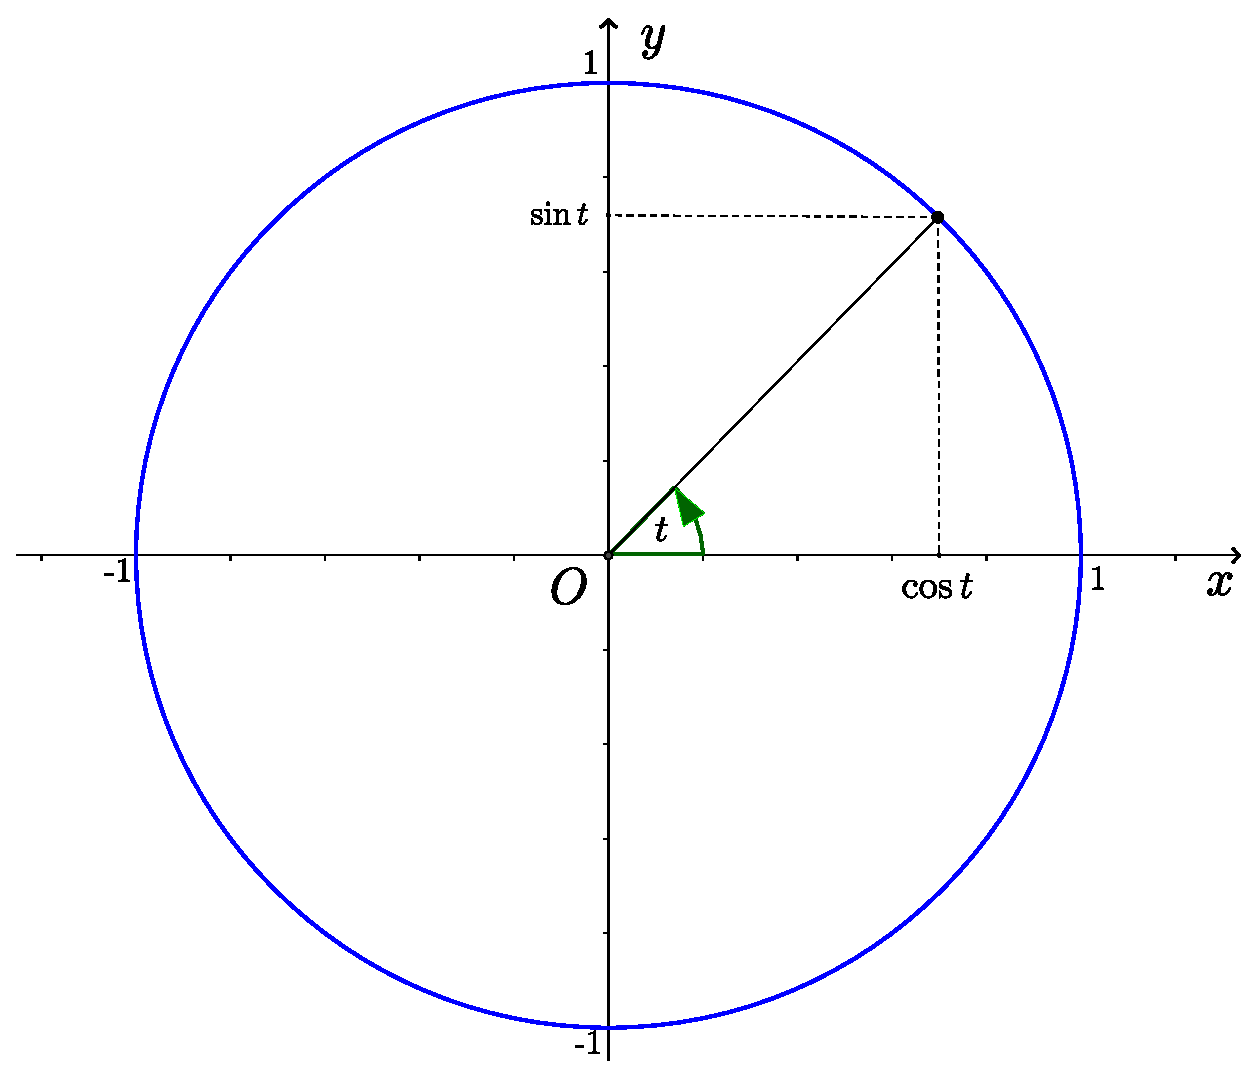
\includegraphics[width=0.5\textwidth]{jednotkovakruznice.eps}
	\caption{Jednotková kružnice}
\end{figure}
\noindent Kružnici můžeme tedy popsat takto
$$k(t)=[\cos{t}, \sin{t}]$$
a to je právě parametrický popis kružnice (také parametrické rovnice kružnice), \textit{t} se nazývá
parametr. Parametr \textit{t} je proměnný a jeho hodnoty můžeme vybírat z různých intervalů: \\
\begin{tabular}{ll}
	$t \in \mathbb{R}$             & kružnice je probíhána neustále                                                                                       \\  
	$t \in \langle 0, 2\pi\rangle$ & výchozí bod je $k(0)=[\cos{0}, \sin{0}] = [1, 0]$                                                                      \\ 
	                               & koncový bod je $k\left(2\pi\right)=[\cos{2\pi}, \sin{2\pi}] = [1, 0]$                                                   \\ 
	                               & jeden oběh kružnice                                                                                                    \\ 
	$t \in \langle 0, 4\pi\rangle$ & výchozí bod je $k(0) = [1, 0]$                                                                                         \\ 
	                               & koncový bod je $k\left(4\pi\right) = [1, 0]$                                                                            \\ 
	                               & dva oběhy kružnice                                                                                                     \\ 
	$t \in \langle 0, \pi\rangle$  & výchozí bod je $k(0) = [1, 0]$                                                                                         \\ 
	                               & koncový bod je $k\left(\pi\right)=[-1, 0]$                                                                              \\ 
	                               & popis půlkružnice (horní půlkružnice)                                                                               \\ 
	$t \in \left\langle -\frac{\pi}{2}, \frac{\pi}{2}\right\rangle$
	                               & výchozí bod je $k\left(-\frac{\pi}{2}\right) = \left[\cos{(-\frac{\pi}{2})}, \sin{(-\frac{\pi}{2})}\right]  = [0, -1]$ \\ 
	                               & koncový bod je $k\left(\frac{\pi}{2}\right) = [0, 1]$                                                                   \\ 
	                               & popis půlkružnice (pravá půlkružnice)                                                                               \\ 
	$t \in \left\langle -\frac{3\pi}{4}, \frac{\pi}{3}\right\rangle$
	                               & výchozí bod je $k\left(-\frac{3\pi}{4}\right)  = \left[-\frac{\sqrt{2}}{2}, -\frac{\sqrt{2}}{2} \right]$               \\ 
	                               & koncový bod je $k\left(\frac{\pi}{3}\right)  = \left[\frac{1}{2}, \frac{\sqrt{3}}{2} \right]$                           \\ 
	                               & popis části kružnice                                                                                                  \\ 
\end{tabular}\\
\begin{figure}
	\centering
	\begin{subfigure}[b]{0.3\textwidth}
		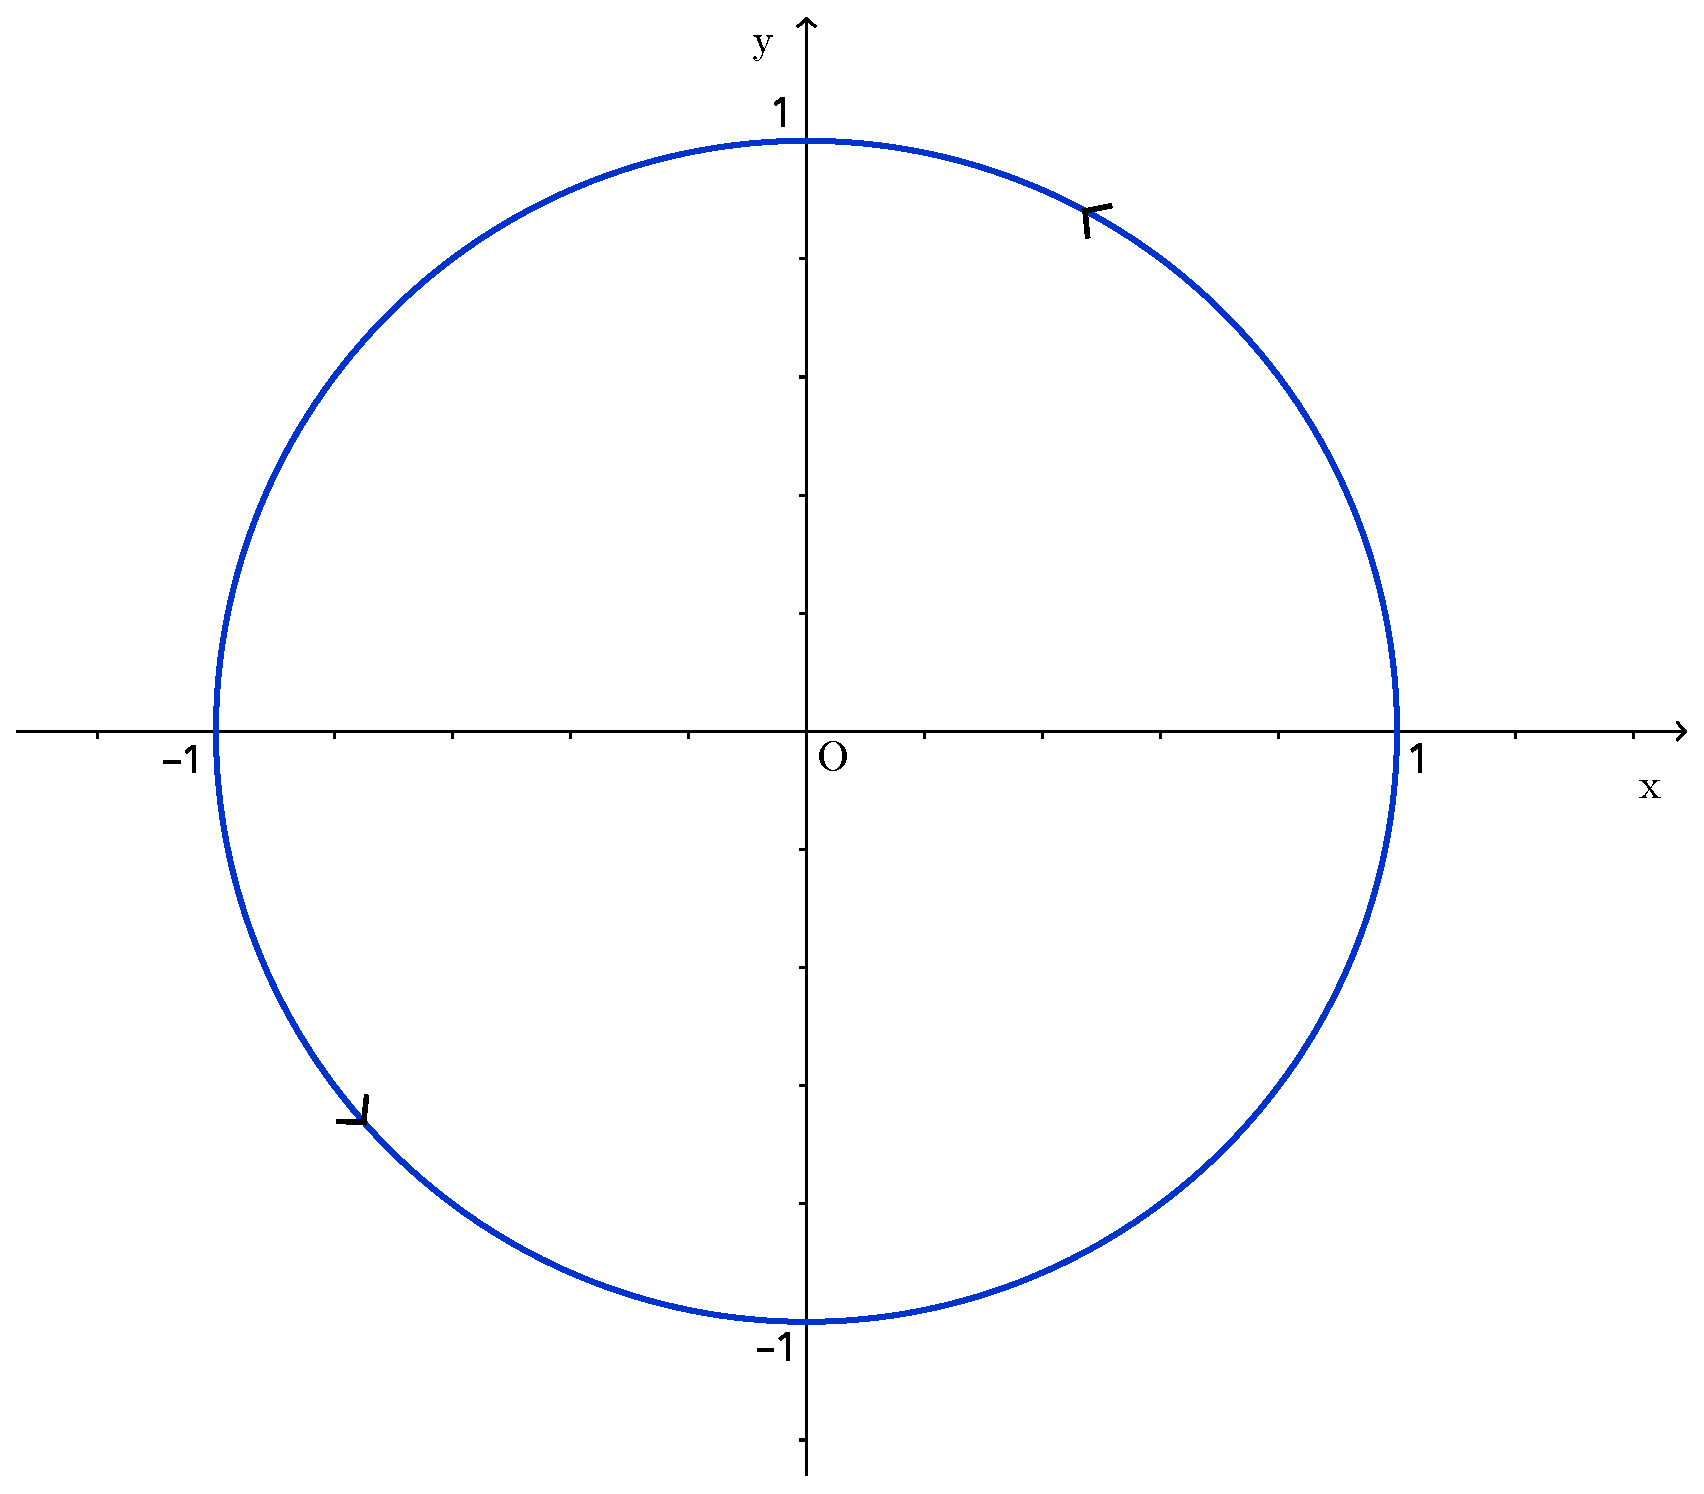
\includegraphics[width=\textwidth]{kruznice-teorie1.eps}
		\caption{$t \in \mathbb{R}$}
	\end{subfigure}%
	\quad
	\begin{subfigure}[b]{0.3\textwidth}
		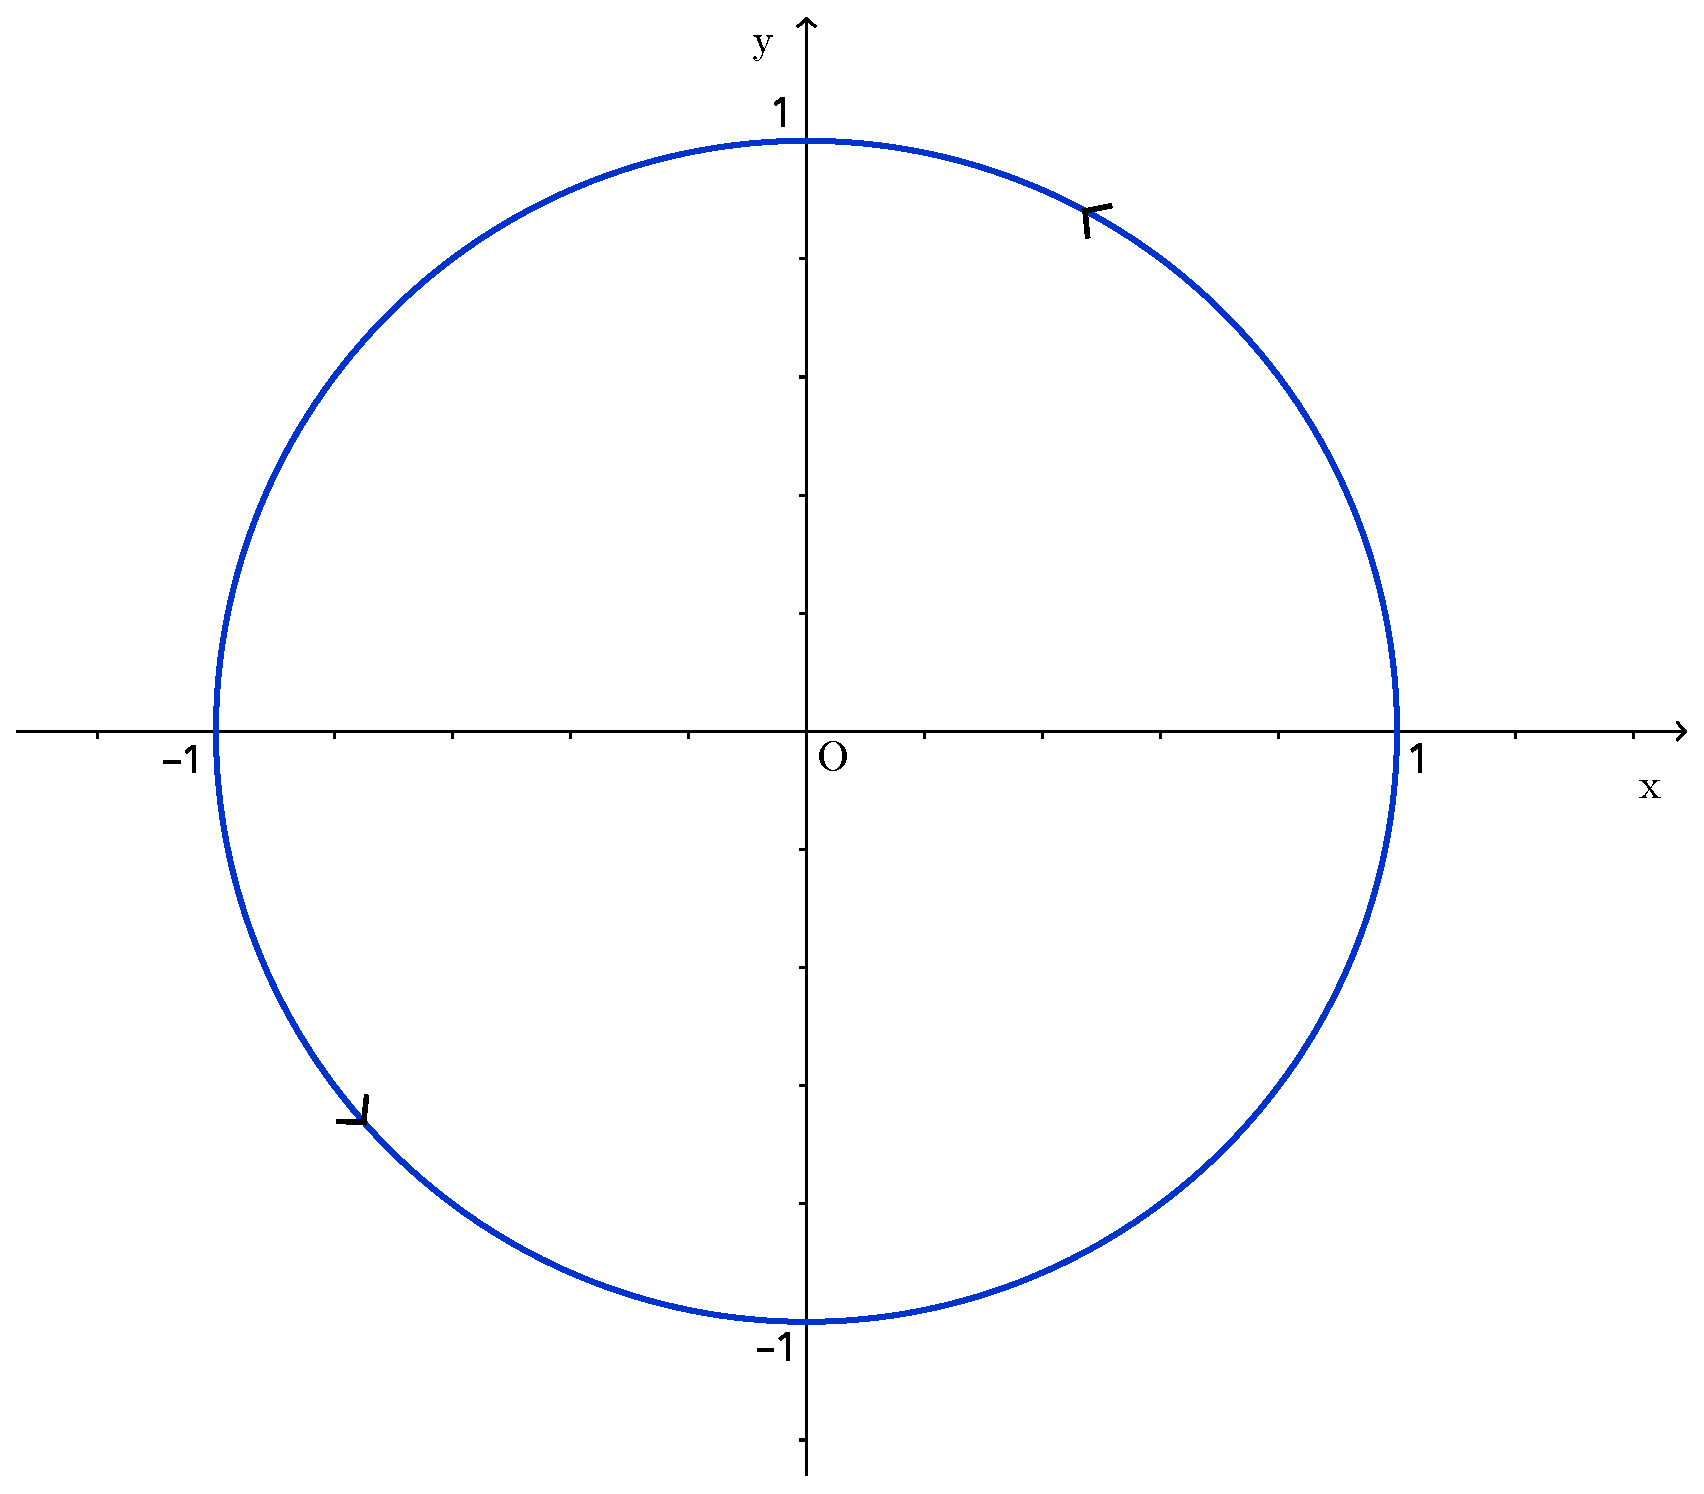
\includegraphics[width=\textwidth]{kruznice-teorie1.eps}
		\caption{$t \in \langle 0, 2\pi\rangle$}
	\end{subfigure}%
	\quad
	\begin{subfigure}[b]{0.3\textwidth}
		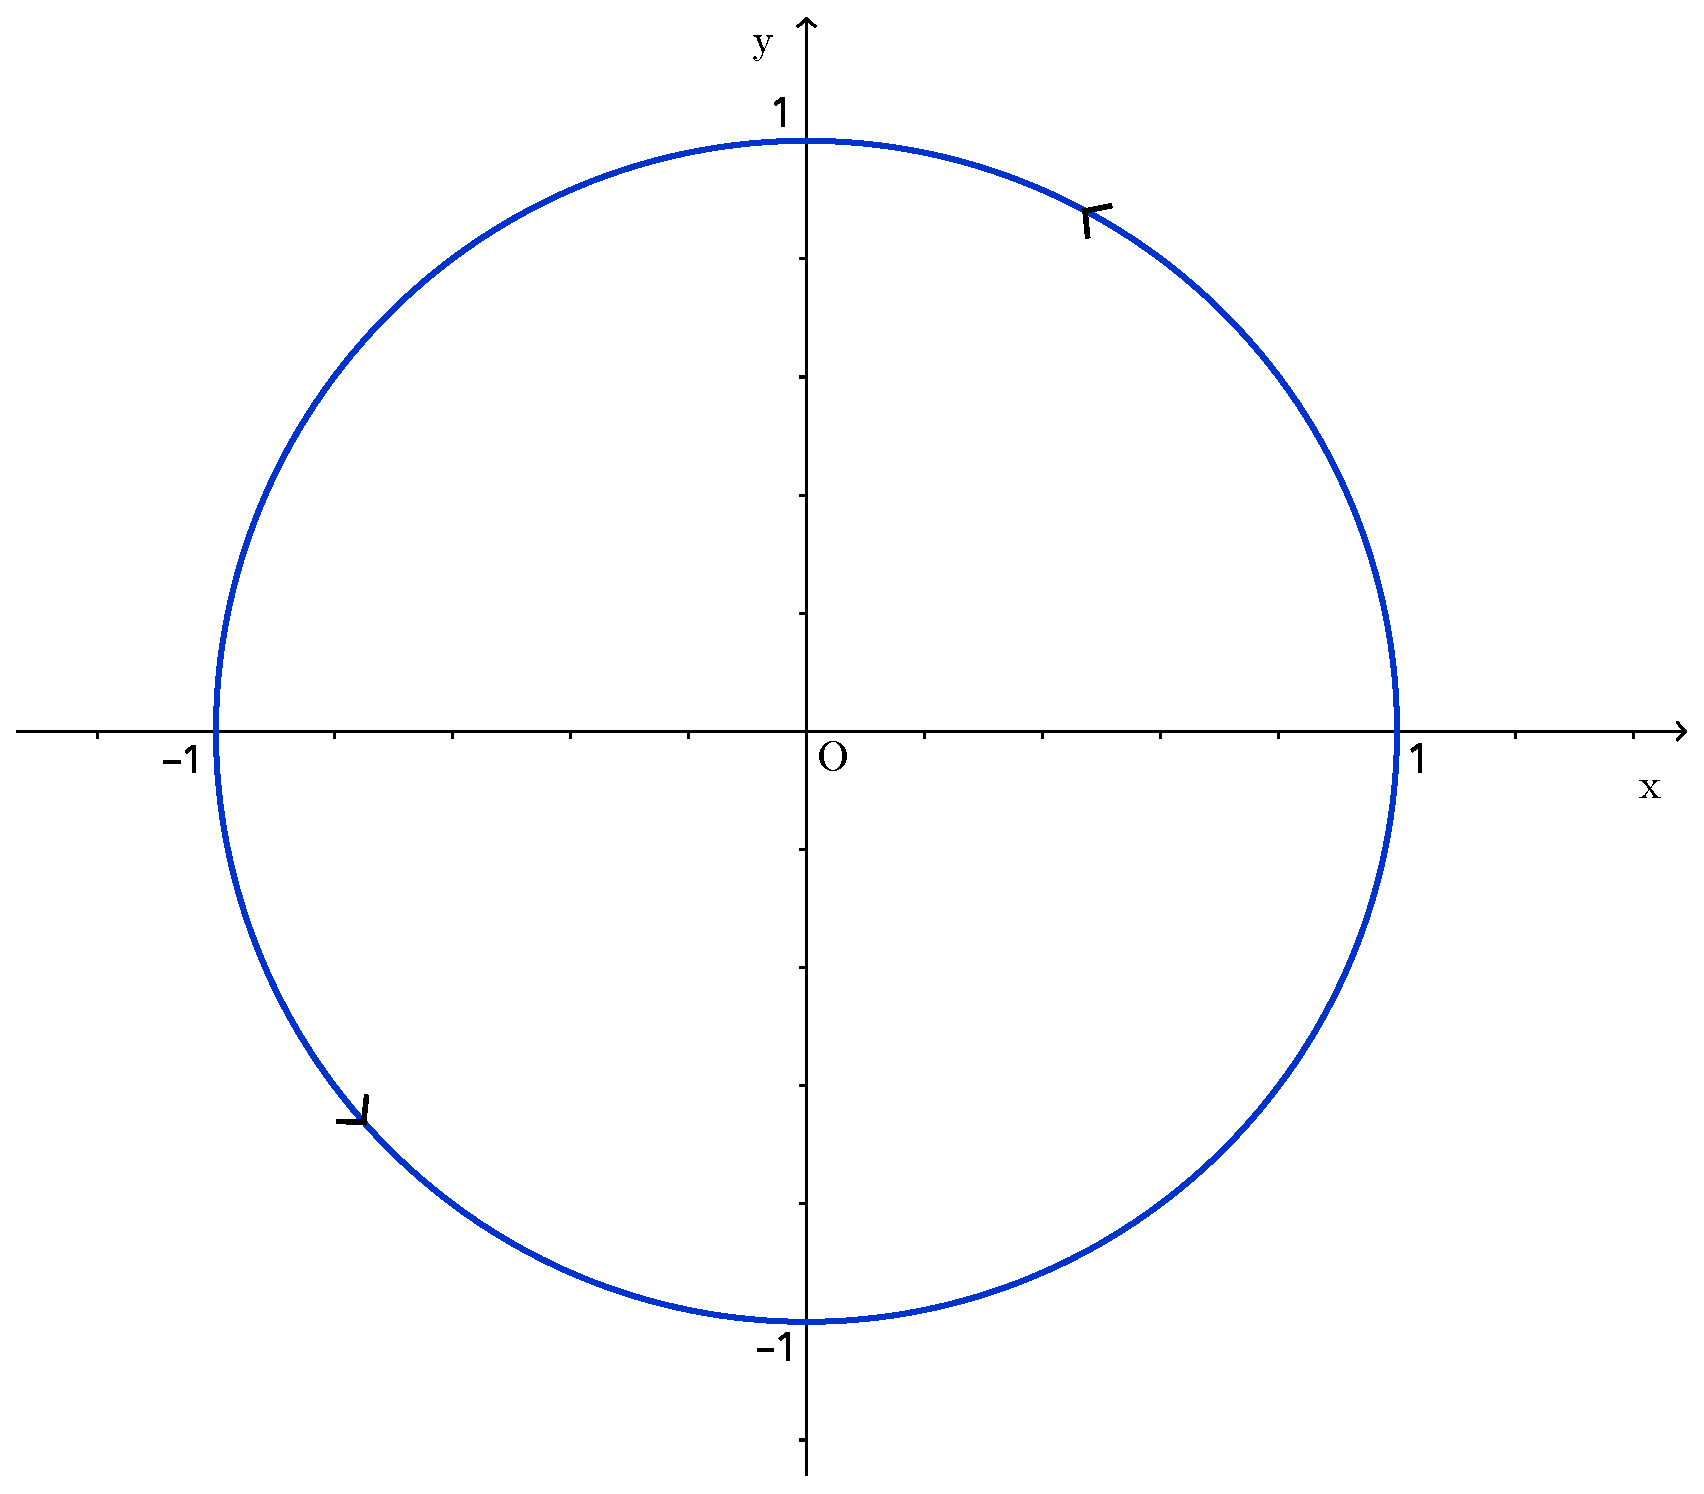
\includegraphics[width=\textwidth]{kruznice-teorie1.eps}
		\caption{$t \in \langle 0, 4\pi\rangle$}
	\end{subfigure}%
	\\
	\begin{subfigure}[b]{0.33\textwidth}
		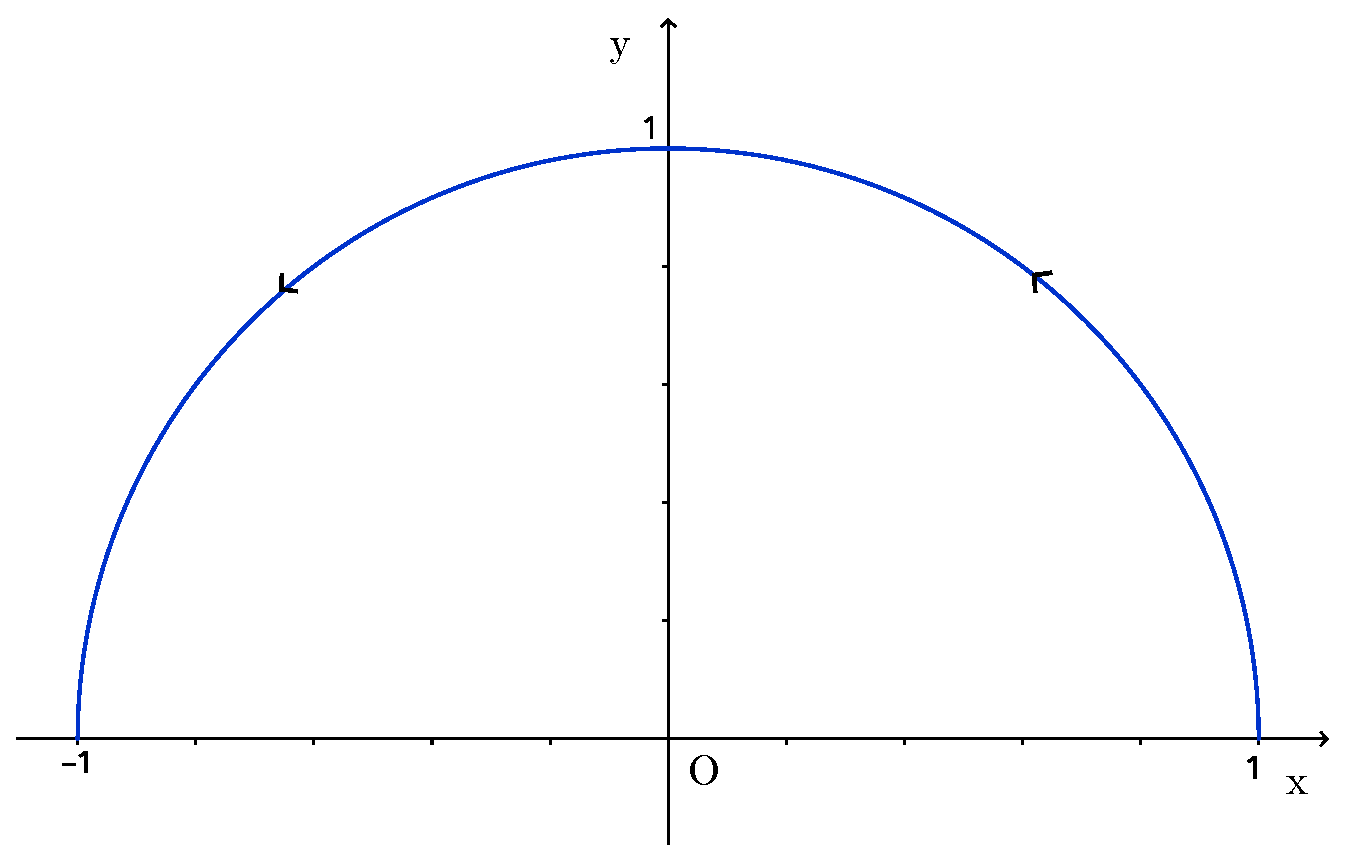
\includegraphics[width=\textwidth]{kruznice-teorie2.eps}
		\caption{$t \in \langle 0, \pi\rangle$}
	\end{subfigure}%
	\begin{subfigure}[b]{0.33\textwidth}
		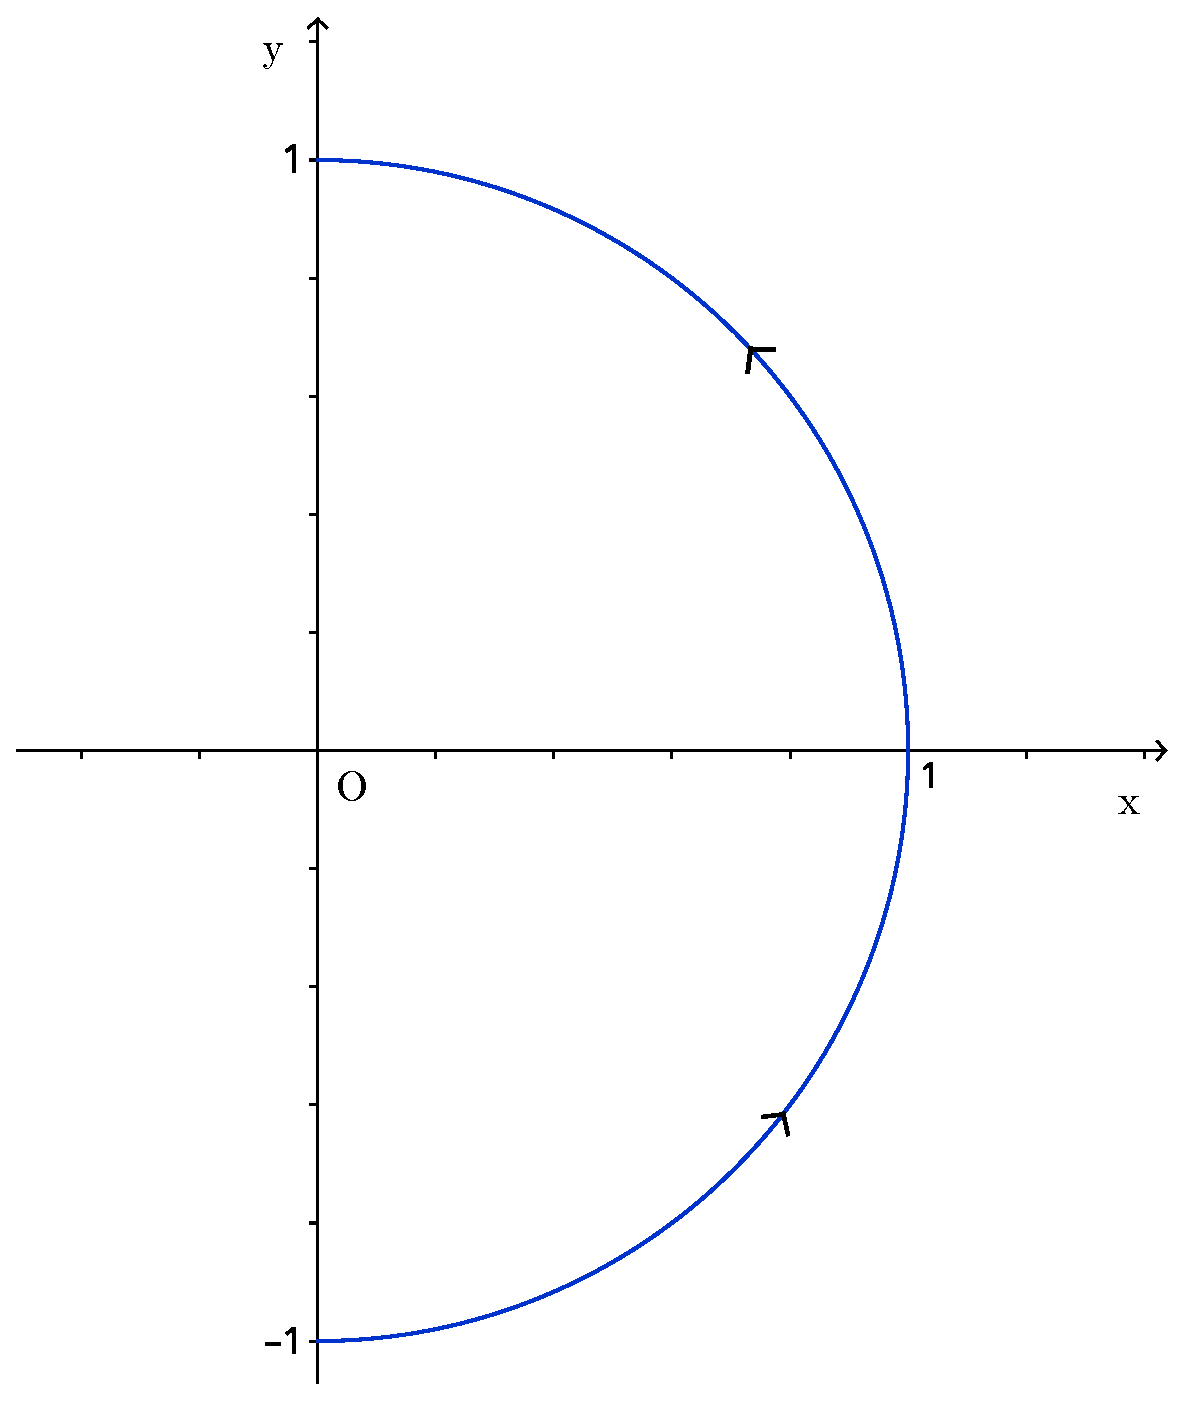
\includegraphics[width=\textwidth]{kruznice-teorie3.eps}
		\caption{$t \in \left\langle -\frac{\pi}{2}, \frac{\pi}{2}\right\rangle$}
	\end{subfigure}%
	\begin{subfigure}[b]{0.33\textwidth}
		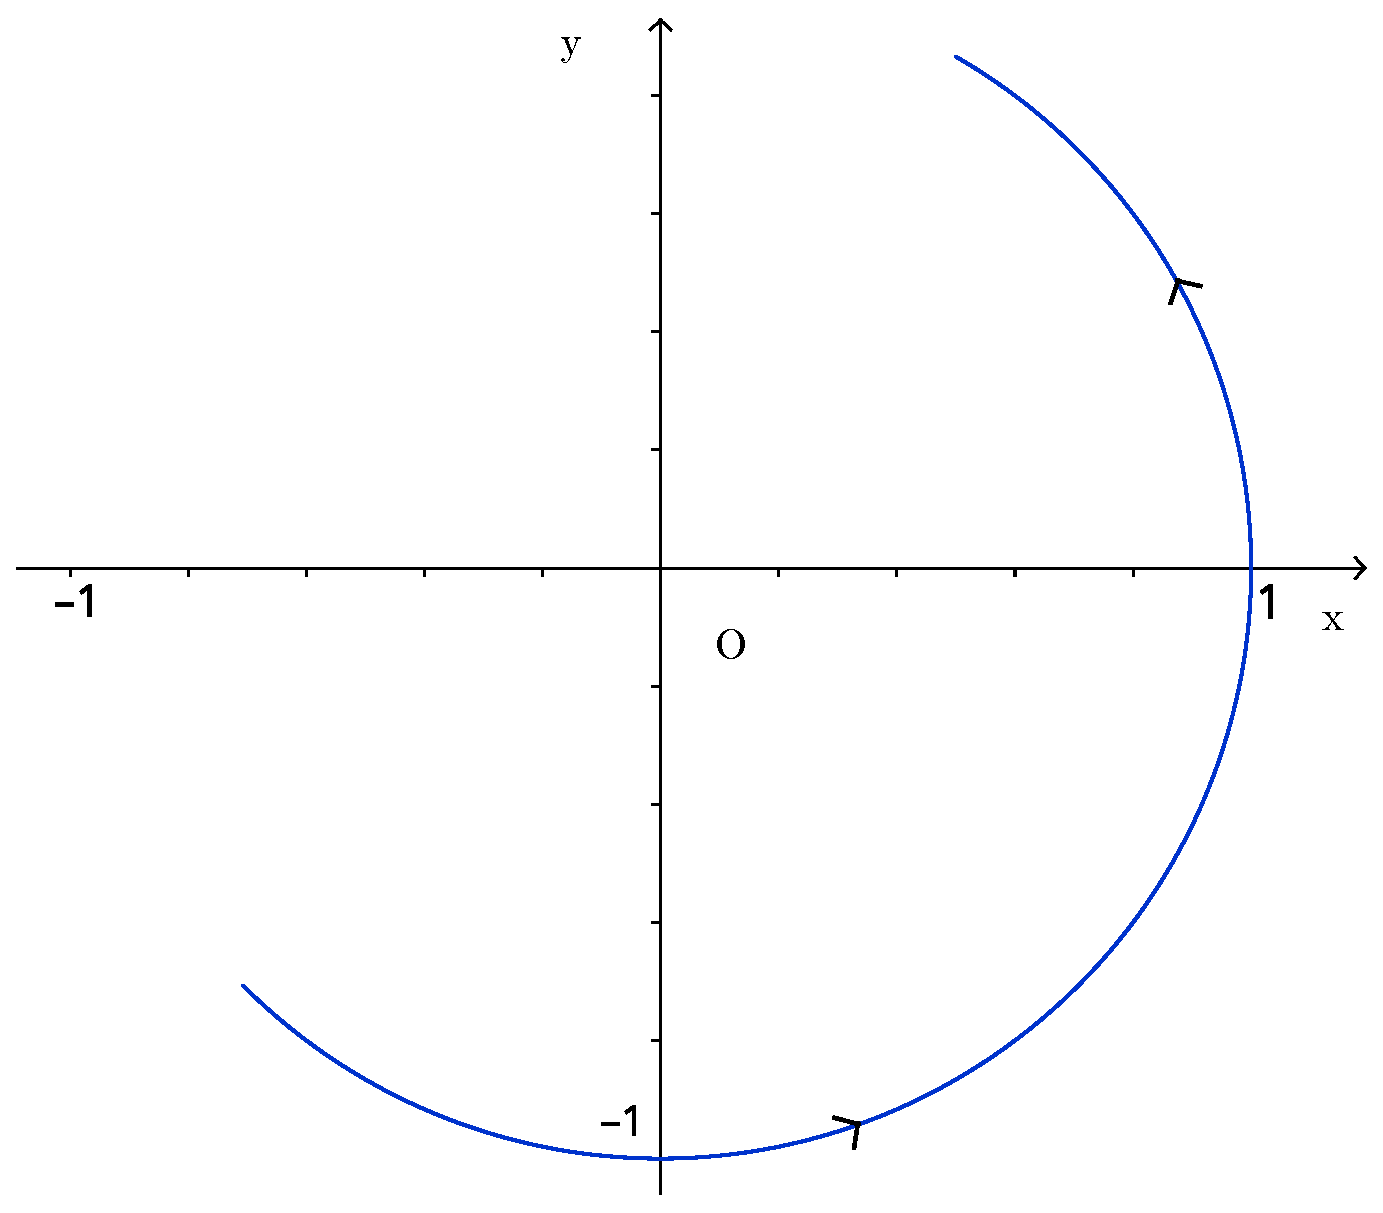
\includegraphics[width=\textwidth]{kruznice-teorie4.eps}
		\caption{$t \in \left\langle -\frac{3\pi}{4}, \frac{\pi}{3}\right\rangle$}
	\end{subfigure}%
	\caption{Kružnice \textit{k} pro různé intervaly parametru \textit{t}}
\end{figure}
\\
\noindent{}Při parametrickém vyjádření $k(t) = [\cos{t}, \sin{t}]$ je kružnice, či její část, probíhána vždy v kladném směru
(tj. proti směru hodinových ručiček). \\
Jak parametrický popis upravit, aby byla kružnice nebo její část probíhána v záporném směru? Zkusíme zaměnit parametr \textit{t} hodnotou $-t$:
$$k(t)=[\cos{(-t)}, \sin{(-t)}] = [\cos{t}, -\sin{t}]$$
(využíváme, že $\cos$ je sudá funkce a $\sin$ je lichá funkce). \\[5pt]
Uvažujme pro parametr \textit{t} interval $ \langle 0, 2\pi\rangle$. \\
Snadno vypočítáme $k(0)=[1,0]$, $k\left(\frac{\pi}{2}\right)=[0,-1]$, 
$k(\pi)=[-1,0]$ a $k(2\pi)=[1,0]$. Výchozí i koncový bod je $[1, 0]$
a kružnice je probíhána v záporném směru (tj. ve směru hodinových ručiček). \\
Můžeme vyzkoušet i další kombinace. Pro jeden oběh kružnice je výhodné použít vždy interval $\langle0, 2\pi \rangle$. \\
\begin{tabular}{ll}
	$k(t)=[-\cos{t}, \sin{t}]$  & výchozí bod je $k(0)=[-1, 0]$                                           \\ 
	                            & pro určení směru použijeme bod $k\left(\frac{\pi}{2}\right) = [0, 1]$ \\ 
	                            & tj. kružnice je probíhána v záporném směru                          \\ 
	$k(t)=[-\cos{t}, -\sin{t}]$ & výchozí bod je $k(0) = [-1, 0]$                                         \\ 
	                            & $k\left(\frac{\pi}{2}\right) = [0, -1]$                                   \\ 
	                            & tj. kružnice je probíhána v kladném směru                            \\ 
\end{tabular}  \\[5pt]
Ještě můžeme zaměnit souřadnice (stále $t \in \langle0, 2\pi\rangle$): \\
\begin{tabular}{llll}
	$k(t)=[\sin{t}, \cos{t}]$   & $k(0)=[0, 1]$  & $k\left(\frac{\pi}{2}\right) = [1,0]$  & záporný směr \\ 
	$k(t)=[\sin{t}, -\cos{t}]$  & $k(0)=[0, -1]$ & $k\left(\frac{\pi}{2}\right) = [1,0]$  & kladný směr   \\ 
	$k(t)=[-\sin{t}, \cos{t}]$  & $k(0)=[0, 1]$  & $k\left(\frac{\pi}{2}\right) = [-1,0]$ & kladný směr   \\ 
	$k(t)=[-\sin{t}, -\cos{t}]$ & $k(0)=[0, -1]$ & $k\left(\frac{\pi}{2}\right) = [-1,0]$ & záporný směr \\ 
\end{tabular}  \\[5pt]
Pro kružnici, která má střed $[0, 0]$ a její poloměr \textit{r} není roven 1, lze využít podobné popisy
$k(t) = [r\cdot\cos{t}, r\cdot\sin{t}]$, $k(t) = [r\cdot\cos{t}, -r\cdot\sin{t}]$ atd. \\[10pt]
	Ve všech předchozích popisech jednotkové kružnice, kde $t \in \langle0, 2\pi\rangle$, je výchozí bod
	na jedné ze souřadnicových os \textit{x} a \textit{y}. Jak popsat kružnici, aby výchozí bod mohl být
	vybrán obecněji? Jistě bychom mohli změnit interval pro parametr \textit{t}, $t \in \langle\alpha, \beta\rangle$,
	ale určení úhlu $\alpha$ nemusí být vždy jednoduché. Chceme vždy použít pro jeden oběh interval $\langle0, 2\pi\rangle$.
	Vyberme bod $\left[\frac{1}{2}, \frac{\sqrt{3}}{2}\right]$ na jednotkové kružnici. Chceme, aby tento bod byl výchozí
	a kružnice byla probíhána v kladném směru. \\
	Požadujeme $k(0)=\left[\frac{1}{2}, \frac{\sqrt{3}}{2}\right]$ a
	$k\left(\frac{\pi}{2}\right)=\left[-\frac{\sqrt{3}}{2}, \frac{1}{2}\right]$.
	\begin{figure}[H]
		\centering
		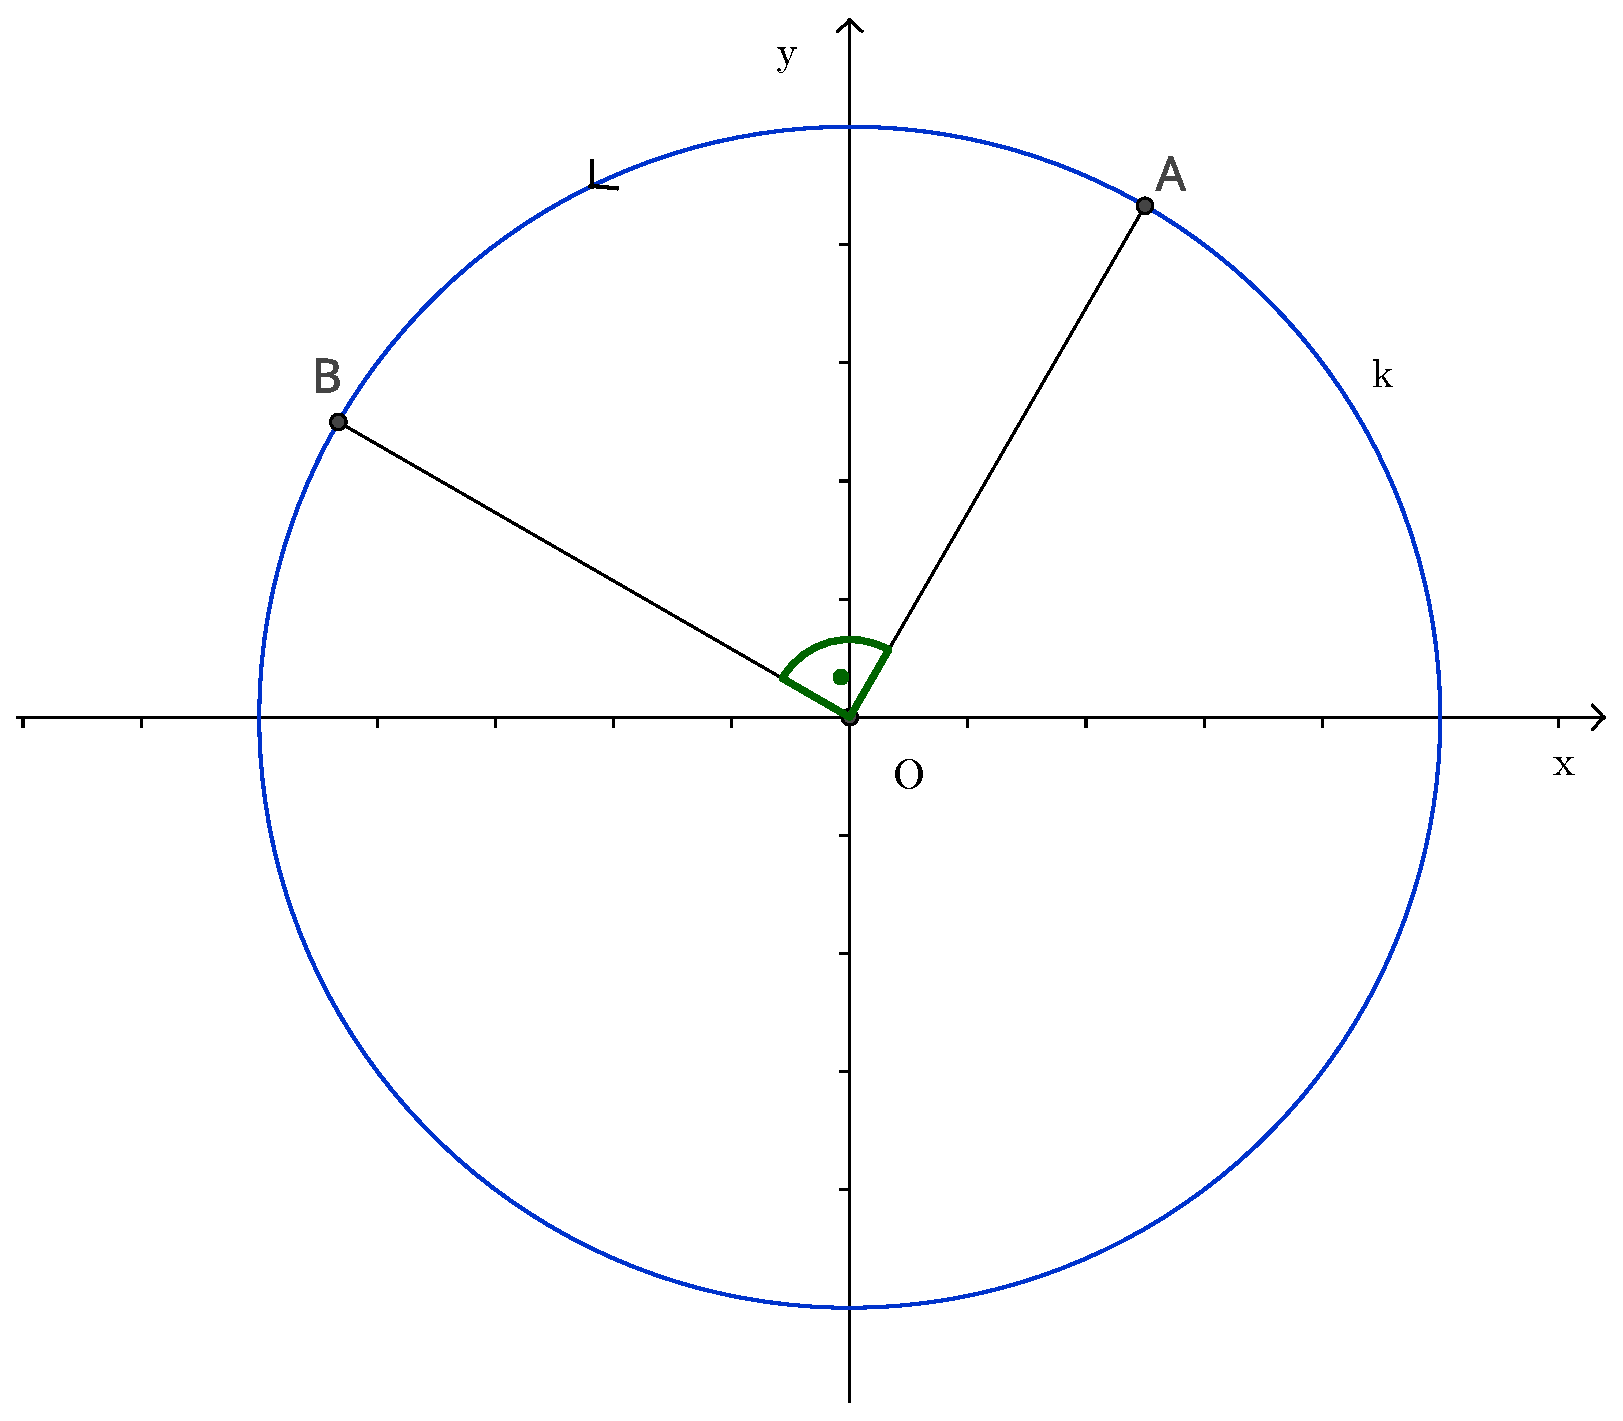
\includegraphics[width=0.45\textwidth]{kruznice-teorie5.eps}
		\caption{Kružnice probíhána z obecného bodu}					
	\end{figure}
	V první i druhé souřadnici parametrického popisu se musí objevit funkce $\cos$ i $\sin$:
	$$ k(t) = \left[\frac{1}{2}\cos{t}-\frac{\sqrt{3}}{2}\sin{t}, \frac{\sqrt{3}}{2}\cos{t}+\frac{1}{2}\sin{t}\right], t \in \langle0, 2\pi\rangle. $$
	Pro oběh kružnice v záporném směru stačí změnit znaménka u funkce $\sin$, jak jsme mohli vypozorovat v předchozím popisu. \\
	Pro kružnici o středu $S=[0, 0]$ a pro výchozí bod $P=[p, q]$ můžeme psát
	$$k(t) = [p\cos{t}-q\sin{t}, q\cos{t} + p\sin{t}], t \in \langle0, 2\pi\rangle \text{, kladný směr},$$
	$$k(t) = [p\cos{t}+q\sin{t}, q\cos{t} - p\sin{t}], t \in \langle0, 2\pi\rangle \text{, záporný směr}.$$
	Lze také použít zápis s využitím vektorů
	$$k(t) = [0, 0] + (p, q)\cos{t}+(-q, p)\sin{t}$$ nebo
	$$k(t) = [0, 0] + (p, q)\cos{t}+(q, -p)\sin{t},$$
	$[0, 0]$ je střed \textit{S}, vektor $(p, q) = P - S$, vektor $(-q, p)$ nebo $(q, -p)$ je kolmý k vektoru $P-S$. \\	
	\noindent Nyní již snadno získáme parametrický popis libovolné kružnice o středu $S=[m, n]$, jejíž výchozí bod je
	bod $P=[p, q]$:
	\begin{figure}[H]
		\centering
		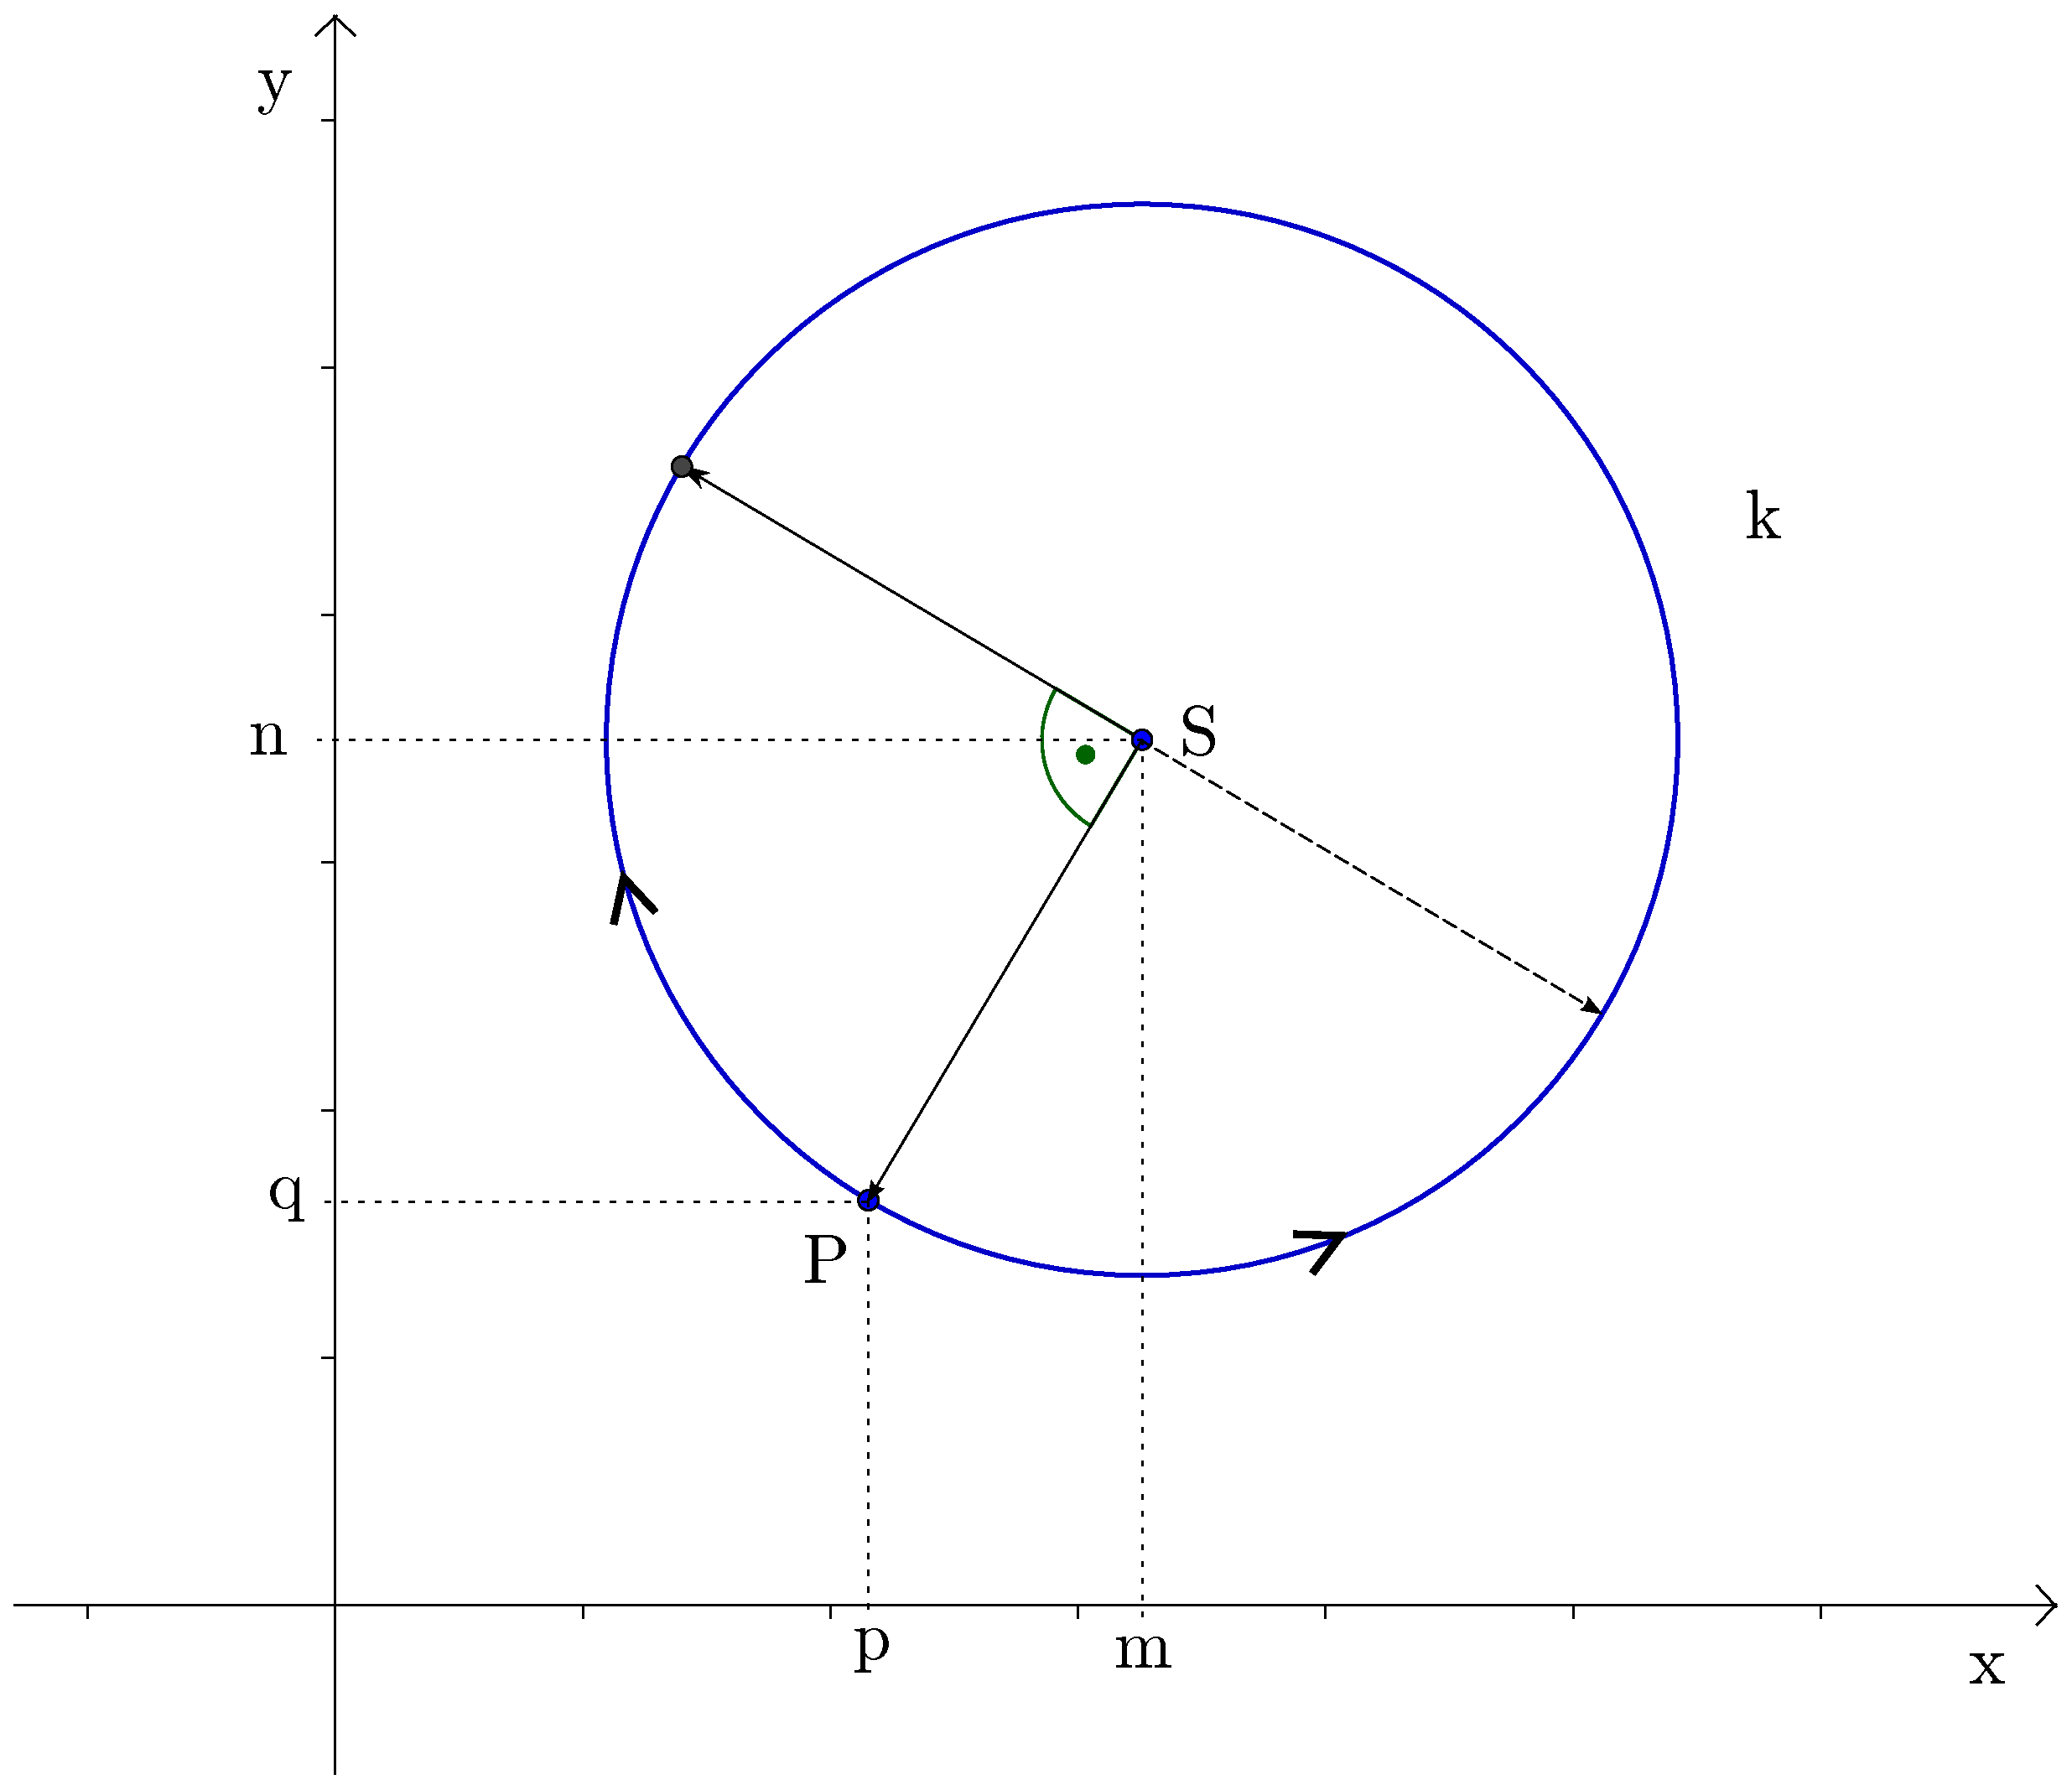
\includegraphics[width=0.5\textwidth]{kruznice-teorie7.eps}
		\caption{Libovolná kružnice probíhána z obecného bodu}					
	\end{figure}	
	$$P-S = (p-m, q-n)$$
	a vektor kolmý je
	$$(-(q-n), p-m), \text{pro kladný směr}$$
	nebo
	$$(q-n, -(p-m)), \text{pro záporný směr}.$$
	Tedy
	$$k(t)=[m, n] + (p-m, q-n)\cos{t} + (-(q-n), p-m)\sin{t}, $$
	tj.:
	$$k(t)=[m + (p-m)\cos{t} - (q-n)\sin{t}, n + (q-n)\cos{t}+(p-m)\sin{t}], t \in \langle0, 2\pi\rangle.$$
	kružnice probíhána (1 oběh) od bodu \textit{P} v kladném směru. \\
	Pro změnu směru stačí změnit znaménko u funkce $\sin$. \\[5pt]
	Tento popis nevyžaduje znalost poloměru kružnice, poloměr si lze ovšem vždy spočítat, je to vzdálenost
	bodů \textit{P}, \textit{S}:
	$$r=\sqrt{(p-m)^2+(q-n)^2}.$$
	Je vidět, že parametrický popis má oproti obecné rovnici navíc důležitou informaci. Parametr \textit{t} si
	můžeme představit jako čas a z parametrického popisu lze vyčíst, jak je křivka probíhána v čase.
	\clearpage
	\subsection*{Příklad}
	Napište parametrické vyjádření kružnice zadané obecnou rovnicí
	$$x^2+y^2-6x-8y=0.$$
	Ověřte, zda kružnice prochází počátkem soustavy souřadné. Pokud ano, napište parametrické
	vyjádření kružnice (jeden oběh), výchozí bod nechť je počátek $[0, 0]$ a kružnice je probíhána
	v záporném směru. \\[10pt]
	\textbf{Řešení:}
	\begin{enumerate}
		\item Obecnou rovnici upravíme na středový tvar
		      $$(x-3)^2+(y-4)^2=25, \text{popř. } \frac{(x-3)^2}{25} + \frac{(y-4)^2}{25}=1.$$
		      Bod $S=[3, 4]$ je střed, poloměr $r=5$. Pokud nám nezáleží, jakým způsobem je kružnice
		      probíhána, můžeme využít vzorec
		      $$\cos^2{t}+\sin^2{t}=1.$$
		      Dáme do rovnosti
		      $$\frac{x-3}{5} = \cos{t}$$
		      a
		      $$\frac{y-4}{5}=\sin{t}$$
		      (nebo $\frac{x-3}{5} = \sin{t}$ a $\frac{y-4}{5}=\cos{t}$). \\
		      Vyjádříme \textit{x} a \textit{y}:
		      $$x=3+5\cos{t},$$
		      $$y=4+5\sin{t}.$$
		      Parametrický popis kružnice je
		      $$k(t) = [3+5\cos{t}, 4+5\sin{t}], t \in \langle0,2\pi\rangle. $$
		      Dosazením $t=0$ a $t=\frac{\pi}{2}$
		      $$k(0) = [8, 4], k\left(\frac{\pi}{2}\right) = [3, 9]$$
		      zjistíme, že výchozí bod je $[8, 4]$ a kružnice je probíhána v kladném směru.
		\item Bod $[0, 0]$ je bodem kružnice (dosadíme do zadané rovnice $x=0$ a $y=0$). \\
		      Nyní můžeme použít vzorec
		      $$k(t)=[m + (p-m)\cos{t} + (q-n)\sin{t}, n + (q-n)\cos{t}-(p-m)\sin{t}], t \in \langle0, 2\pi\rangle$$
		      kde $[m, n] = [3, 4], [p, q] = [0, 0]$. \\[5pt]
		      	Nebo můžeme vyjádřit vektor $O-S=[0, 0] - [3, 4] = (-3, -4)$ a vektor kolmý $(-4, 3)$: \\
		      	$$k(t) = [3, 4] + (-3, -4)\cos{t}+(-4, 3)\sin{t}, t \in \langle0, 2\pi\rangle.$$
		      	$$k(t) = [3-3\cos{t}-4\sin{t}, 4-4\cos{t}+3\sin{t}], t \in \langle0, 2\pi\rangle.$$
		      \end{enumerate}
		      \begin{figure}[H]
		      	\centering
		      	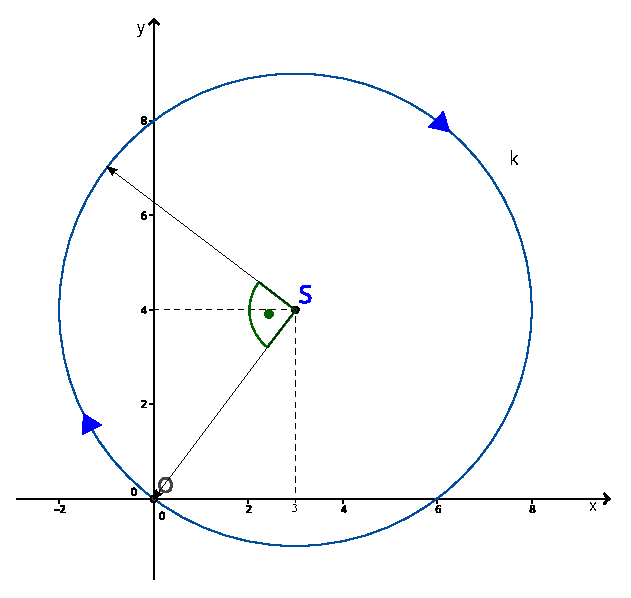
\includegraphics[height = 275pt]{kruznice4.eps}
		      	\caption{Kružnice probíhána v záporném směru  pro $t \in \langle0, 2\pi\rangle$}
		      						
		      \end{figure}
		      \clearpage
		      \section{Parabola}
		      Uvažujme známou parabolu $y=x^2$.\\
		      Tato rovnice je ve vrcholovém tvaru a vrchol paraboly je bod $[0,0]$, osa paraboly je osa \textit{y}. \\
		      Parametr \textit{p} je $p=\frac{1}{2}$ ($x^2=2py$, $2p=1$).
		      Parametr je vzdálenost ohniska \textit{F} od řídící přímky \textit{d}. Ohnisko má souřadnice $F=\left[0, \frac{1}{4}\right]$, řídící přímka má obecnou rovnici $d: y=-\frac{1}{4}$.
		      \begin{figure}[H]
		      	\centering
		      	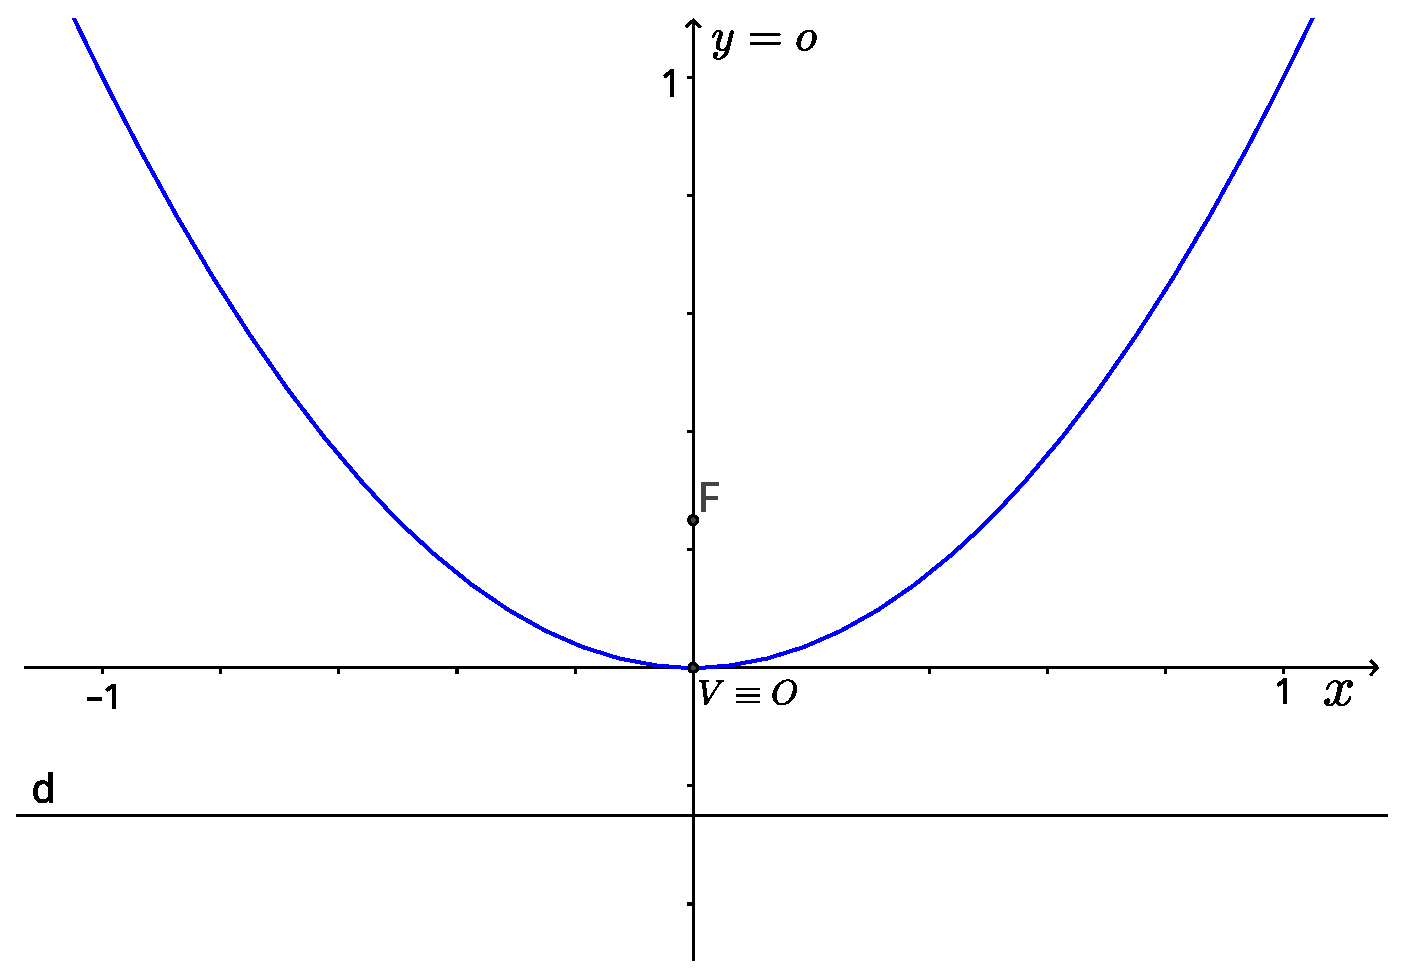
\includegraphics[width=0.5\textwidth]{parabola-teorie1.eps}
		      	\caption{Parabola $y=x^2$}
		      \end{figure}
		      \noindent Souřadnice libovolného bodu jsou $[x, x^2]$. \\
		      Parametrický popis této paraboly je např.:
		      $$k(t) = [t, t^2].$$
		      Aby byla popsána celá parabola, je potřeba pro parametr \textit{t} brát interval $(-\infty, \infty)$, $k(0)=[0,0]$. \\
		      Při kreslení paraboly s využitím grafického programu musíme interval omezit z obou stran, např. $t \in \langle-10, 10\rangle$.
		      \clearpage
		      Parametrických popisů zadané paraboly je stejně jako u kružnice nekonečné mnoho a liší se tím, jak je parabola probíhána.
		      $$k(t)=[t, t^2], t \in \langle-3,3\rangle$$
		      \begin{figure}[H]
		      	\centering
		      	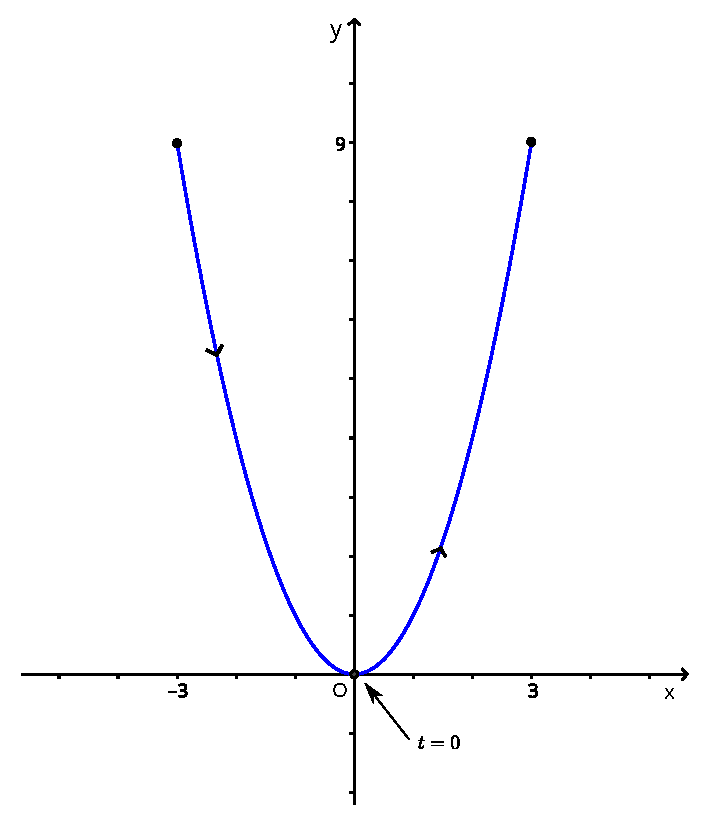
\includegraphics[width=0.4\textwidth]{parabola-teorie2.eps}
		      	\caption{Parabola \textit{k} pro $t \in \langle-3,3\rangle$}
		      \end{figure}
		      $$k(t)=[-t, t^2], t \in \langle-3,3\rangle$$
		      \begin{figure}[H]
		      	\centering
		      	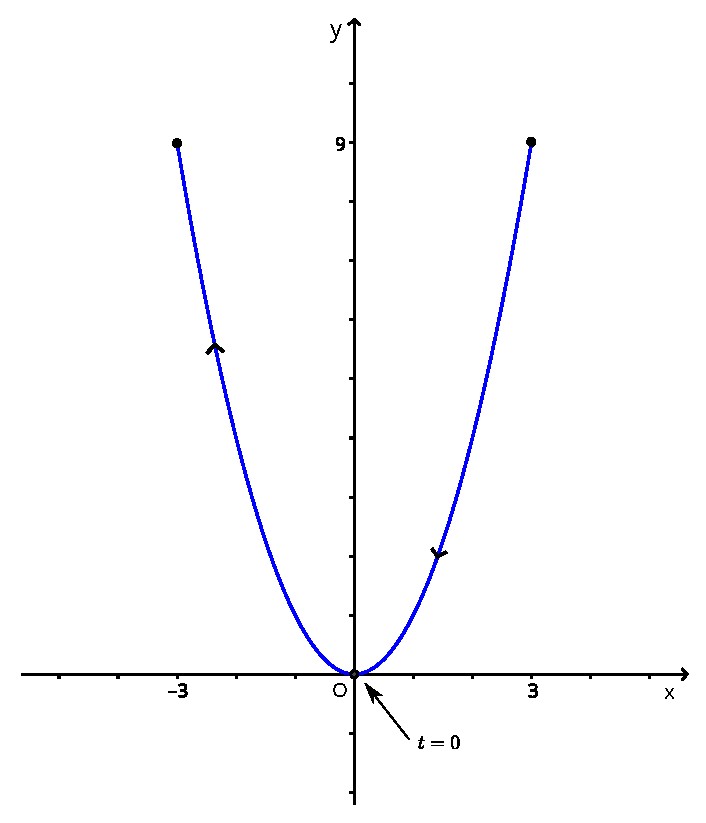
\includegraphics[width=0.4\textwidth]{parabola-teorie3.eps}
		      	\caption{Parabola \textit{k} pro $t \in \langle-3,3\rangle$}
		      \end{figure}
		      $$k(t)=[t+1, (t+1)^2], t \in \langle-3,3\rangle$$
		      \begin{figure}[H]
		      	\centering
		      	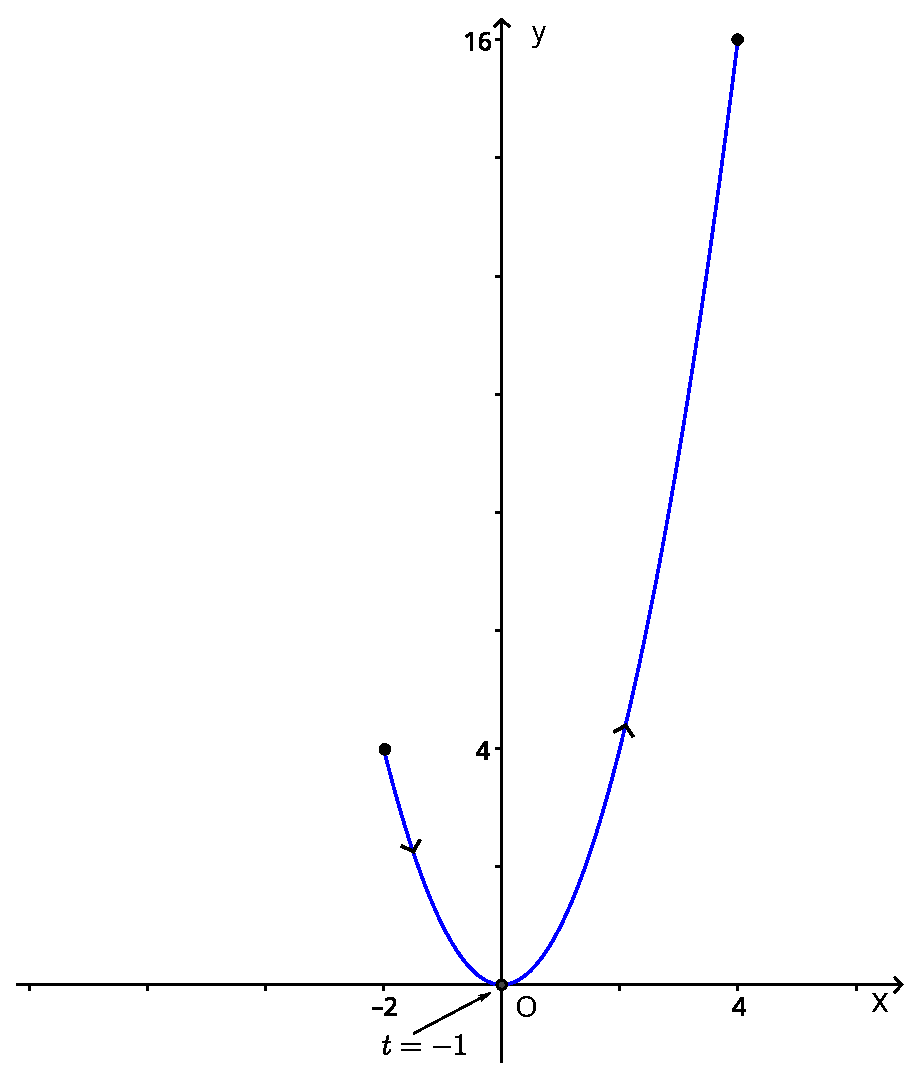
\includegraphics[width=0.4\textwidth]{parabola-teorie4.eps}
		      	\caption{Parabola \textit{k} pro $t \in \langle-3,3\rangle$}
		      \end{figure}
		      $$k(t)=[1-t, (1-t)^2], t \in \langle-3,3\rangle$$
		      \begin{figure}[H]
		      	\centering
		      	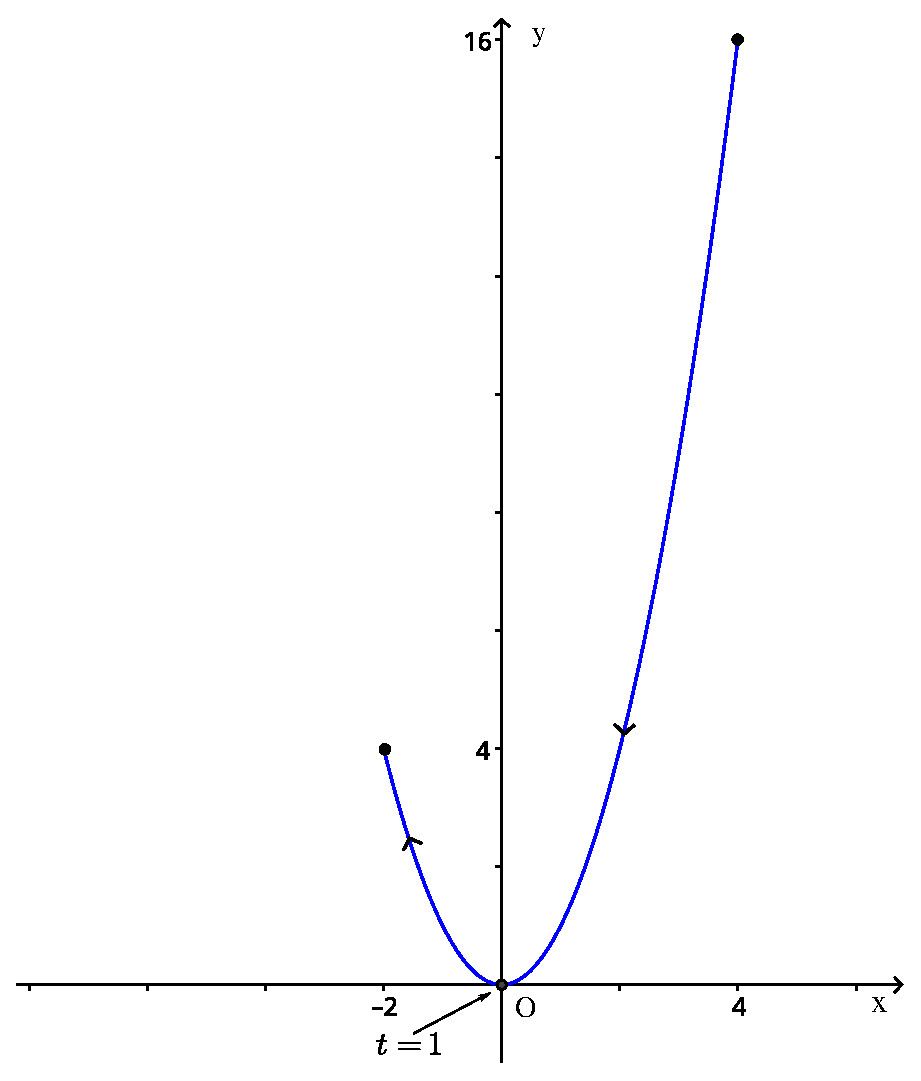
\includegraphics[width=0.4\textwidth]{parabola-teorie5.eps}
		      	\caption{Parabola \textit{k} pro $t \in \langle-3,3\rangle$}
		      \end{figure}
		      \clearpage
		      Podobně můžeme postupovat pro další paraboly \\
		      \begin{center}
		      	\begin{tabular}{ccc}
		      		$x^2=-2py$ & $x=t$, $t^2=-2py$ & $k(t)=\left[t, -\frac{t^2}{2p}\right], t \in \mathbb{R}$, \\ 
		      		$y^2=2px$  & $y=t$, $t^2=2px$  & $k(t)=\left[\frac{t^2}{2p}, t\right], t \in \mathbb{R}$,  \\ 
		      		$y^2=-2px$ & $y=t$, $t^2=-2px$ & $k(t)=\left[-\frac{t^2}{2p}, t\right], t \in \mathbb{R}$. 
		      	\end{tabular} 
		      \end{center}
		      V případě parabol s vrcholem $V=[m, n]$ volíme často parametrizaci tak, aby $k(0)=V$. Volbou intervalu pro parametr \textit{t} snadno vybereme požadovanou část paraboly.
		      Např. 
		      \begin{align*}
		      	(x-m)^2 = 2p(y-n),                                            \\
		      	t       = x-m,\quad x = t+m,                                  \\
		      	t^2     = 2p(y-n), \quad y = \frac{t^2}{2p}+n,                \\
		      	k(t)    = \left[t+m, \frac{t^2}{2p}+n\right], t\in\mathbb{R}, 
		      \end{align*}
		      \begin{align*}
		      	(y-n)^2 = -2p(x-m),                                            \\
		      	t       = y-n,\quad y = t+n,                                   \\
		      	t^2     = -2p(x-m),\quad  x = -\frac{t^2}{2p}+m,               \\
		      	k(t)    = \left[-\frac{t^2}{2p}+m, t+n\right], t\in\mathbb{R}. 
		      \end{align*}
		      \clearpage
		      \subsection*{Příklad 1}
		      Napište parametrické vyjádření paraboly zadané obecnou rovnicí
		      $$x^2-6x-10y+49=0.$$
		      Napište parametrické vyjádření části paraboly mezi jejími body \textit{P} a \textit{Q}, jejichž \textit{y}-ové
		      souřadnice jsou rovny $\frac{13}{2}$. \\[5pt]
		      \textbf{Řešení:}
		      \noindent\begin{enumerate}
		      \item Obecnou rovnici upravíme na vrcholový tvar
		      $$(x-3)^2=10(y-4).$$
		      Bod $V=[3,4]$ je vrchol, parametr $p=5$, ohnisko $F=\left[3,\frac{13}{2}\right]$,  řídící přímka $d: y=\frac{3}{2}$.
		      Volíme $t=x-3$, pak $t^2=10(y-4)$. Vypočítáme $x=t+3$, $y=\frac{t^2}{10}+4$.\\
		      Parametrické vyjádření paraboly je
		      $$k(t)=\left[t+3,\frac{t^2}{10}+4\right], t \in \mathbb{R}.$$
		      \vfill
		      \begin{figure}[H]
		      	\centering
		      	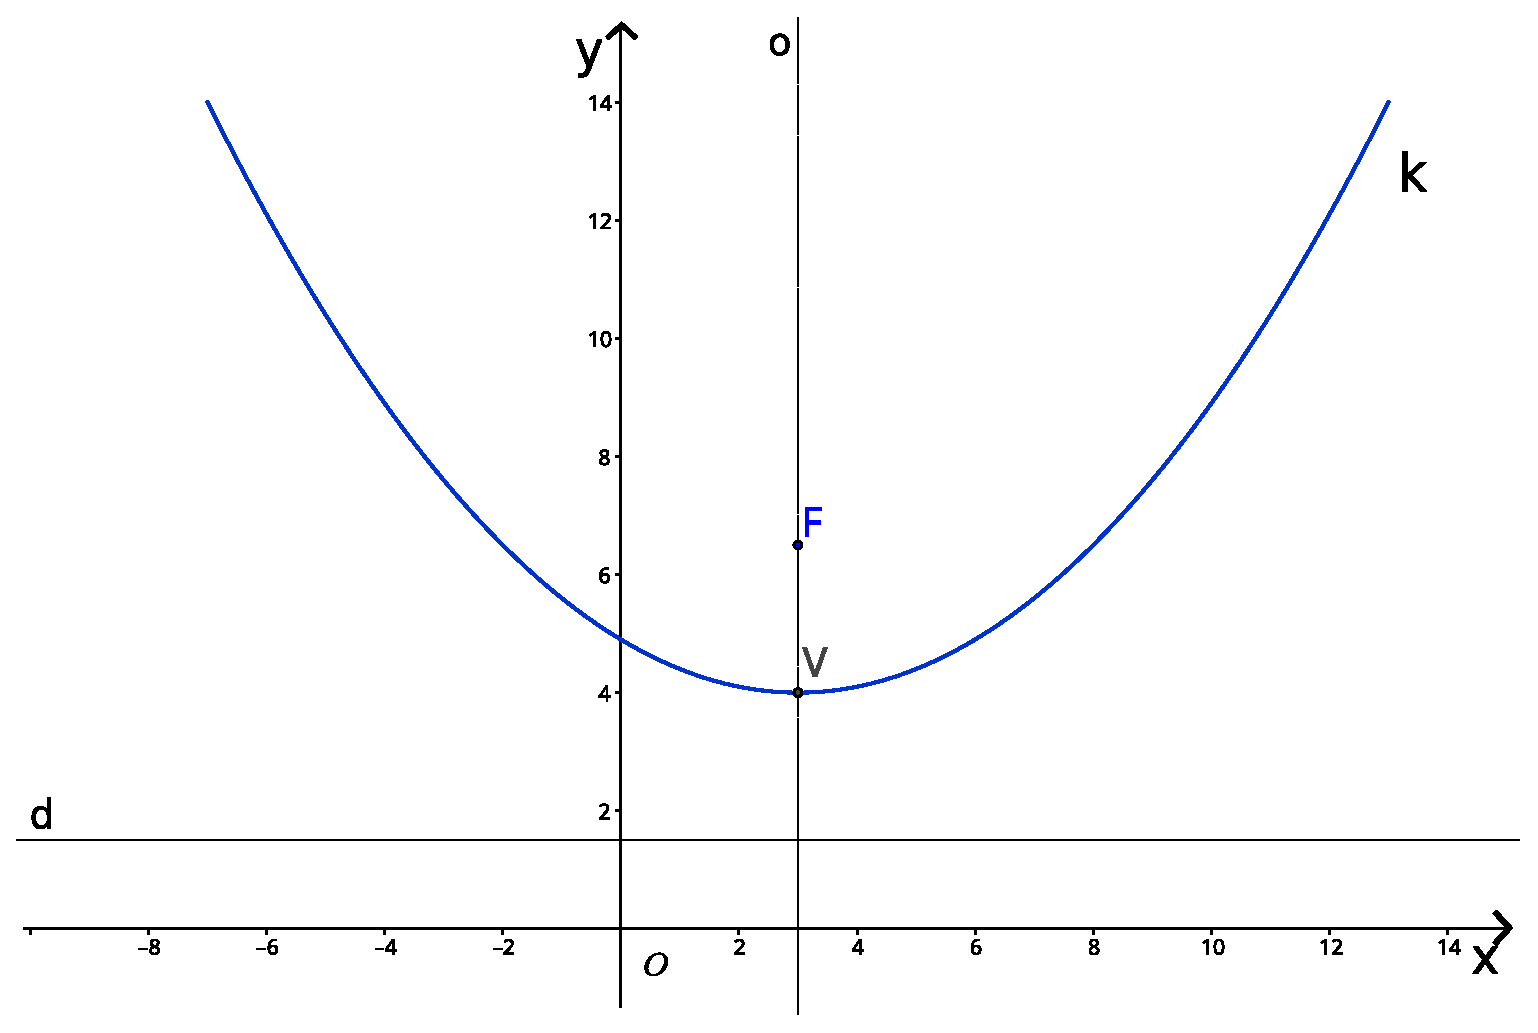
\includegraphics[width=0.8\textwidth]{parabola1.eps}
		      	\caption{Parabola pro $t \in \langle-10, 10\rangle$}
		      \end{figure}
		      				
		      \item
		      Souřadnice bodů \textit{P} a \textit{Q} můžeme vypočítat z obecné rovnice nebo z parametrického vyjádření
		      						
		      \noindent\begin{minipage}[t]{0.5\textwidth}
		      \begin{align*}
		      	x^2-6x-10\cdot\frac{13}{2}+49 & =0   \\
		      	x^2-6x-16                     & =0   \\
		      	x_1 = 8,\: x_2                & = -2 \\
		      	x = t+3,\: t                  & =x-3 \\
		      	t_1 = 5,\: t_2                & = -5 
		      \end{align*}
		\end{minipage}
		\begin{minipage}[t]{0.5\textwidth}
			\begin{align*}
				\frac{t^2}{10} + 4 & = \frac{13}{2}  \\
				\frac{t^2}{10}     & = \frac{5}{2}   \\
				t^2                & = 25            \\
				t_1                & = 5,\: t_2 = -5 
			\end{align*}
		\end{minipage}
		Pro parametr \textit{t} vybereme interval $\langle-5,5\rangle$, 
		\begin{align*}
			k(-5) & =\left[-2, \frac{13}{2}\right], \\
			k(5)  & =\left[8,\frac{13}{2}\right].   
		\end{align*}
		\end{enumerate}
		\vfill
		\begin{figure}[H]
			\centering
			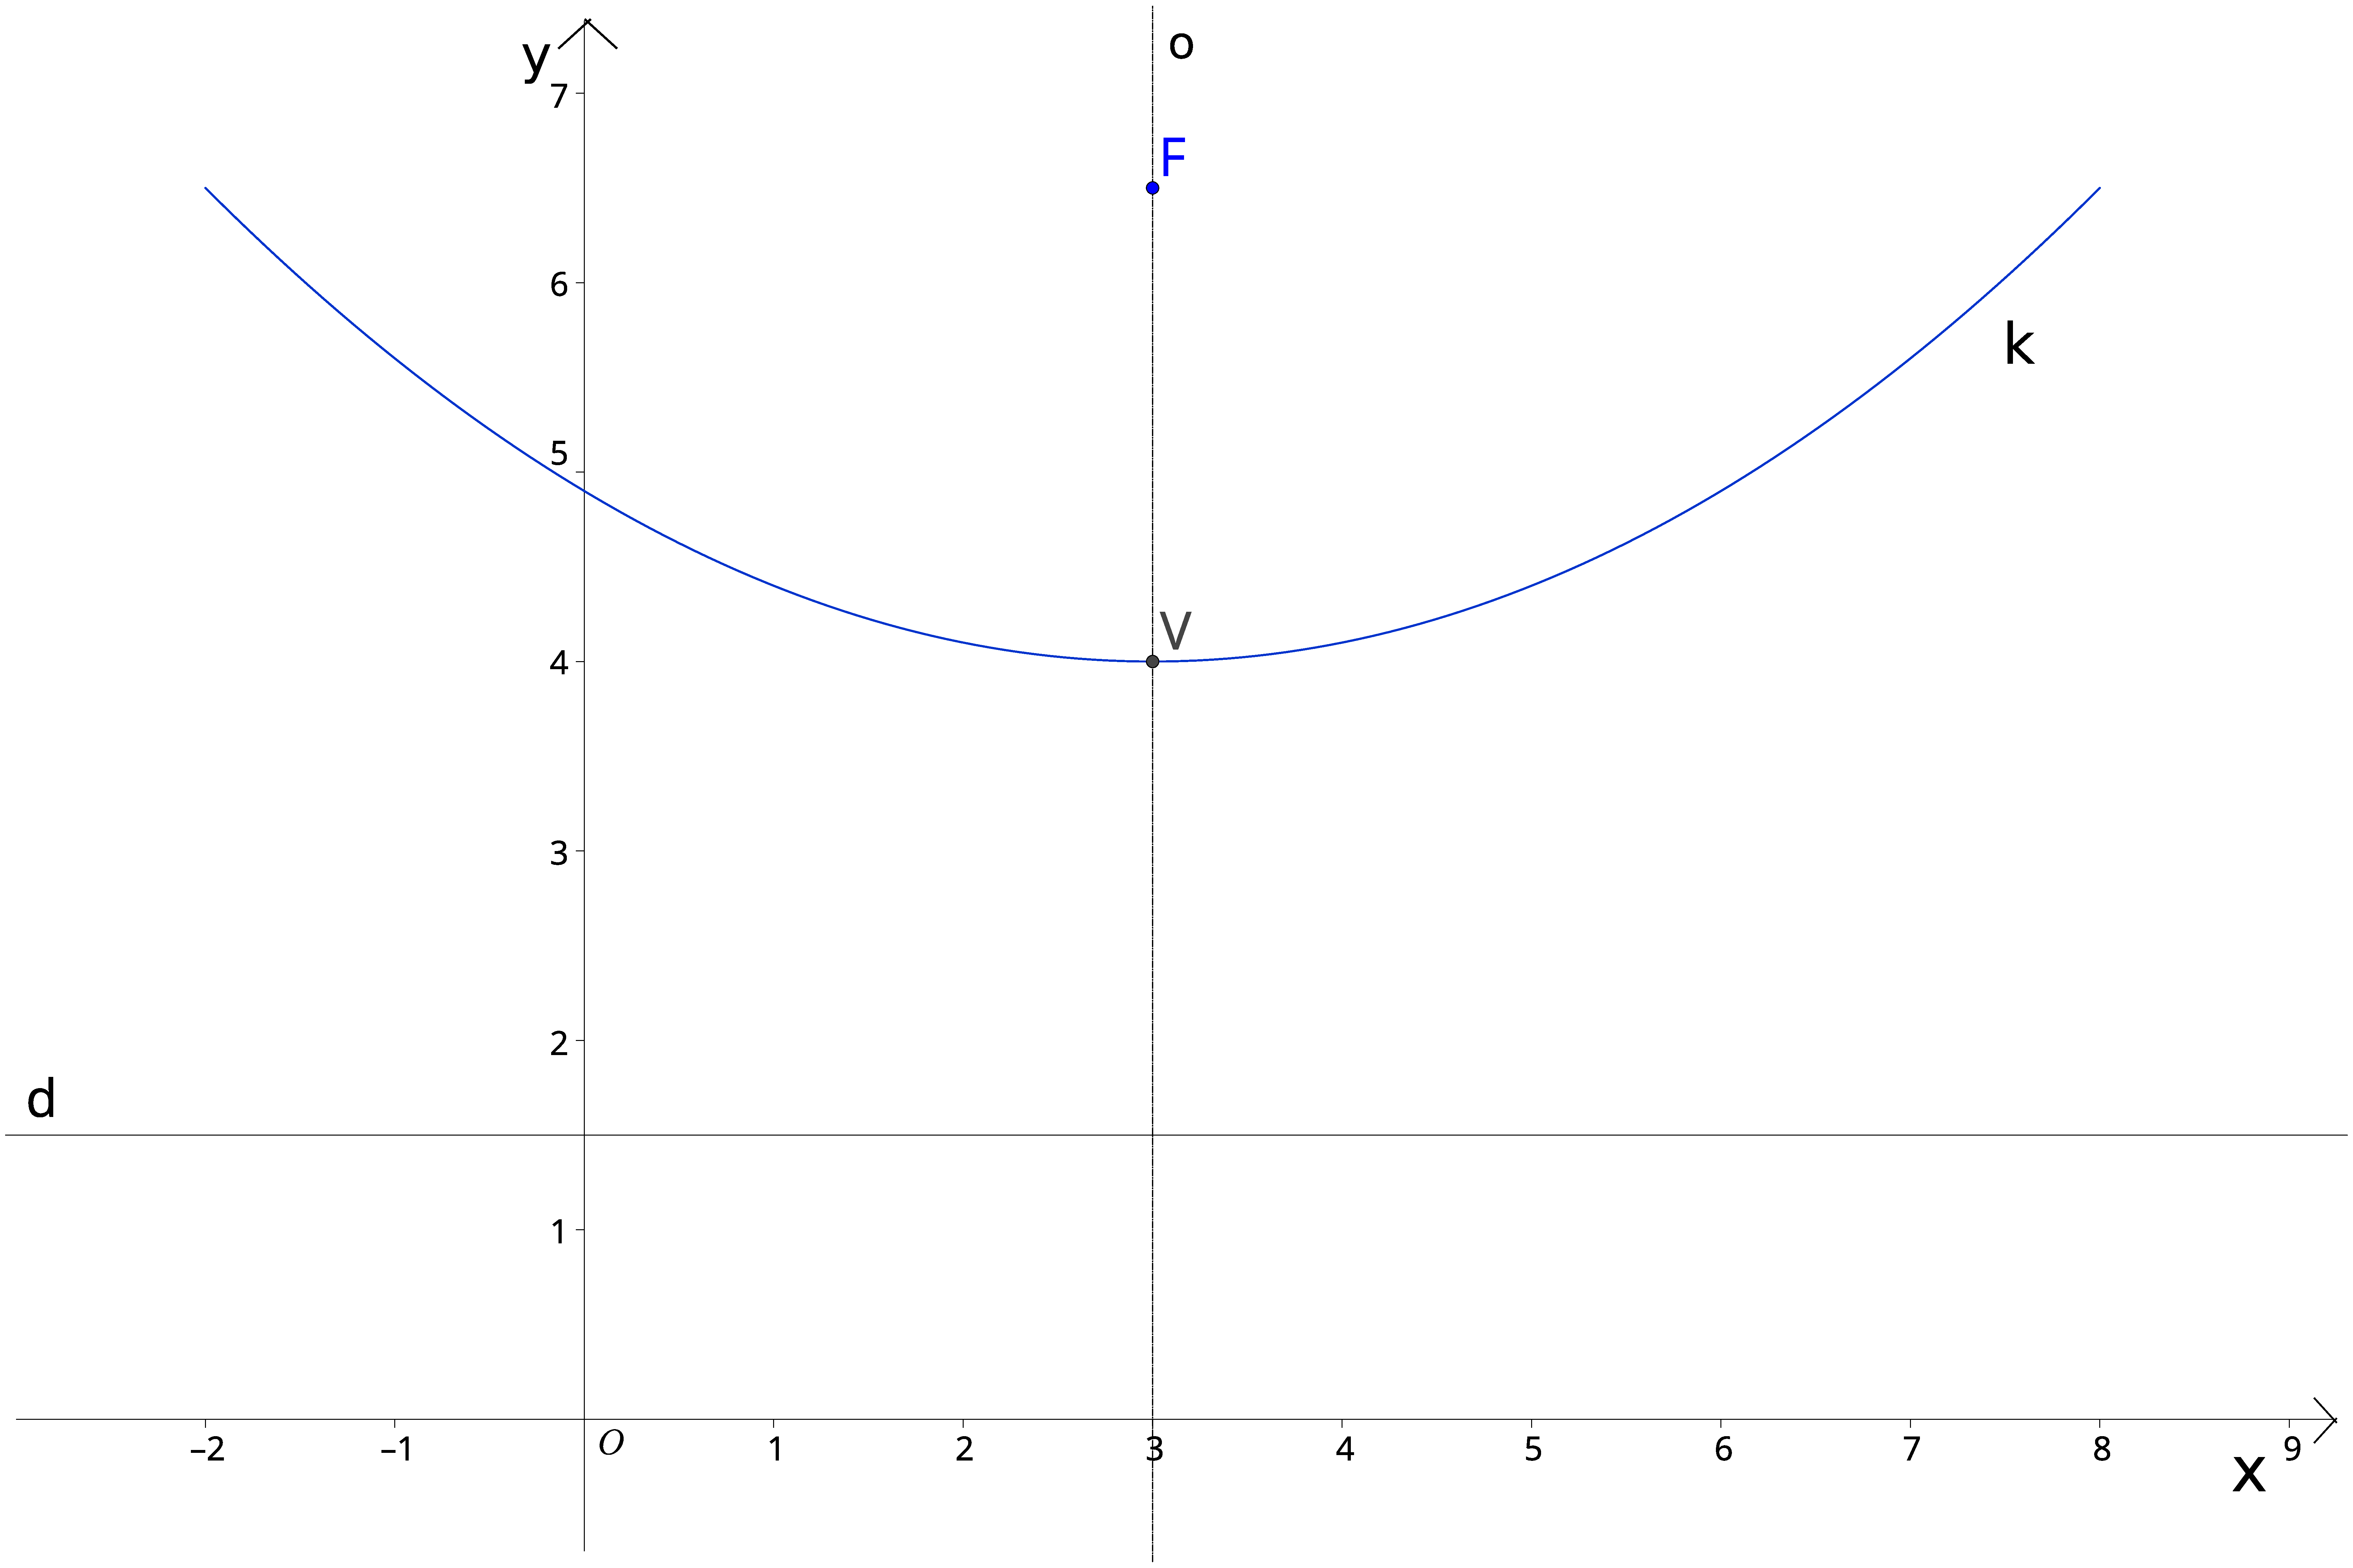
\includegraphics[width=0.9\textwidth]{parabola1-red.eps}
			\caption{Parabola pro $t \in \langle-5, 5\rangle$}					
		\end{figure}
		\clearpage
		\subsection*{Příklad 2}
		Napište parametrické vyjádření paraboly zadané obecnou rovnicí
		$$x^2-6x+10y-31=0.$$
		Napište parametrické vyjádření části paraboly mezi body \textit{P} a \textit{Q}, $x_P = -2$ a $x_Q = 13$.
		Parametrizaci volte tak, aby $k(0) = P$ a část paraboly byla probíhána směrem od bodu \textit{P} do bodu \textit{Q}. \\[5pt]
		\textbf{Řešení:}
		\noindent\begin{enumerate}
		\item Obecnou rovnici upravíme na vrcholový tvar
		$$(x-3)^2=-10(y-4).$$
		Bod $V=[3,4]$ je vrchol, parametr $p=5$, ohnisko $F=\left[3,\frac{3}{2}\right]$,  řídící přímka $d: y=\frac{13}{2}$.
		Volíme $t=x-3$, pak $t^2=-10(y-4)$. Vypočítáme $x=t+3$, $y=-\frac{t^2}{10}+4$.\\
		Parametrické vyjádření paraboly je
		$$k(t)=\left[t+3,-\frac{t^2}{10}+4\right], t \in \mathbb{R}.$$
		\vfill
		\begin{figure}[H]
			\centering
			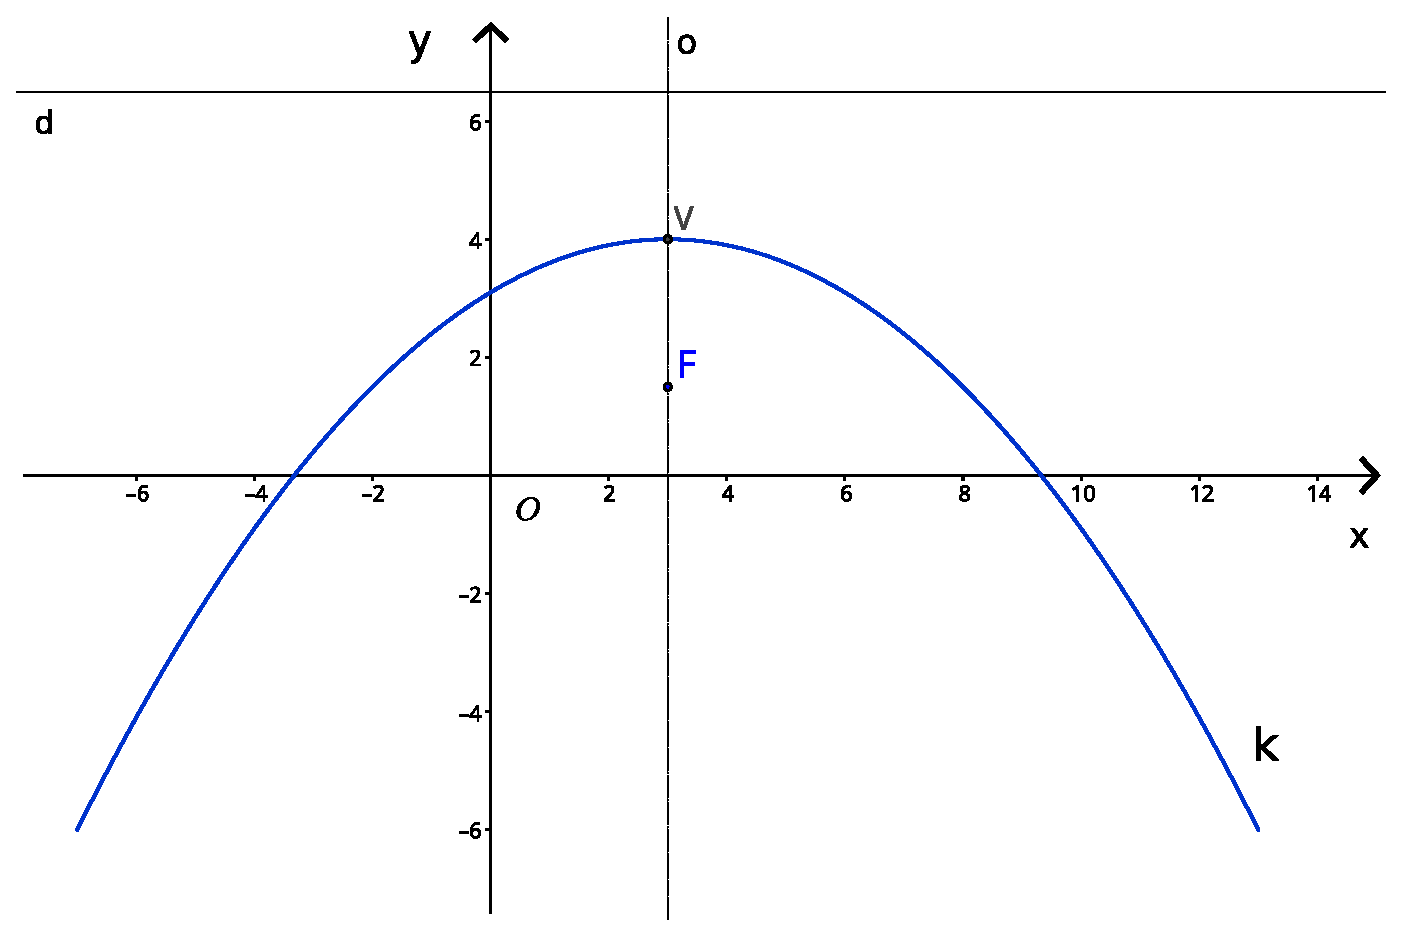
\includegraphics[width=0.8\textwidth]{parabola2.eps}
			\caption{Parabola pro $t \in \langle-10, 10\rangle$}
								
		\end{figure}
		\item
		Interval pro parametrizaci paraboly mezi body \textit{P} a \textit{Q} můžeme vypočítat například z parametrického vyjádření			
								
		\noindent\begin{minipage}[t]{0.5\textwidth}
		\begin{align*}
			t + 3 & = -2 \\
			t_1   & = -5 
		\end{align*}
		\end{minipage}
		\begin{minipage}[t]{0.5\textwidth}
			\begin{align*}
				t + 3 & = 13 \\
				t_2   & = 10 
			\end{align*}
		\end{minipage}
		\\[10pt]
		Daná parabola by tedy byla probíhaná z bodu \textit{P} do bodu \textit{Q} pro parametr \\ $t \in \langle-5, 10\rangle$.
		Aby bylo $k(0) = P$, změníme parametr $t = s - 5$ a máme:
		$$k(s)=\left[s-2,-\frac{(s-5)^2}{10}+4\right], s \in \langle0, 15 \rangle$$
		($s=t+5$, $s_1=-5+5=0$, $s_2=10+5=15$).
		\end{enumerate}
		\vfill
		\begin{figure}[H]
			\centering
			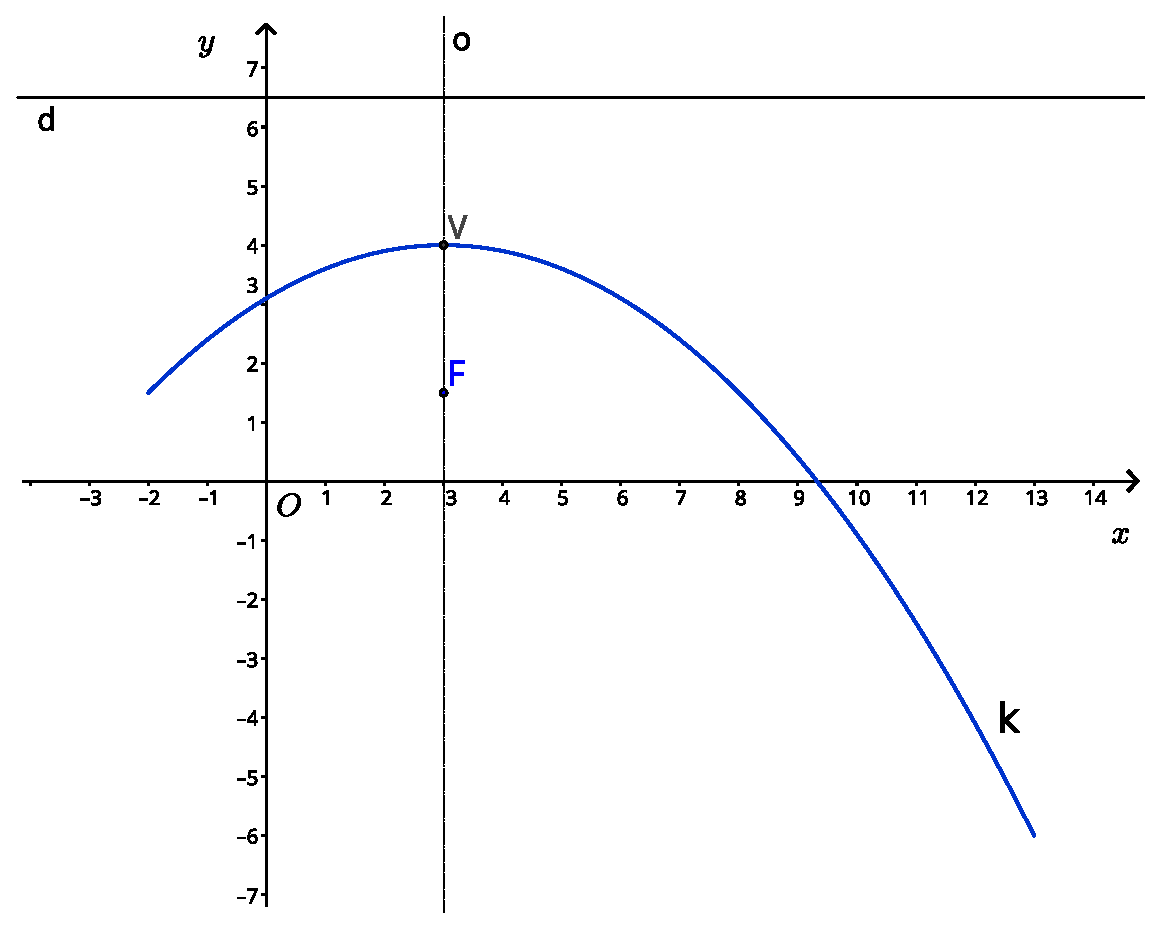
\includegraphics[width=0.9\textwidth]{parabola2-red.eps}
			\caption{Parabola pro $s \in \langle0, 15\rangle$}
								
		\end{figure}
		\clearpage
		\subsection*{Příklad 3}
		Napište parametrické vyjádření paraboly, bod $V=[3,4]$ je vrchol, osa paraboly je rovnoběžná s osou \textit{x} a bod $P=[13,14]$ je bodem paraboly.
		Napište parametrické vyjádření části paraboly mezi bodem \textit{P} a průsečíkem paraboly s osou \textit{x}. \\[5pt]
		\textbf{Řešení:}
		\noindent\begin{enumerate}
		\item Abychom mohli parabolu parametricky vyjádřit, nejdříve napíšeme vrcholový tvar rovnice paraboly.
		Parabola má rovnici $(y-n)^2=2p(x-m)$.
		Dosazením bodů \textit{V}\\ a \textit{P} získáme parametr \textit{p}:
		\begin{align*}
			(14-4)^2 & = 2p(13-3), \\
			100      & = 20p,      \\
			p        & = 5.        
		\end{align*}
		Obecná rovnice paraboly je tedy
		$$(y-4)^2=10(x-3).$$
		Parametr je $p=5$, ohnisko $F=\left[\frac{11}{2},4\right]$,  řídící přímka $d: x=\frac{1}{2}$.\\
		Volíme $t=y-4$, pak $t^2=10(x-3)$. Vypočítáme $x=\frac{t^2}{10}+3$, $y=t+4$.\\
		Parametrické vyjádření paraboly je
		$$k(t) = \left[\frac{t^2}{10}+3, t+4\right], t \in \mathbb{R}.$$
		\vfill
		\begin{figure}[H]
			\centering
			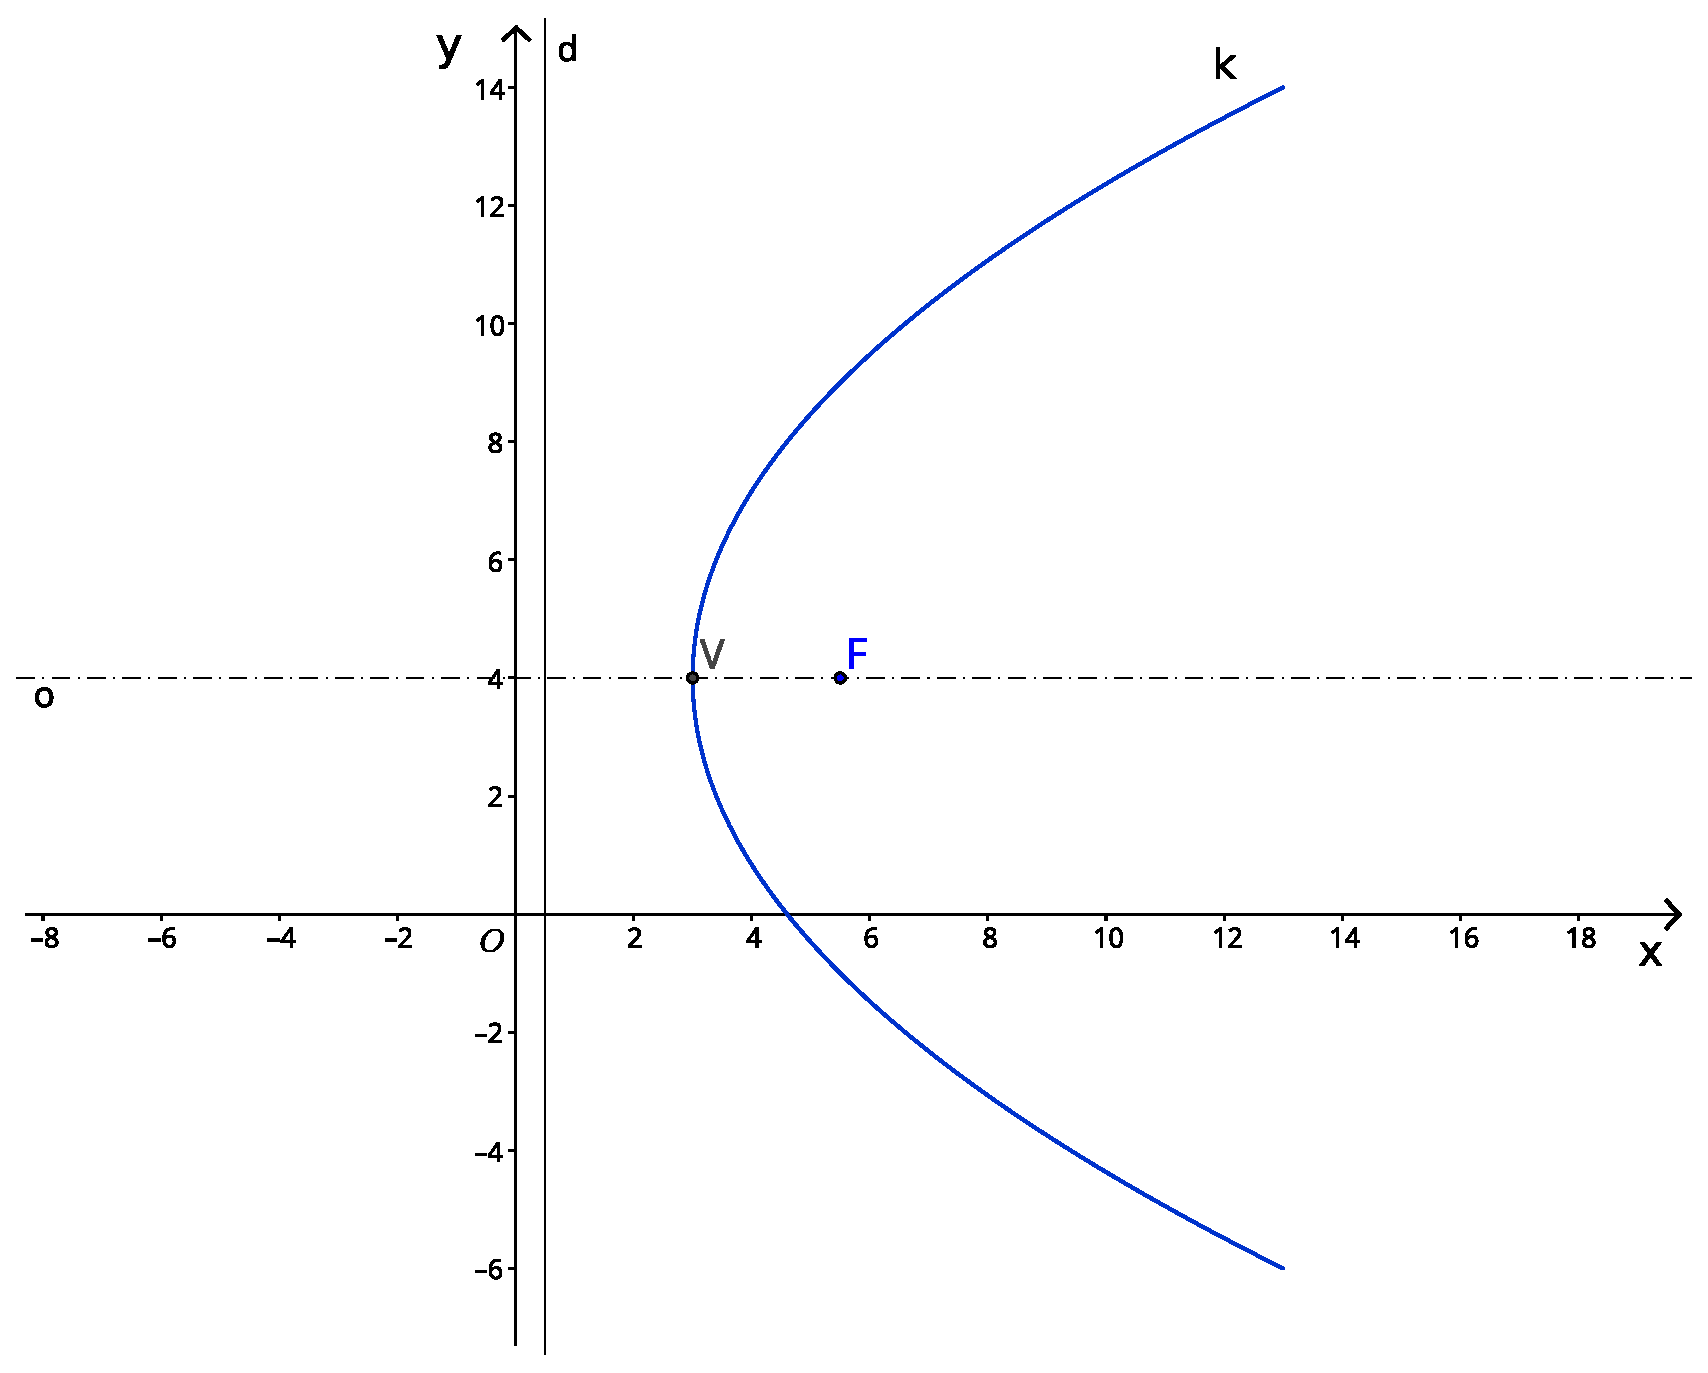
\includegraphics[width=0.5\textwidth]{parabola3.eps}
			\caption{Parabola pro $t \in \langle-10, 10\rangle$}
								
		\end{figure}
		\item
		Hodnoty parametru \textit{t} pro požadovanou část paraboly získáme z rovnic		
									
		\noindent\begin{minipage}[t]{0.5\textwidth}
		\begin{align*}
			t + 4 & = 0 \text{ (průsečík s osou \textit{x})} \\
			t_1   & = -4                                        
		\end{align*}
		\end{minipage}
		\noindent\begin{minipage}[t]{0.5\textwidth}
		\begin{align*}
			t + 4 & = 14 \text{ (bod \textit{P})} \\
			t_2   & = 10                          
		\end{align*}
		\end{minipage}
		\\[10pt]
		Část paraboly mezi bodem \textit{P} a průsečíkem s osou \textit{x} má parametrické vyjádření
		$$k(t) = \left[\frac{t^2}{10}+3, t+4\right], t \in \langle-4, 10\rangle.$$
		\end{enumerate}
		\vfill
		\begin{figure}[H]
			\centering
			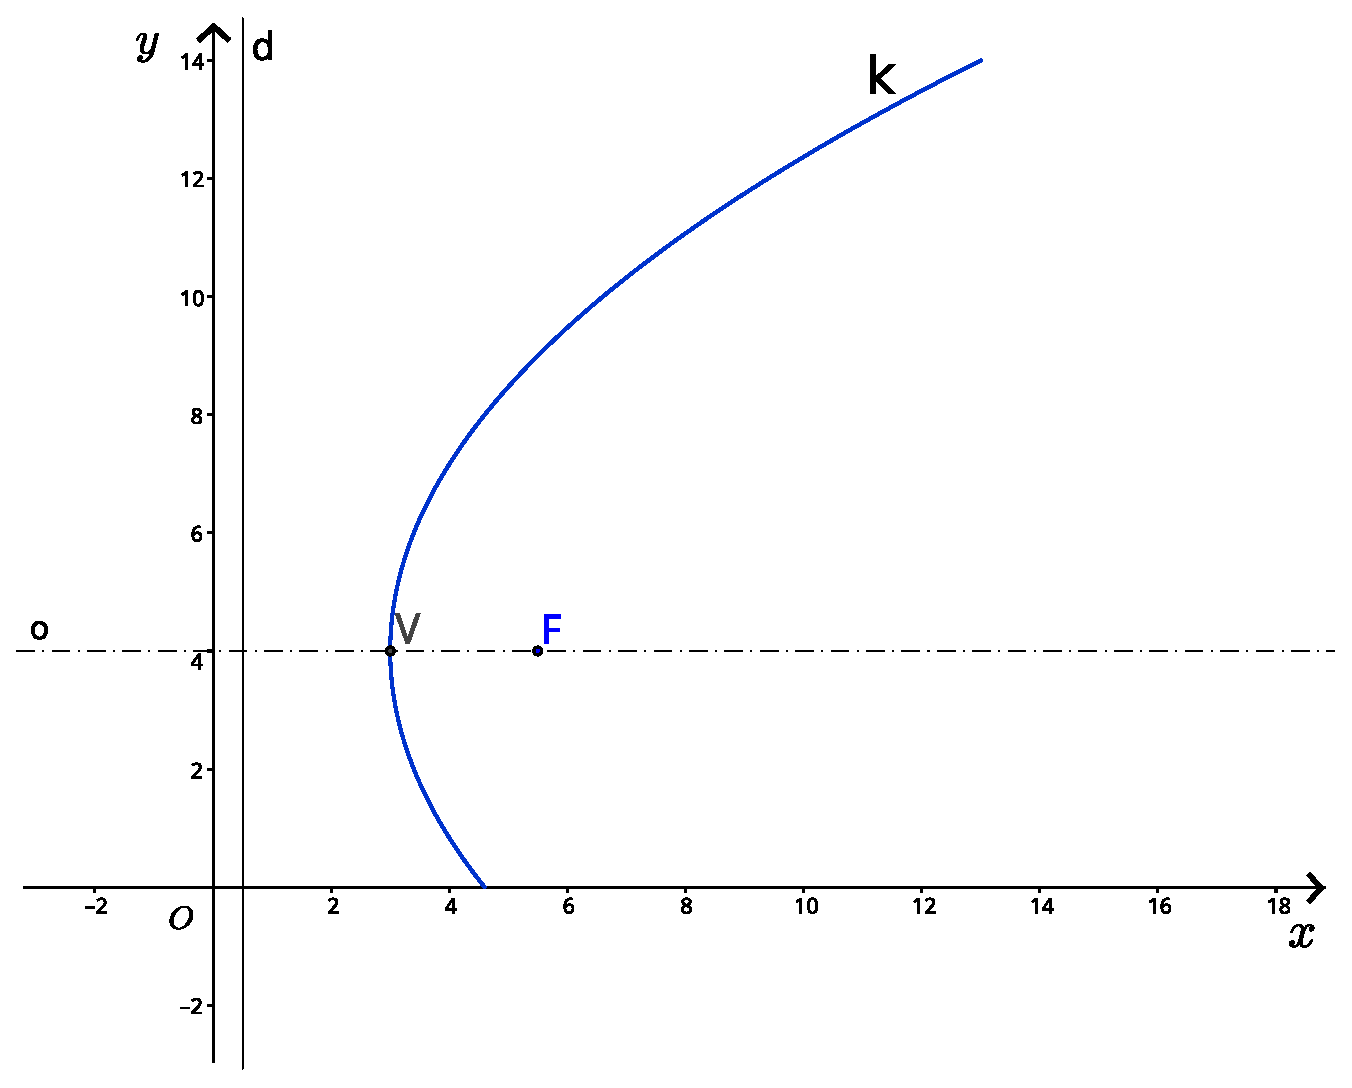
\includegraphics[width=0.9\textwidth]{parabola3-red.eps}
			\caption{Parabola pro $t \in \langle-4, 10\rangle$}
								
		\end{figure}
		\clearpage
		\subsection*{Příklad 4}
		Napište parametrické vyjádření paraboly, bod $F=\left[\frac{1}{2}, 4\right]$ je ohnisko, obecná rovnice
		řídící přímky \textit{d} je $x=\frac{11}{2}$. \\
		Napište parametrické vyjádření části paraboly mezi průsečíkem \textit{P} paraboly s osou \textit{x} a průsečíkem
		\textit{Q} paraboly s osou \textit{y}, $y_Q>0$. \\[5pt]
		\textbf{Řešení:}
		\noindent\begin{enumerate}
		\item Abychom mohli parabolu parametricky vyjádřit, nejdříve napíšeme vrcholový tvar rovnice paraboly.
		Protože řídící přímka je rovnoběžná s osou \textit{y}, je osa paraboly rovnoběžná s osou \textit{x}.
		Parametr \textit{p} je vzdálenost ohniska \textit{F} od řídící přímky \textit{d}, $p=5$. Snadno zjistíme i vrchol $V=[3,4]$. \\
		Parabola má vrcholovou rovnici $(y-n)^2=-2p(x-m)$.
		Po dosazení konkrétních hodnot nám vyjde
		$$(y-4)^2=-10(x-3).$$
		Volíme $t=y-4$, pak $t^2=-10(x-3)$. Vypočítáme $x=-\frac{t^2}{10}+3$, $y=t+4$.\\
		Parametrické vyjádření paraboly je
		$$k(t) = \left[-\frac{t^2}{10}+3, t+4\right], t \in \mathbb{R}.$$
		\vfill
		\begin{figure}[H]
			\centering
			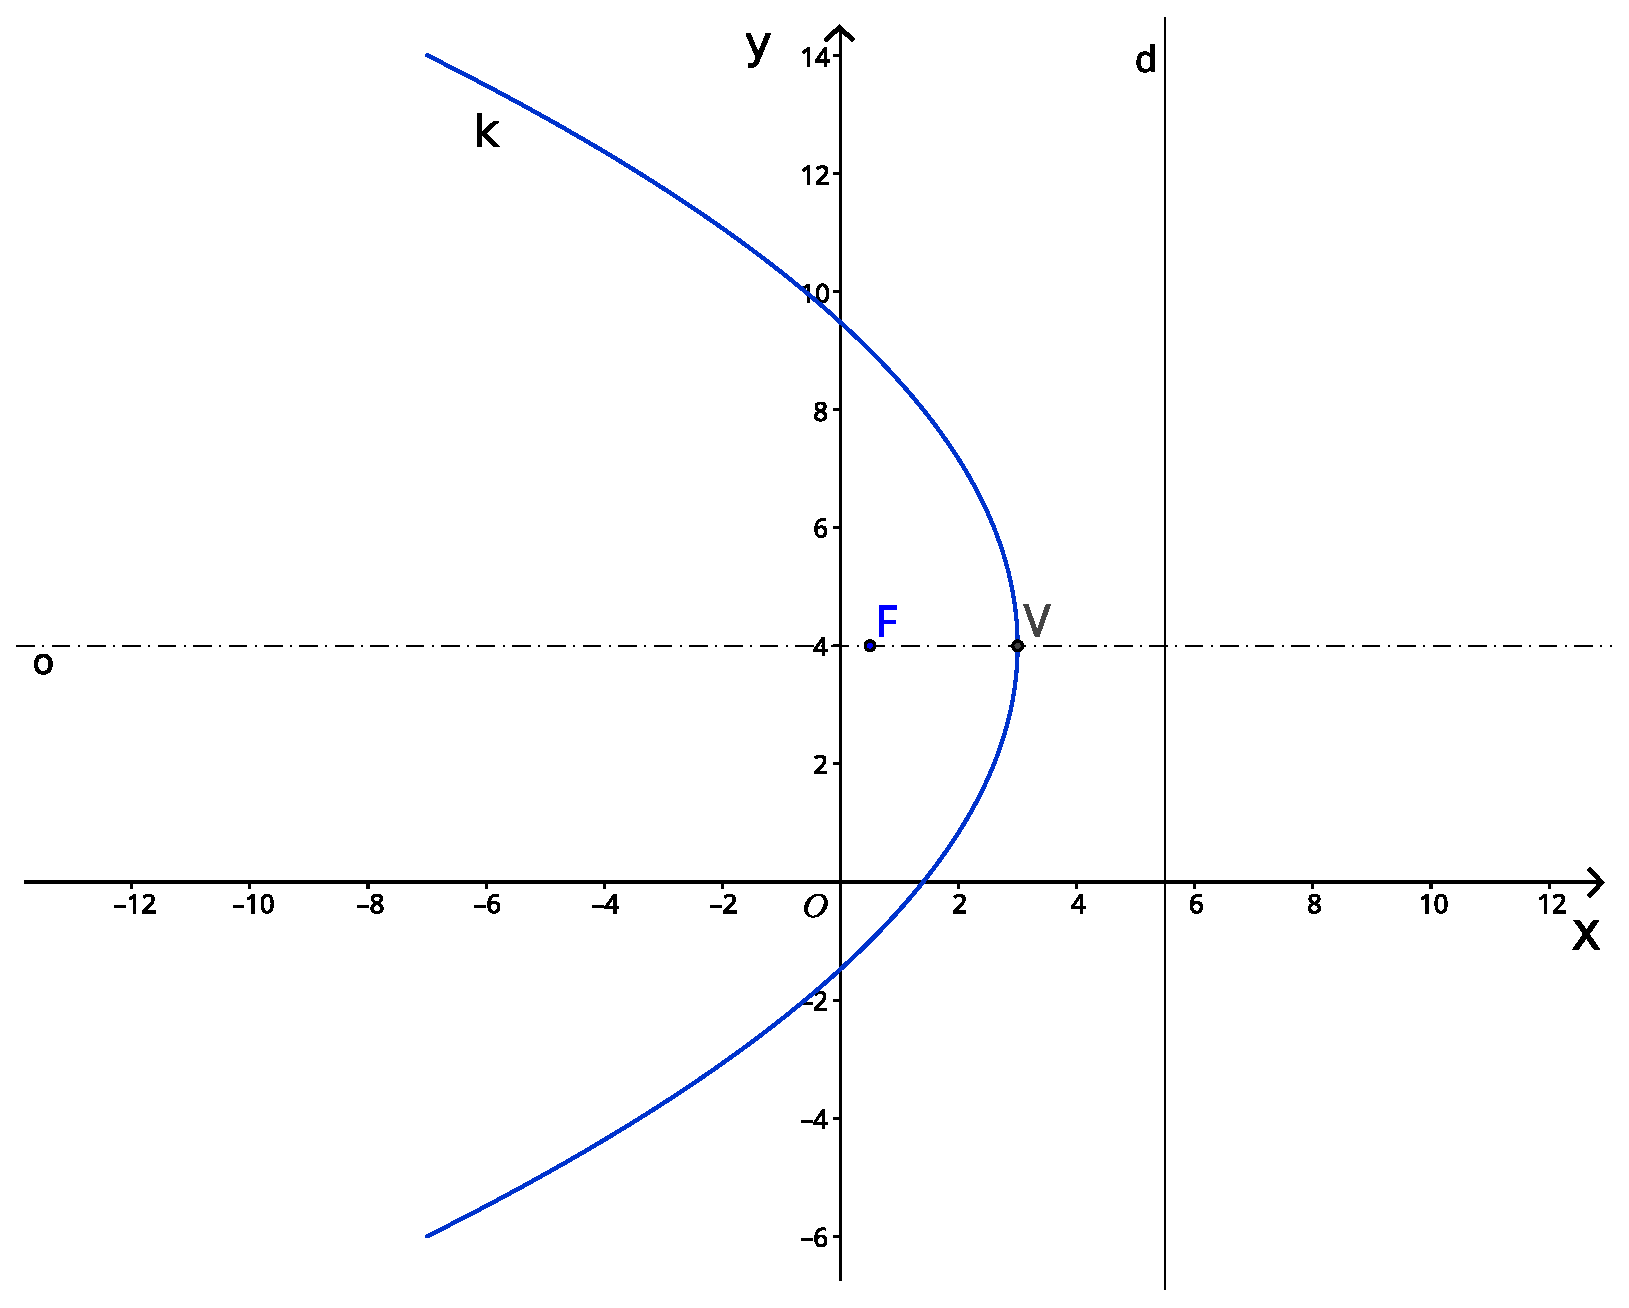
\includegraphics[width=0.7\textwidth]{parabola4.eps}
			\caption{Parabola pro $t \in \langle-10, 10\rangle$}
								
		\end{figure}
		\item
		Hodnoty parametru \textit{t} pro požadovanou část paraboly získáme z rovnic
									
		\noindent\begin{minipage}[t]{0.5\textwidth}
		\begin{align*}
			t + 4 & = 0 \text{ (průsečík s osou \textit{x})} \\
			t_1   & = -4                                        
		\end{align*}
		\end{minipage}
		\noindent\begin{minipage}[t]{0.5\textwidth}
		\begin{align*}
			-\frac{t^2}{10}+3 & = 0 \text{ (bod \textit{Q})} \\
			t^2               & = 30                         \\
			t_2               & = \sqrt{30} \quad (y_Q>0)    
		\end{align*}
		\end{minipage}
		\\[10pt]
		Část paraboly mezi průsečíky \textit{P} a \textit{Q} má vyjádření
		$$k(t) = \left[-\frac{t^2}{10}+3, t+4\right], t \in \langle-4, \sqrt{30}\rangle.$$
		\end{enumerate}
		\vfill
		\begin{figure}[H]
			\centering
			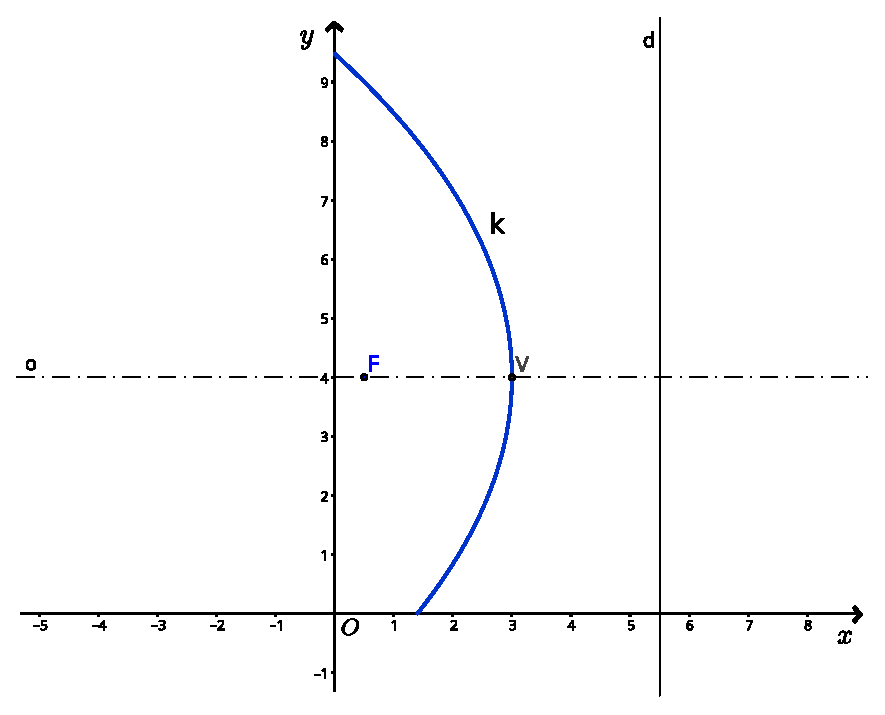
\includegraphics[width=0.9\textwidth]{parabola4-red.eps}
			\caption{Parabola pro $t \in \langle-4, \sqrt{30}\rangle$}
								
		\end{figure}
		\clearpage		
		\section{Elipsa}
		Kružnice je speciální případ elipsy. Dá se předpokládat, že parametrizace elipsy bude podobná parametrizaci kružnice. \\
		Uvažujme nejprve elipsu o středu $O=[0,0]$, velikost hlavní poloosy značíme \textit{a}, velikost vedlejší poloosy
		značíme \textit{b}. Platí $a > b$. \\
		Rovnice elipsy ve středovém tvaru je pak
		$$\frac{x^2}{a^2}+\frac{y^2}{b^2}=1$$
		a hlavní osa elipsy je osa \textit{x}, nebo
		$$\frac{x^2}{b^2}+\frac{y^2}{a^2}=1$$
		a hlavní osa elipsy je osa \textit{y}. \\
		Pro parametrizaci elipsy použijeme vzorec
		$$\cos^2{t}+\sin^2{t}=1.$$
		Pro rovnici $\frac{x^2}{a^2}+\frac{y^2}{b^2}=1$ dáme do rovnosti $\frac{x}{a}=\cos{t}$ a $\frac{y}{b}=\sin{t}$
		(popř. $\frac{x}{a}=\sin{t}$ a $\frac{y}{b}=\cos{t}$). \\
		Parametrický popis elipsy je
		$$k(t)=[a\cos{t}, b\sin{t}]$$
		(popř. $k(t)=[a\sin{t}, b\cos{t}]$), pro jeden oběh bereme $t \in \langle0, 2\pi\rangle$. \\
		Pro rovnici $\frac{x^2}{b^2}+\frac{y^2}{a^2}=1$ dáme do rovnosti $\frac{x}{b}=\cos{t}$ a $\frac{y}{a}=\sin{t}$
		(popř. $\frac{x}{b}=\sin{t}$ a $\frac{y}{a}=\cos{t}$). \\
		Parametrický popis elipsy je
		$$k(t)=[b\cos{t}, a\sin{t}]$$
		(popř. $k(t)=[b\sin{t}, a\cos{t}]$), $t \in \langle0, 2\pi\rangle$. \\
		Snadno ověříme: je-li funkce $\cos$ v \textit{x}-ové souřadnici, výchozí bod $k(0)$ je vrchol na ose \textit{x}, je-li
		funkce $\cos$ v \textit{y}-ové souřadnici, je výchozí bod $k(0)$ vrchol elipsy na ose \textit{y}. \\
		Pro obecnější případ, kdy střed elipsy je bod $S=[m, n]$ a rovnice ve středovém tvaru je
		$$\frac{(x-m)^2}{a^2}+\frac{(y-n)^2}{b^2}=1$$
		nebo
		$$\frac{(x-m)^2}{b^2}+\frac{(y-n)^2}{a^2}=1,$$
		změníme předchozí parametrický popis přičtením vektoru posunutí $S-O=(m,n)$, tedy
		$$k(t)=[m+a\cos{t}, n+b\sin{t}]$$
		(popř. $k(t)=[m+a\sin{t}, n+b\cos{t}]$) \\
		nebo
		$$k(t)=[m+b\cos{t}, n+a\sin{t}].$$
		(popř. $k(t)=[m+b\sin{t}, n+a\cos{t}]$) \\			
		$t \in \langle0, 2\pi\rangle$ pro 1 oběh. \\[10pt]
		Změnou znaménka u funkce $\cos$ měníme výchozí vrchol elipsy, změnou znaménka u funkce $\sin$ měníme směr probíhání elipsy. \\
		Otázka je, zda můžeme vybrat za výchozí bod jiný bod elipsy než vrchol. To je možné, ale museli bychom brát v úvahu sdružené
		průměry elipsy, nebylo by to tak jednoduché jako u kružnice. Tímto se v textu zabývat nebudeme. \\[10pt]
		V této části si ukážeme, jak jednoduše můžeme popsat tečny parametricky zadaných křivek. \\
		Mějme křivku $k(t)=[x(t), y(t)]$, $t \in I$(interval), vybereme si bod na této křivce $K=k(t_0)$ ($t_0$ je vybrané číslo z intervalu \textit{I}).
		Tečna křivky souvisí s derivací, u parametricky zadaných křivek derivujeme zvlášť každou souřadnici a značíme
		$$k'(t)=(x'(t), y'(t)), t \in I.$$
		To jsou tečné vektory křivky \textit{k}. \\
		Tečný vektor v bodě $K=k(t_0)$ je vektor
		$$k'(t_0)=(x'(t_0), y'(t_0)).$$
		Velikost tohoto vektoru vypovídá navíc o rychlosti, jakou je křivka v daném bodě probíhána. Tečna křivky \textit{k} v bodě \textit{K}
		je určena bodem $K=k(t_0)$ a směrovým vektorem $k'(t_0)$.
		\clearpage
		\subsection*{Příklad 1}
		\noindent Napište parametrické vyjádření elipsy zadané obecnou rovnicí
		$$9x^2+16y^2-72x-96y=0.$$
		Dále napište souřadnice průsečíků se souřadnicovými osami a napište obecné rovnice tečen elipsy v těchto  průsečících. \\[10pt]
		\textbf{Řešení:} Obecnou rovnici upravíme na středový tvar
		$$\frac{(x-4)^2}{32}+\frac{(y-3)^2}{18}=1.$$
		Střed elipsy je bod $S=[4,3]$, hlavní osa je rovnoběžná s osou \textit{x}, velikost hlavní poloosy je $a=4\sqrt{2}$,
		velikost vedlejší poloosy $b=3\sqrt{2}$. \\
		Dáme do rovnosti např.
		\begin{align*}
			\frac{x-4}{4\sqrt{2}} & = \cos{t},  \\
			\frac{y-3}{3\sqrt{2}} & = \sin{t} . 
		\end{align*}
		a máme parametrické vyjádření
		$$k(t) = [4+4\sqrt{2} \cdot \cos{t}, 3+3\sqrt{2} \cdot \sin{t}], t\in\langle0,2\pi\rangle.$$
		Výchozí bod je bod $k(0) = [4+4\sqrt{2},3]$, což je pravý hlavní vrchol. Protože $k\left(\frac{\pi}{2}\right) = [4, 3+3\sqrt{2}]$
		je horní vedlejší vrchol, je elipsa probíhána v kladném směru. Souřadnice průsečíků se souřadnicovými osami
		můžeme určit z obecné rovnice nebo z parametrického vyjádření:
		\begin{enumerate}
			\item průsečíky s osou \textit{x} ($y=0$)
			      				      			
			      \noindent\begin{minipage}[t]{0.5\textwidth}
			      \begin{align*}
			      	9x^2-72x & = 0 \\
			      	9x(x-8)  & = 0 \\
			      	x_1      & = 0 \\
			      	x_2      & = 8 \\
			      \end{align*}
			      Průsečíky s osou \textit{x} jsou body $P_1=[0,0]$ a $P_2=[8,0]$.
			\end{minipage}
			nebo
			\noindent\begin{minipage}[t]{0.5\textwidth}
			\begin{align*}
				3+3\sqrt{2}\sin{t}              & = 0                           \\
				\sin{t}                         & = -\frac{\sqrt{2}}{2}         \\
				t_1                             & = \frac{5\pi}{4}              \\
				t_2                             & = \frac{7\pi}{4}              \\
				\text{(vybíráme řešení v } & \langle0, 2\pi\rangle\text{)} \\
				k\left(\frac{5\pi}{4}\right)    & = [0, 0]                      \\
				k\left(\frac{7\pi}{4}\right)    & = [8, 0]                      
			\end{align*}
			\end{minipage}		
			\item průsečíky s osou \textit{y} ($x=0$)
			      				      			
			      \noindent\begin{minipage}[t]{0.5\textwidth}
			      \begin{align*}
			      	16y^2-96y & = 0 \\
			      	16y(y-6)  & = 0 \\
			      	y_1       & = 0 \\
			      	y_2       & = 6 \\
			      \end{align*}
			      Průsečíky s osou \textit{y} jsou body $P_1=[0,0]$ a $P_3=[0,6]$.
			\end{minipage}
			\noindent\begin{minipage}[t]{0.5\textwidth}
			\begin{align*}
				4+4\sqrt{2}\cos{t}           & = 0                   \\
				\cos{t}                      & = -\frac{\sqrt{2}}{2} \\
				t_1                          & = \frac{5\pi}{4}      \\
				t_3                          & = \frac{3\pi}{4}      \\
				k\left(\frac{5\pi}{4}\right) & = [0, 0]              \\
				k\left(\frac{3\pi}{4}\right) & = [0, 6]              
			\end{align*}
			\end{minipage}	
		\end{enumerate}
		Nyní vypočítáme tečné vektory:
		$$k'(t) = (-4\sqrt{2} \cdot \sin{t}, 3\sqrt{2} \cdot \cos{t}).$$
		V bodě $k\left(\frac{5\pi}{4}\right) = [0,0]$ je tečný vektor $k'\left(\frac{5\pi}{4}\right) = (4,-3)$
		a obecná rovnice tečny je \\ $p_1: 3x+4y=0$. \\
		V bodě $k\left(\frac{3\pi}{4}\right) = [0,6]$ je tečný vektor $k'\left(\frac{3\pi}{4}\right) = (-4,-3)$
		a obecná rovnice tečny je \\ $p_3: 3x-4y+24=0$. \\
		V bodě $k\left(\frac{7\pi}{4}\right) = [8,0]$ je tečný vektor $k'\left(\frac{7\pi}{4}\right) = (4,3)$
		a obecná rovnice tečny je \\ $p_2: 3x-4y-24=0$. \\
		Poslední dvě tečny jsou rovnoběžné.
		\vfill
		\begin{figure}[H]
			\centering
			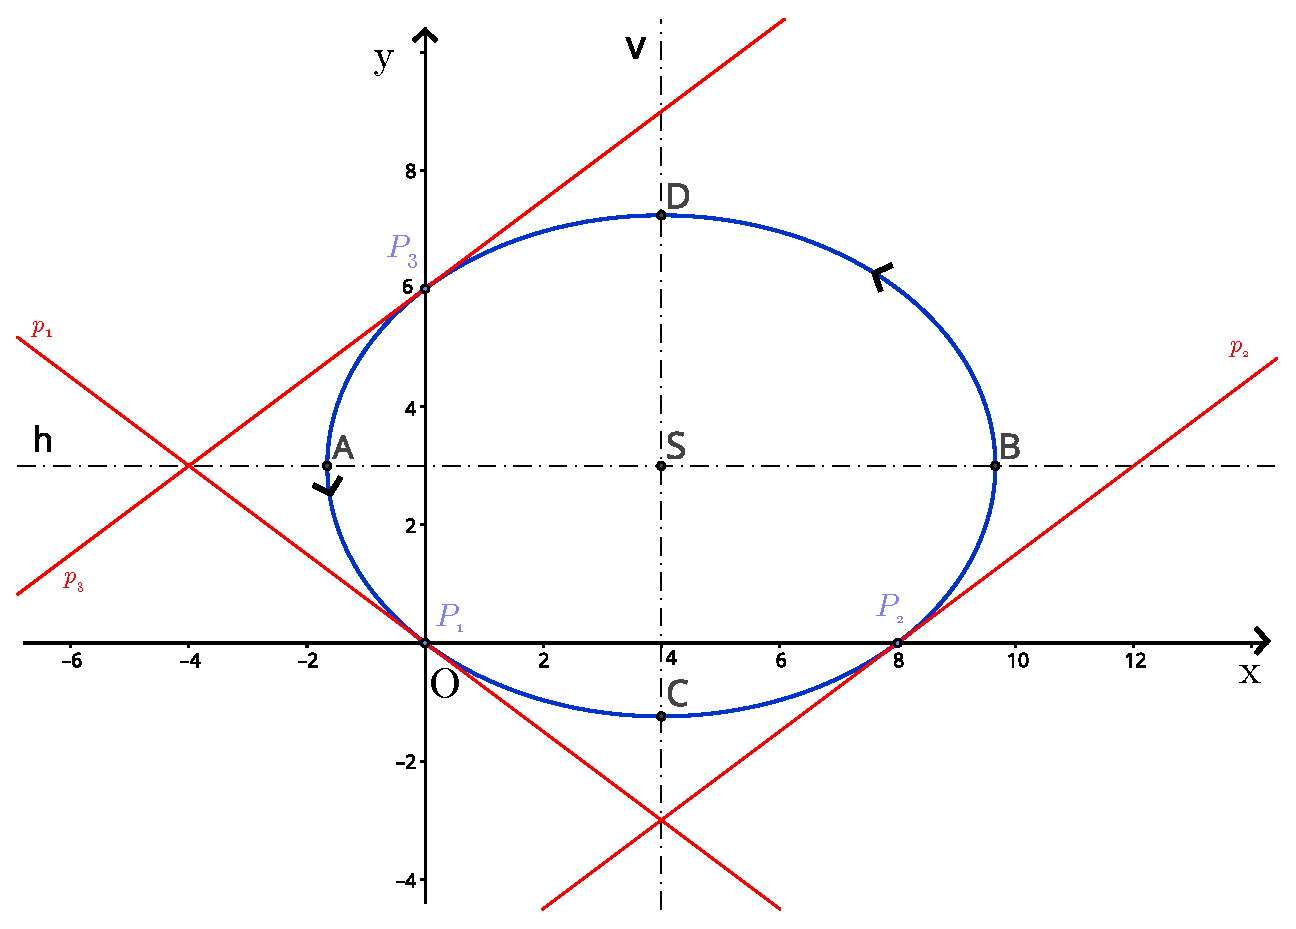
\includegraphics[width=0.9\textwidth]{elipsa1.eps}
			\caption{Elipsa pro $t \in \langle0, 2\pi\rangle$}
								
		\end{figure}
		\clearpage				
		\subsection*{Příklad 2}
		Napište parametrické vyjádření elipsy, body $E=[3,4+\sqrt{14}]$ a $F=[3,4-\sqrt{14}]$ jsou její ohniska,
		velikost vedlejší poloosy $b=3\sqrt{2}$ \\
		Elipsu parametrizujte tak, aby výchozí bod $k(0)$ byl levý vedlejší vrchol a elipsa byla probíhána v kladném směru. \\
		Napište obecné rovnice normál elipsy v jejich průsečících se souřadnými osami. \\
		\textbf{Poznámka:} Normála křivky v bodě \textit{K} je přímka kolmá k tečně v tomto bodě \textit{K}. \\[10pt]
		\textbf{Řešení:} Ze zadaných ohnisek snadno získáme excentricitu $e=\sqrt{14}$ a pomocí vztahu $a^2=e^2+b^2$
		dopočítáme velikost hlavní poloosy $a=4\sqrt{2}$. Střed leží ve středu úsečky $EF$ a jeho souřadnice jsou tedy $S=[3,4]$.\\
		Hlavní osa je rovnoběžná s osou \textit{y}. Vypočítané hodnoty použijeme
		pro napsání středového tvaru obecné rovnice elipsy:
		$$\frac{(x-m)^2}{b^2}+\frac{(y-n)^2}{a^2}=1,$$
		$$\frac{(x-3)^2}{18}+\frac{(y-4)^2}{32}=1.$$
		Pro parametrizaci dáme do rovnosti např.:
		\begin{align*}
			\frac{x-3}{3\sqrt{2}} & = \cos{t}, \\
			\frac{y-4}{4\sqrt{2}} & = \sin{t}. 
		\end{align*}
		a máme parametrické vyjádření
		$$k(t) = [3+3\sqrt{2} \cdot \cos{t}, 4+4\sqrt{2} \cdot \sin{t}], t\in\langle0,2\pi\rangle.$$
		Výchozí bod je bod $k(0) = [3+3\sqrt{2},4]$, což je pravý vedlejší vrchol. Abychom napsali vyjádření s výchozím bodem v
		levém vedlejším vrcholu, změníme znaménko u funkce $\cos$. Protože je $k\left(\frac{\pi}{2}\right)=[3,4+4\sqrt{2}]$, je elipsa probíhána v záporném směru. Změníme tedy i znaménko u funkce $\sin$. \\ Požadované parametrické vyjádření elipsy je pak
		$$k(t) = [3-3\sqrt{2} \cdot \cos{t}, 4-4\sqrt{2} \cdot \sin{t}], t\in\langle0,2\pi\rangle.$$
		Souřadnice průsečíků se souřadnicovými osami
		můžeme určit například z parametrického vyjádření:
		\clearpage
		\begin{enumerate}
			\item průsečíky s osou \textit{x} ($y=0$)
			      				      		
			      \begin{align*}
			      	4-4\sqrt{2}\sin{t}              & = 0                           \\
			      	\sin{t}                         & = \frac{\sqrt{2}}{2}          \\
			      	t_1                             & = \frac{\pi}{4}               \\
			      	t_2                             & = \frac{3\pi}{4}              \\
			      	\text{(vybíráme řešení v } & \langle0, 2\pi\rangle\text{)} \\
			      	k\left(\frac{\pi}{4}\right)     & = [0, 0] = P_1                \\
			      	k\left(\frac{3\pi}{4}\right)    & = [6, 0] = P_2                
			      \end{align*}
			      				      			
			\item průsečíky s osou \textit{y} ($x=0$)
			      				      			
			      \begin{align*}
			      	3-3\sqrt{2}\cos{t}           & = 0                  \\
			      	\cos{t}                      & = \frac{\sqrt{2}}{2} \\
			      	t_1                          & = \frac{\pi}{4}      \\
			      	t_3                          & = \frac{7\pi}{4}     \\
			      	k\left(\frac{\pi}{4}\right)  & = [0, 0] = P_1       \\
			      	k\left(\frac{7\pi}{4}\right) & = [0, 8] = P_3       
			      \end{align*}
		\end{enumerate}
		Nyní vypočítáme tečné vektory
		$$k'(t) = (3\sqrt{2} \cdot \sin{t}, -4\sqrt{2} \cdot \cos{t})$$
		V bodě $k\left(\frac{\pi}{4}\right) = [0,0]$ je tečný vektor $k'\left(\frac{\pi}{4}\right) = (3,-4)$
		a obecná rovnice normály je \\ $n_1: 3x-4y=0$. \\
		V bodě $k\left(\frac{3\pi}{4}\right) = [6,0]$ je tečný vektor $k'\left(\frac{3\pi}{4}\right) = (3,4)$
		a obecná rovnice normály je $n_2: 3x+4y-18=0$. \\
		V bodě $k\left(\frac{7\pi}{4}\right) = [0,8]$ je tečný vektor $k'\left(\frac{7\pi}{4}\right) = (-3,-4)$
		a obecná rovnice normály je $n_3: 3x+4y-32=0$. \\
		\vfill
		\begin{figure}[H]
			\centering
			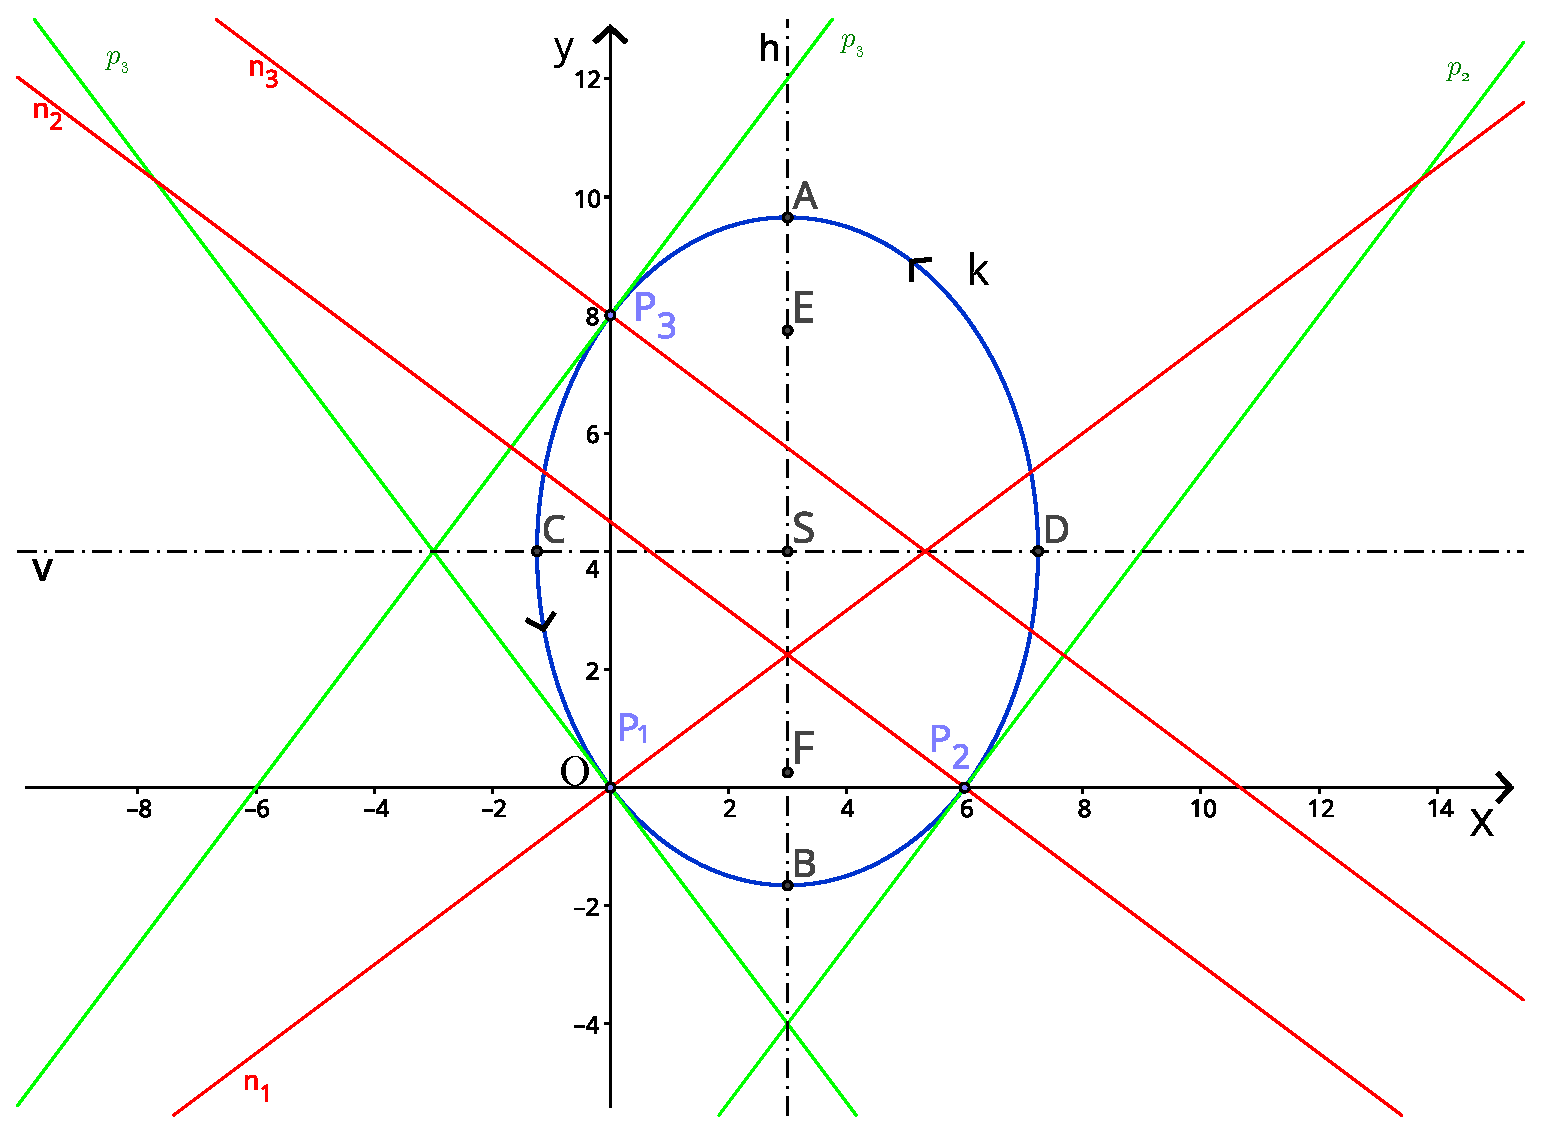
\includegraphics[width=0.9\textwidth]{elipsa2.eps}
			\caption{Elipsa pro $t \in \langle0, 2\pi\rangle$}
								
		\end{figure}
		\clearpage						
		\section{Hyperbola}
		Uvažujme hyperbolu o středu $O=[0,0]$, osy hyperboly jsou souřadnicové osy. Rovnice hyperboly ve středovém tvaru je
		$$\frac{x^2}{a^2}-\frac{y^2}{b^2}=1.$$
		hlavní osa je osa \textit{x}, vrcholy jsou body $A=[a, 0]$, $B[-a, 0]$ \\
		nebo
		$$-\frac{x^2}{b^2}+\frac{y^2}{a^2}=1.$$
		hlavní osa je osa \textit{y}, vrcholy jsou body $A=[0, a]$, $B[0, -a]$ \\[10pt]
			Kladné číslo \textit{a} je velikost hlavní poloosy, kladné číslo \textit{b} je velikost vedlejší poloosy.
			\begin{figure}[H]
				\centering
				\begin{subfigure}{0.5\textwidth}
					\centering
					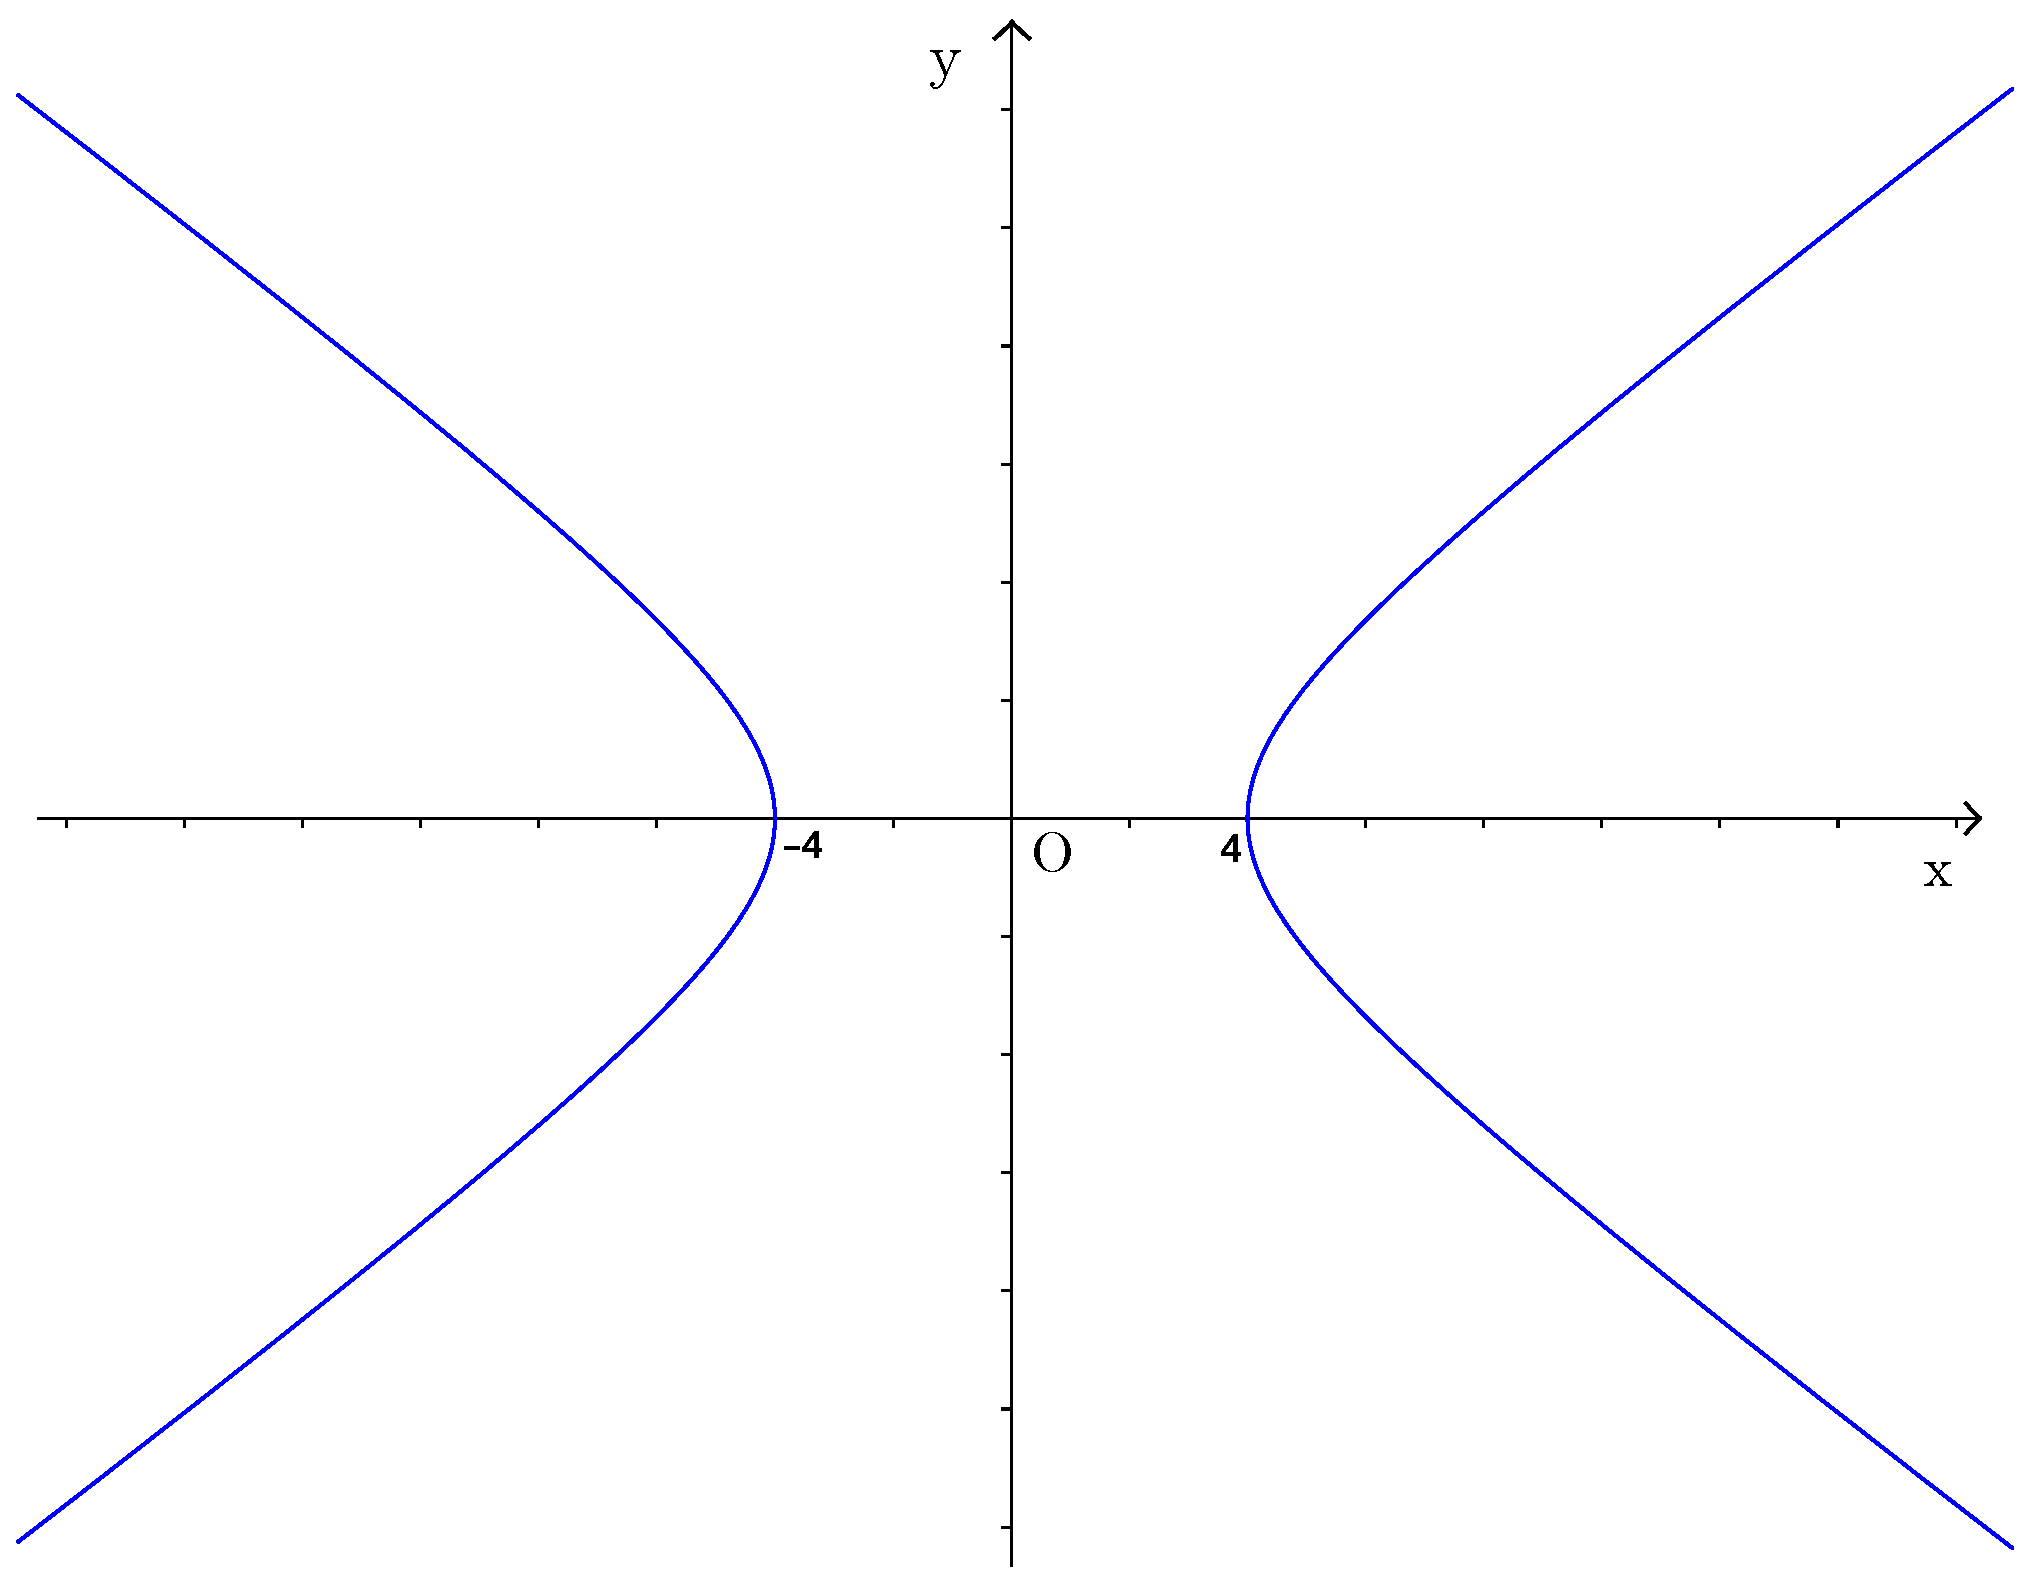
\includegraphics[width=\textwidth]{hyperbola-teorie1a.eps}
					\caption{Hyperbola $\frac{x^2}{16}-\frac{y^2}{9}=1$}
				\end{subfigure}%
				\begin{subfigure}{0.5\textwidth}
					\centering
					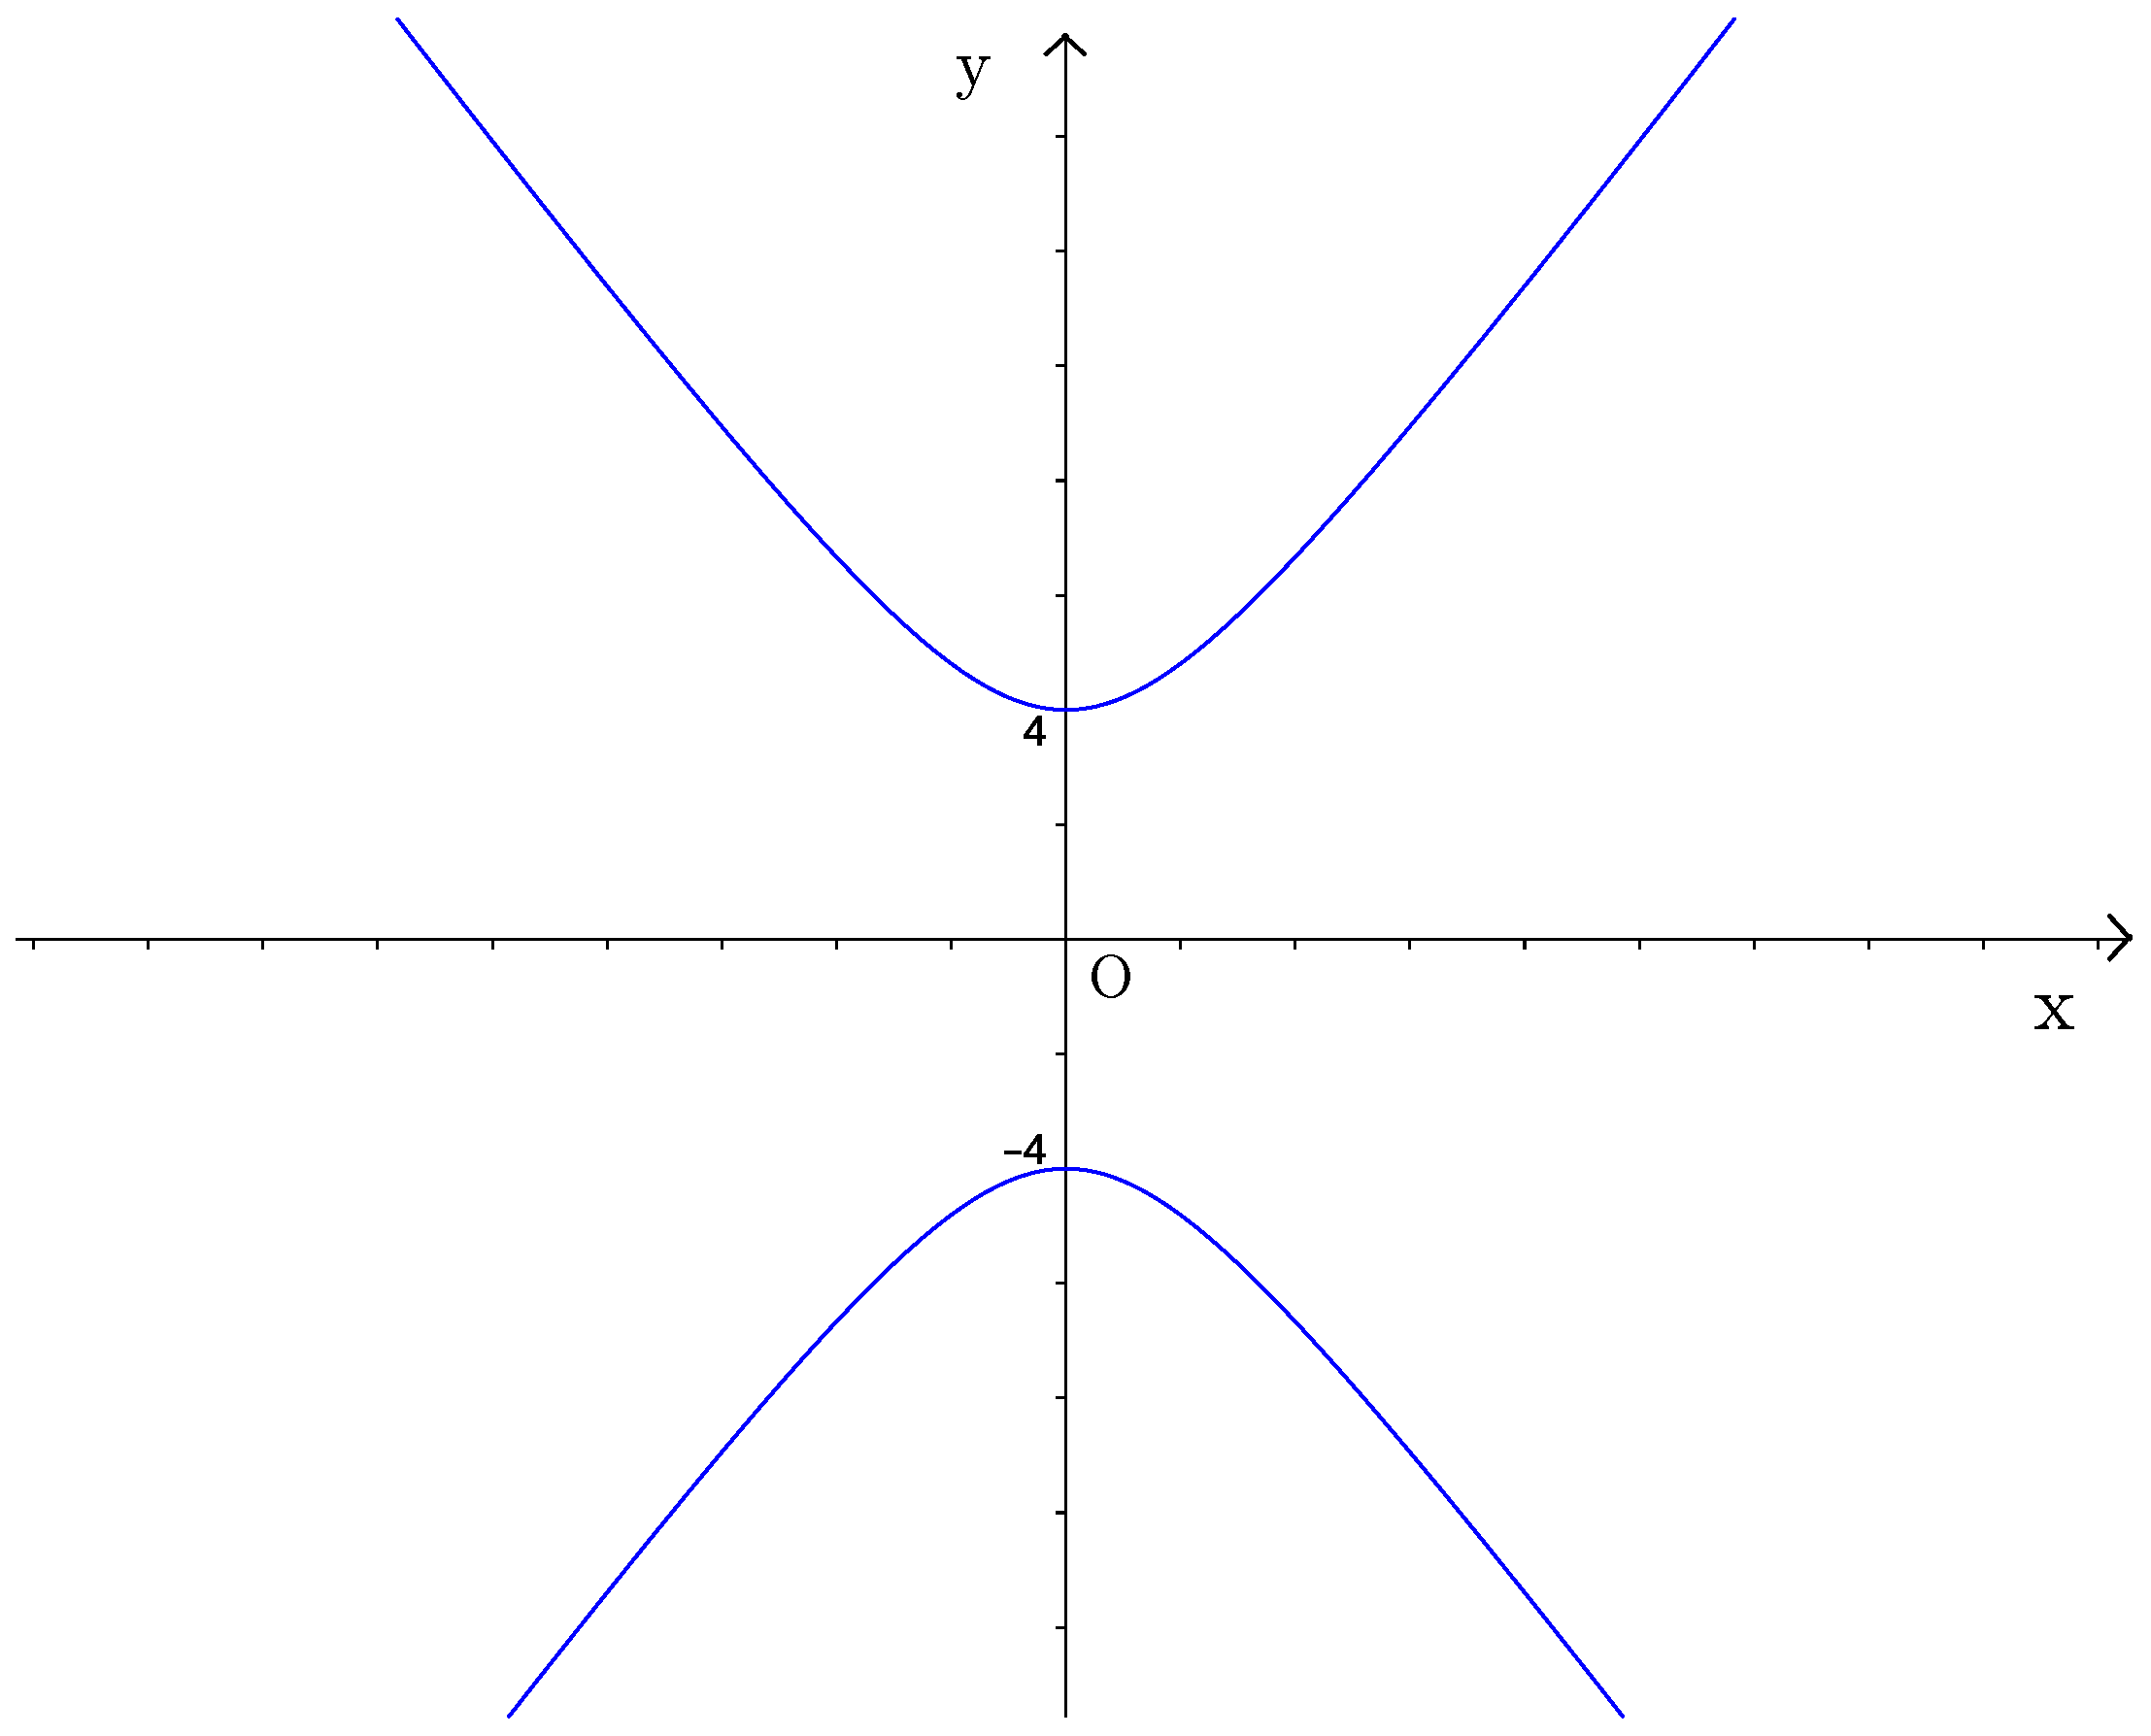
\includegraphics[width=\textwidth]{hyperbola-teorie1b.eps}
					\caption{Hyperbola $-\frac{x^2}{9}+\frac{y^2}{16}=1$}
				\end{subfigure}
				\caption{Hyperboly v základní poloze}
			\end{figure}
			Připomeňme, že může být $a>b$ i $a<b$. Je-li $a=b$, hyperbola se nazývá rovnoosá. Každá hyperbola má 2 tzv. \textit{asymptoty},
			jsou to přímky, ke kterým se tato křivka přibližuje. \\[10pt]
			Pro hyperbolu $\frac{x^2}{a^2}-\frac{y^2}{b^2}=1$ získáme asymptoty z rovnice $\frac{x^2}{a^2}-\frac{y^2}{b^2}=0$, tj.:
			$$\left(\frac{x}{a}-\frac{y}{b}\right)\cdot\left(\frac{x}{a}+\frac{y}{b}\right)=0.$$
			Rovnice asymptot ve směrnicovém tvaru jsou
			$$y=\frac{b}{a}x$$
			a
			$$y=-\frac{b}{a}x.$$
			Pro hyperbolu $-\frac{x^2}{b^2}+\frac{y^2}{a^2}=1$ získáme asymptoty z rovnice $-\frac{x^2}{b^2}+\frac{y^2}{a^2}=0$, tj.:
			$$\left(-\frac{x}{b}+\frac{y}{a}\right)\cdot\left(\frac{x}{b}+\frac{y}{a}\right)=0,$$
			$$y=\frac{a}{b}x$$
			a
			$$y=-\frac{a}{b}x.$$
			\begin{figure}[H]
				\centering
				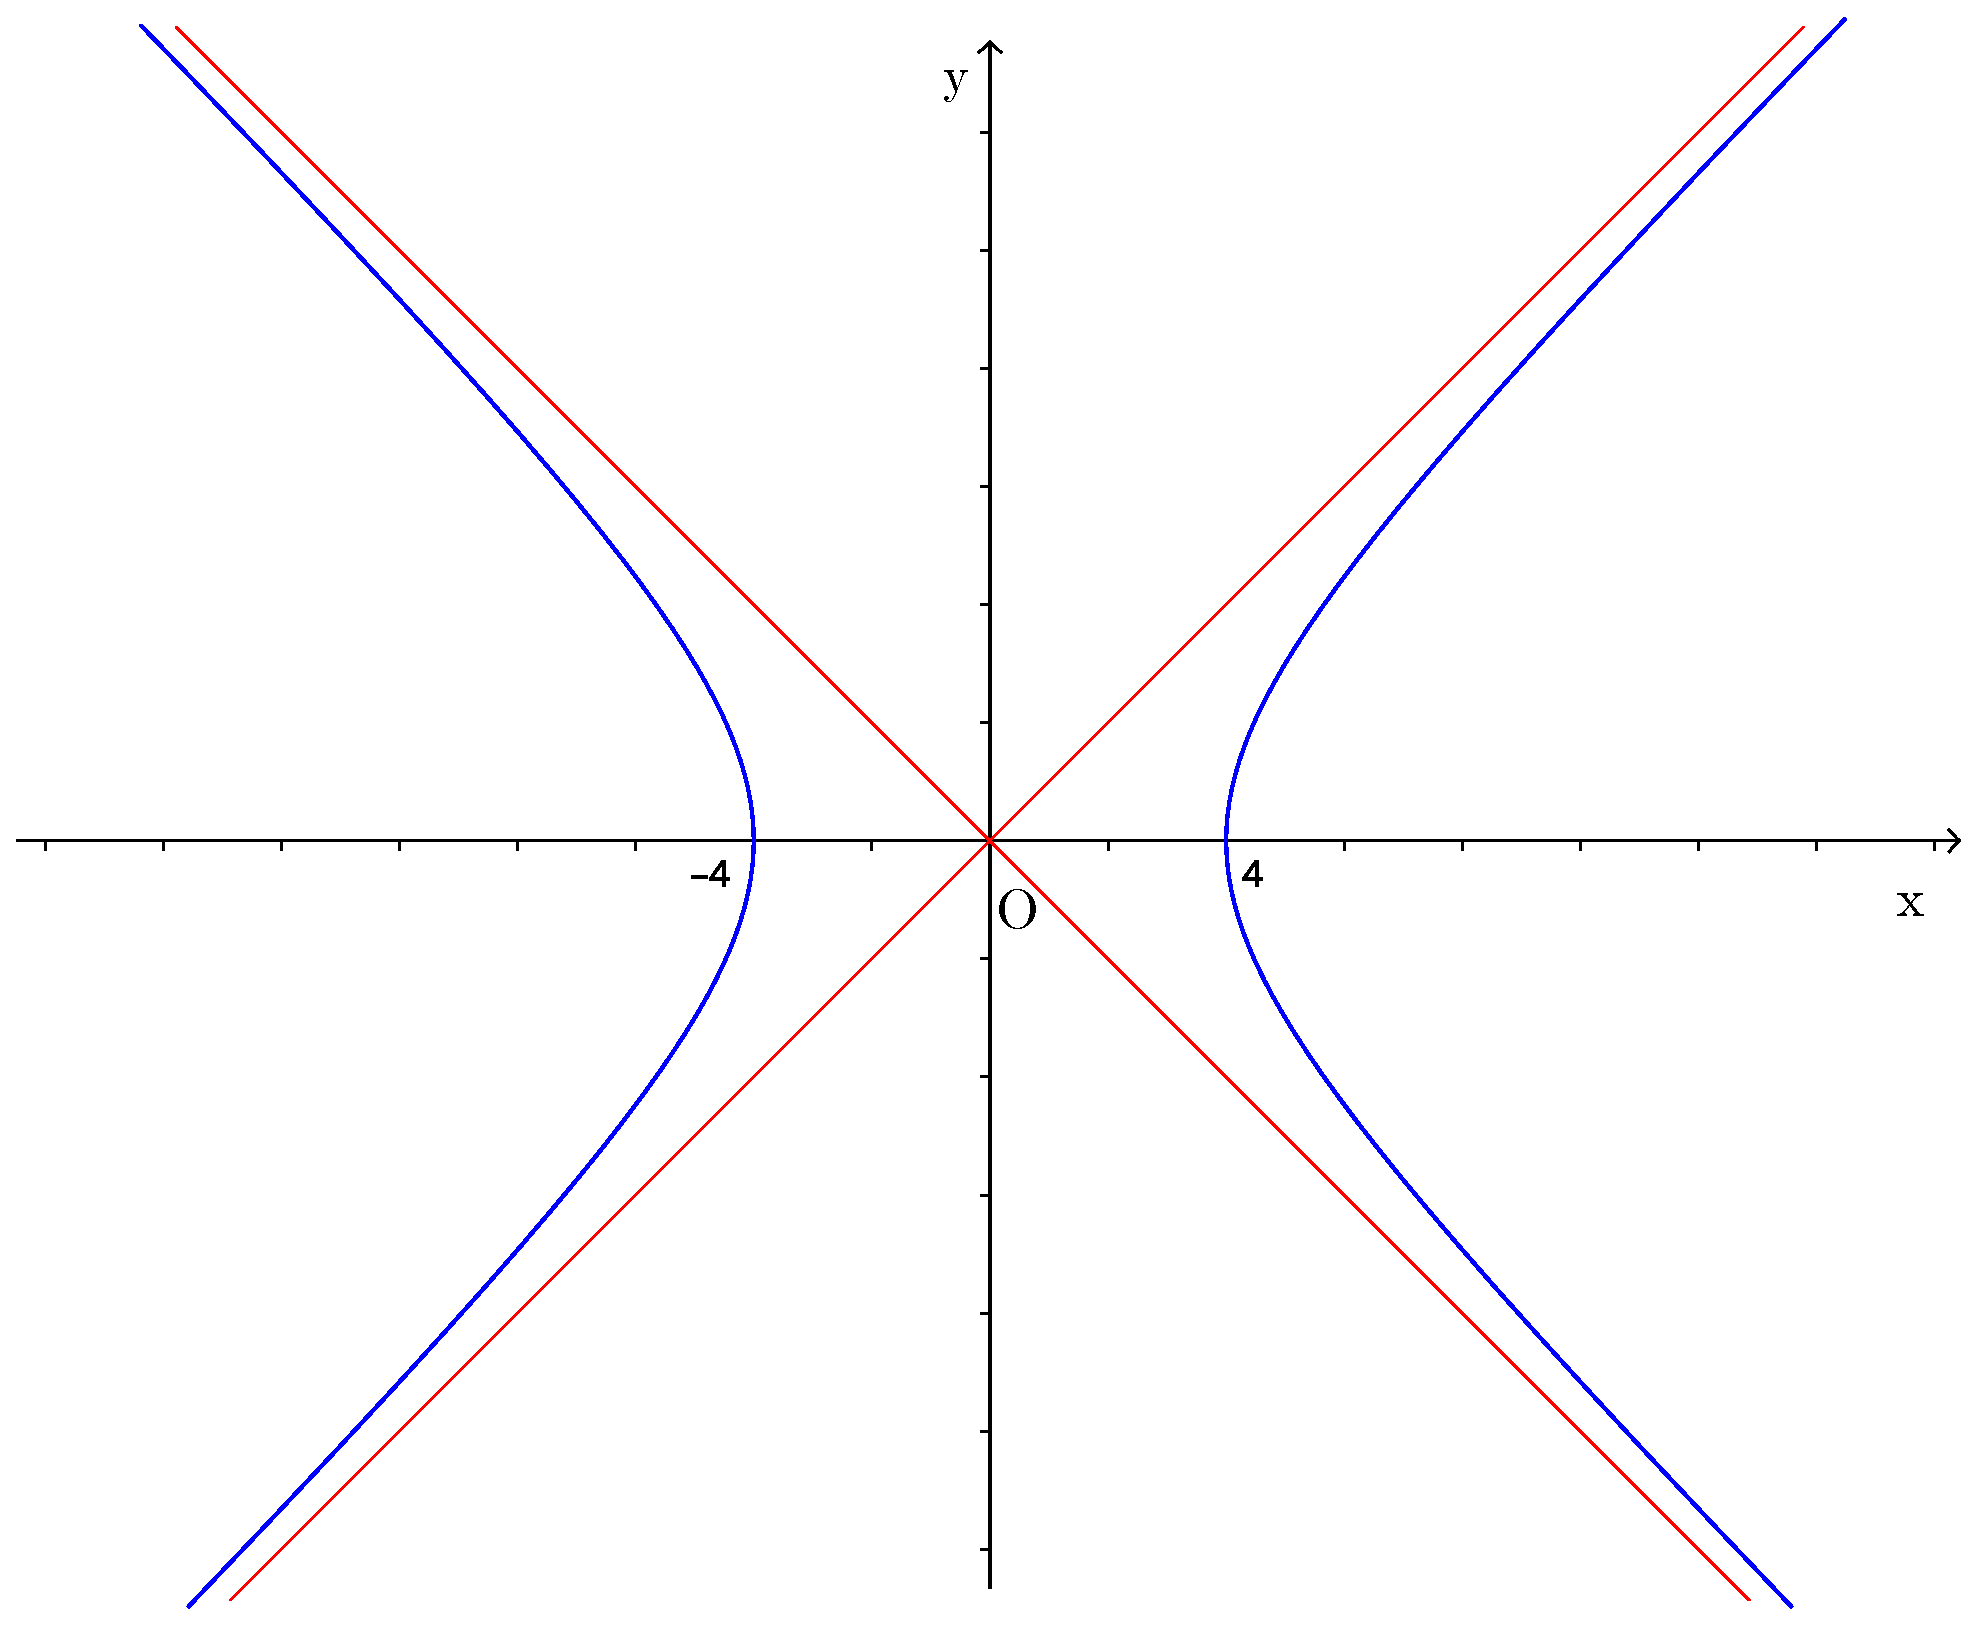
\includegraphics[width=0.75\textwidth]{hyperbola-teorie1c.eps}
				\caption{Asymptoty $y=x$ a $y=-x$ rovnoosé hyperboly $\frac{x^2}{16}-\frac{y^2}{16}=1$}					
			\end{figure}
			Vzhledem k předchozím poznatkům bychom pro parametrizaci hyperboly chtěli najít dvě funkce \textit{f} a \textit{g}, pro které
			by platilo $f^2(t)-g^2(t)=1$. \\[10pt]
			Takové funkce se nazývají hyperbolické a jsou jimi funkce
			$$f(t)=\frac{e^t+e^{-t}}{2}$$
			a
			$$g(t)=\frac{e^t-e^{-t}}{2}.$$
			$D_f=D_g=\mathbb{R}$
			\begin{figure}[H]
				\centering
				\begin{subfigure}{0.5\textwidth}
					\centering
					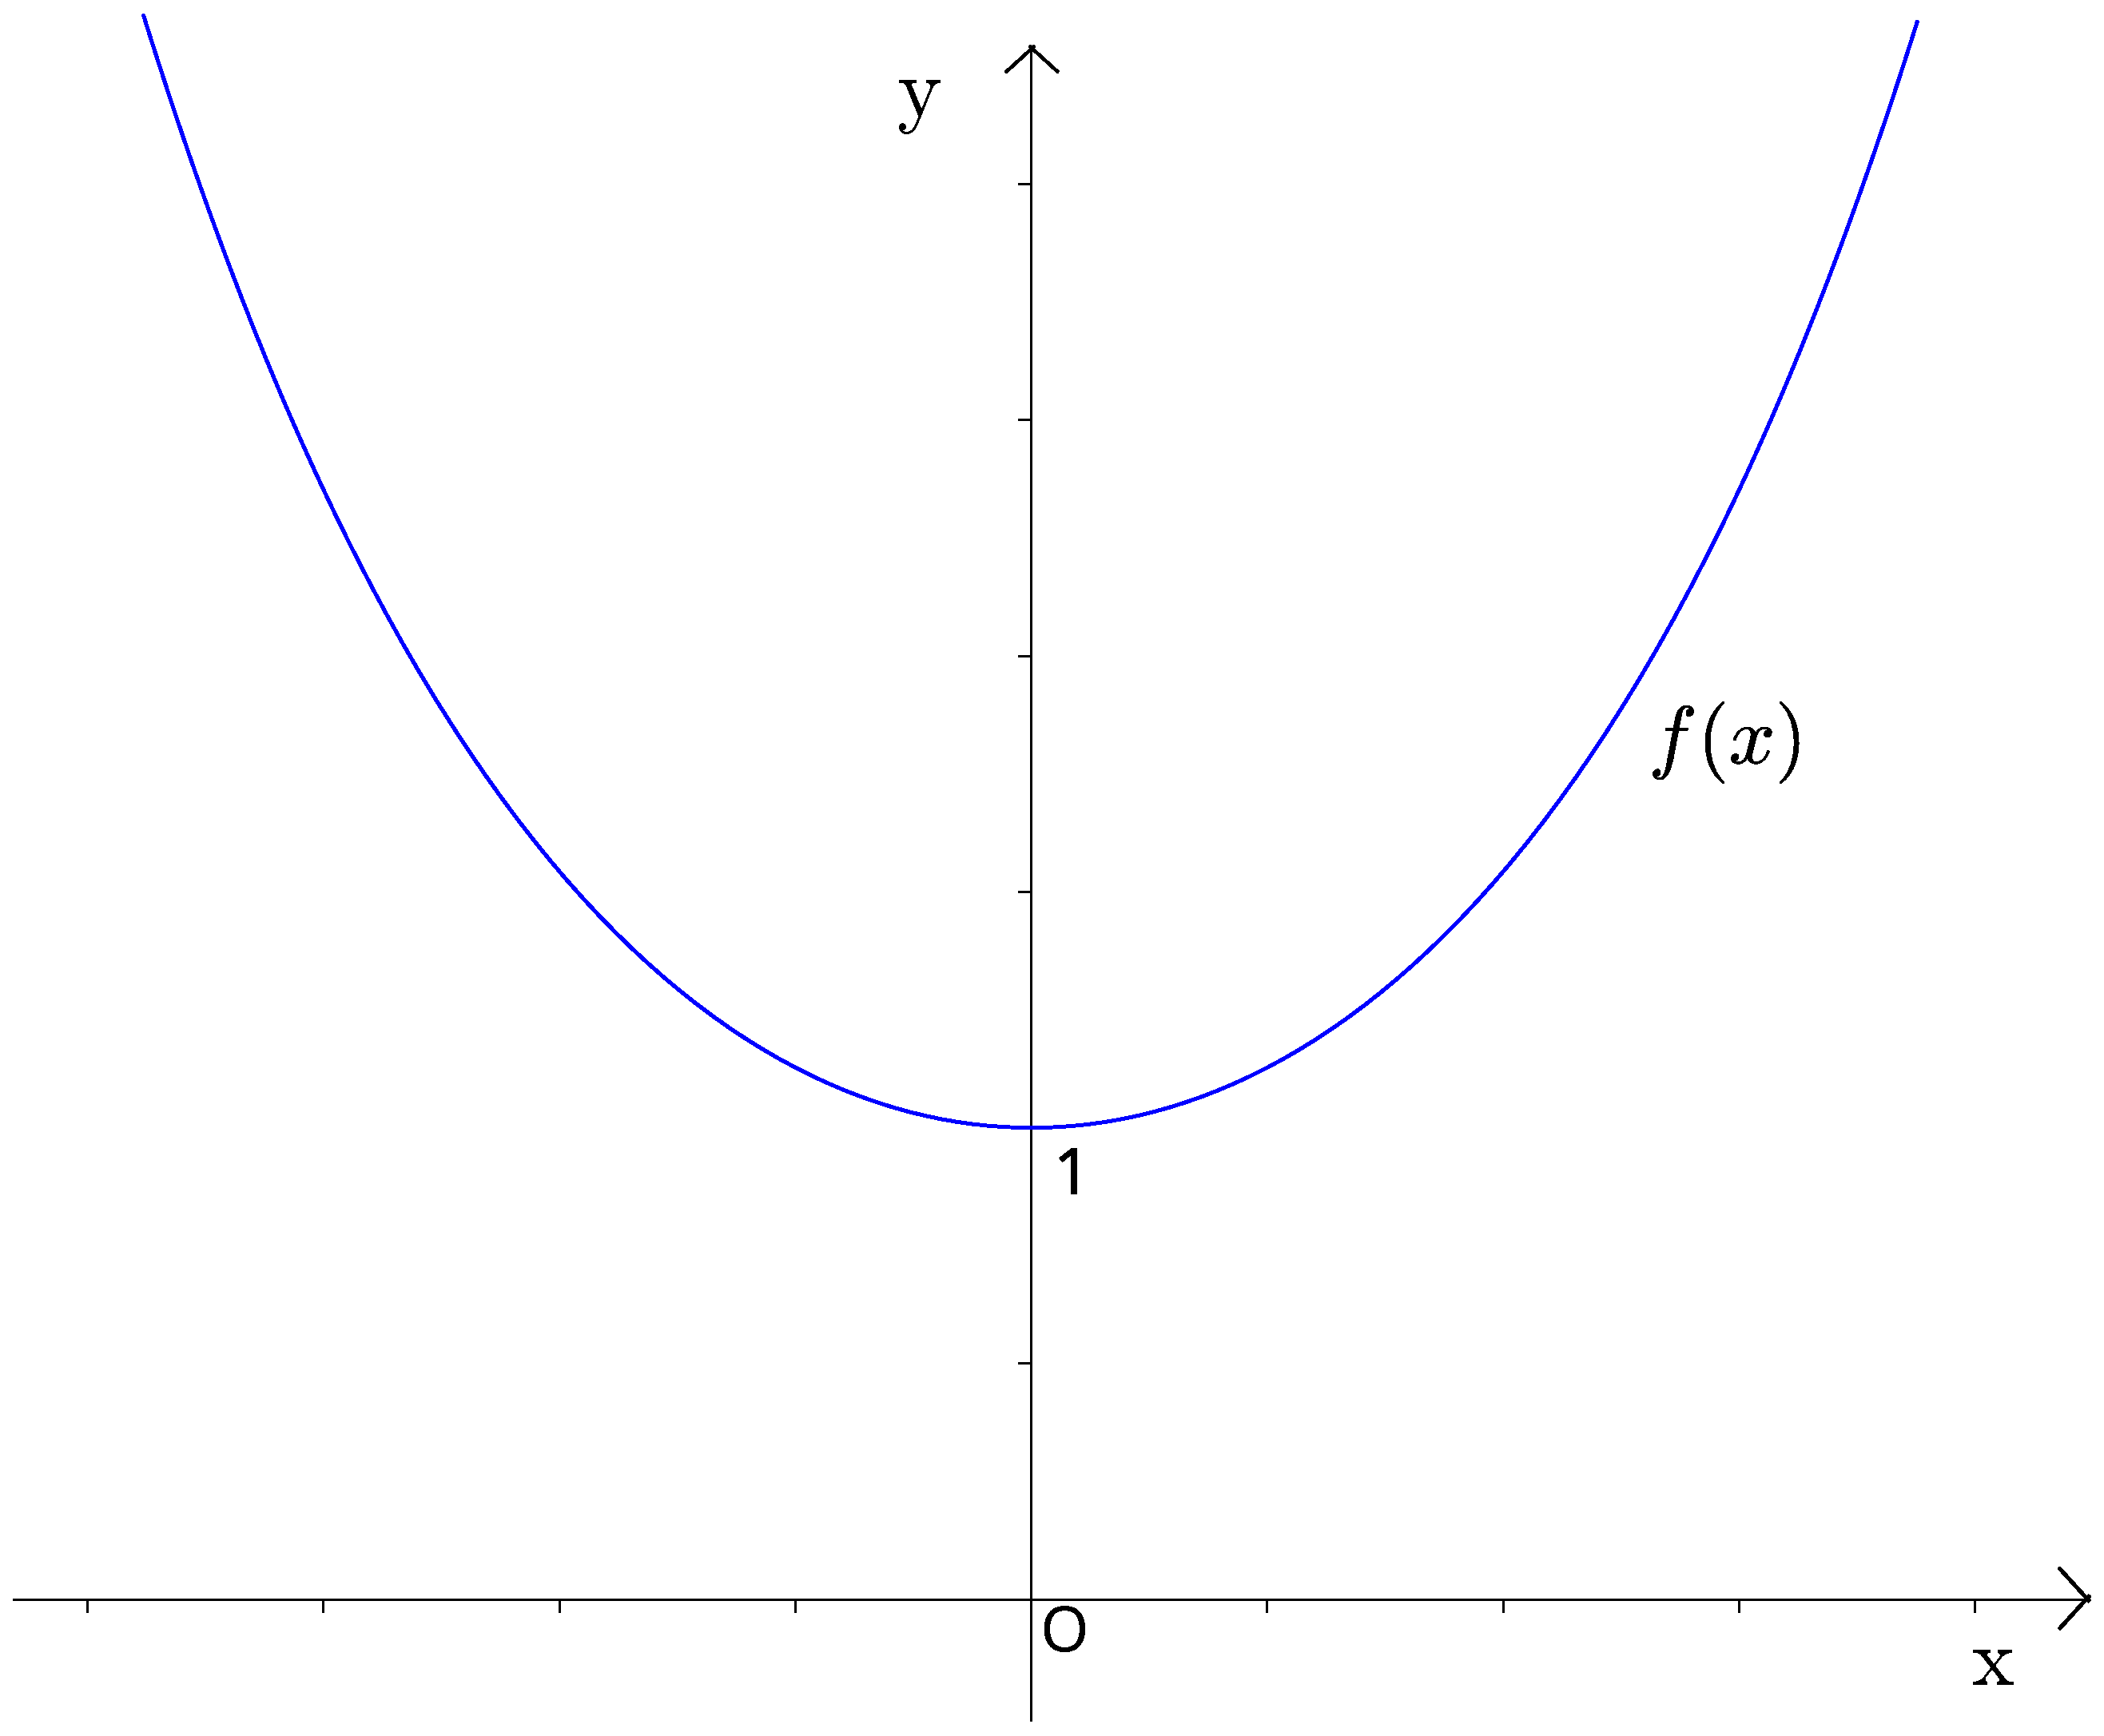
\includegraphics[width=\textwidth]{hyperbola-teorie2.eps}
					\caption{Funkce \textit{f}}
				\end{subfigure}%
				\begin{subfigure}{0.5\textwidth}
					\centering
					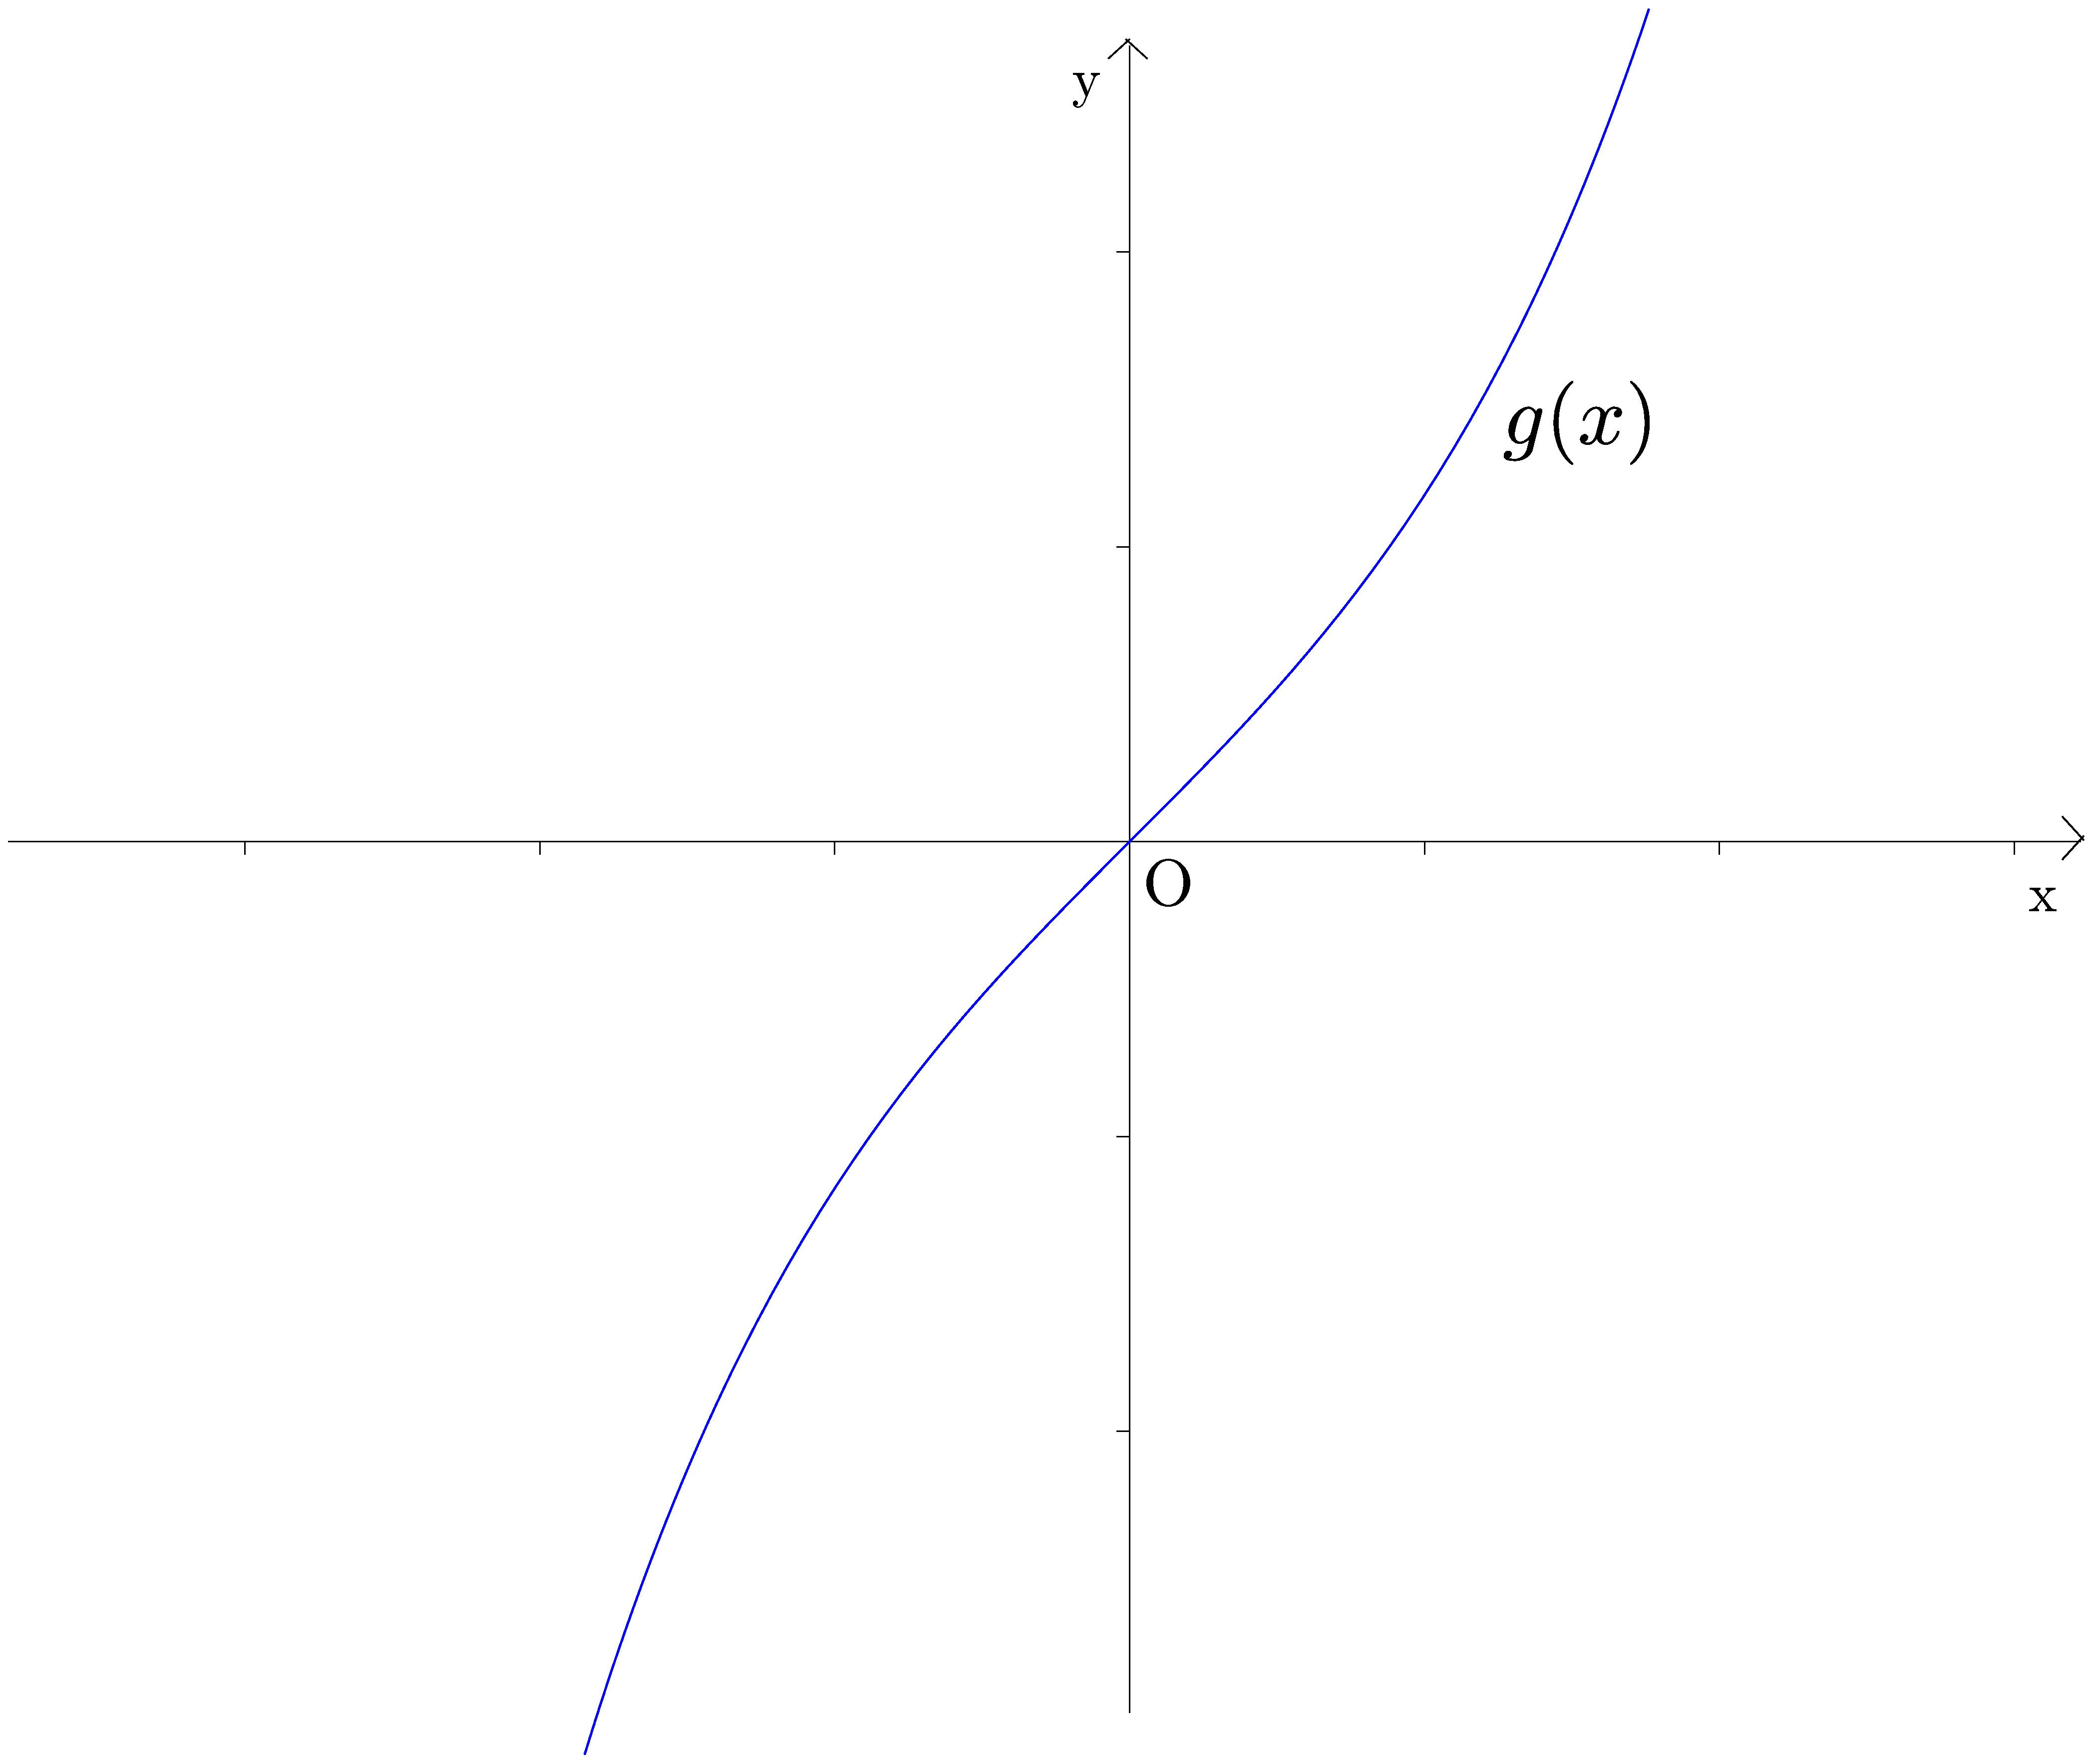
\includegraphics[width=\textwidth]{hyperbola-teorie3.eps}
					\caption{Funkce \textit{g}}
				\end{subfigure}
				\caption{Grafy hyperbolických funkcí \textit{f} a \textit{g}}
			\end{figure}
			\noindent Snadno ukážeme, že $f'(t)=g(t)$, $f''(t)=f(t)$, $g'(t)=f(t)$ a $f''(t)=g(t)$. \\[10pt]
			Něco podobného známe pro funkce  $\sin$ a $\cos$ (až na znaménka): $(cos{t})'=-\sin{t}$,\\ $(cos{t})''=-\cos{t}$
			, $(\sin{t})'=\cos{t}$ a $(sin{t})''=-\sin{t}$. \\[10pt]
			Proto se funkce $f(t)=\frac{e^t+e^{-t}}{2}$ nazývá  kosinus hyperbolický, značíme $\cosh{t}$. Funkce \\ $g(t)=\frac{e^t-e^{-t}}{2}$
			se nazývá sinus hyperbolický a značíme $\sinh{t}$. \\[10pt]
			Nyní si ověříme, že platí $\cosh^2{t}-\sinh^2{t}=1$:
			\begin{align*}
				\left(\frac{1}{2}(e^t+e^{-t})\right)^2                                             & - \left(\frac{1}{2}(e^t-e^{-t})\right)^2                                             \\
				\frac{1}{4} \left(e^{2t} + 2 e^t \cdot e^{-t} + e^{-2t}\right)                     & - \frac{1}{4} \left(e^{2t} - 2 e^t \cdot e^{-t} + e^{-2t}\right)                     \\
				\cancel{\frac{1}{4}e^{2t}}+\frac{1}{4} \cdot 2\cdot1 + \cancel{\frac{1}{4}e^{-2t}} & - \cancel{\frac{1}{4}e^{2t}}+\frac{1}{4} \cdot 2 \cdot 1-\cancel{\frac{1}{4}e^{-2t}} \\
				\frac{1}{2}+\frac{1}{2}                                                            & = 1                                                                                  
			\end{align*}
			\clearpage
			\noindent Pro parametrizaci hyperboly
			$$\frac{x^2}{a^2}-\frac{y^2}{b^2}=1$$
			dáme do rovnosti $\frac{x}{a}=\cosh{t}$ a $\frac{y}{b}=\sinh{t}$ a získáme parametrické vyjádření
			$$k(t)=\left[a\cosh{t}, b\sinh{t}\right], t \in \mathbb{R}.$$
			Toto je ovšem parametrický popis jedné větve hyperboly. \\
			Víme, že  $\cosh{t} \geq 1$ pro všechna $t \in \mathbb{R}$ (viz graf \textit{f}). Uvedený parametrický popis je popisem pravé větve hyperboly. Parametrický popis obou větví (symetrie podle osy \textit{y}) je
			$$k(t)=\left[\pm a\cosh{t}, b\sinh{t}\right], t \in \mathbb{R}.$$
			Pro parametrický popis hyperboly  $-\frac{x^2}{b^2}+\frac{y^2}{a^2}=1$ dáme do rovnosti $\frac{x}{b}=\sinh{t}$ a $\frac{y}{a}=\cosh{t}$ (zdůrazněme, že se rozhodujeme podle znamének v obecné rovnici). \\
			Parametrický popis obou větví je
			$$k(t)=\left[b\sinh{t}, \pm a\cosh{t} \right], t \in \mathbb{R}.$$
			(znaménko \textit{+} je pro horní větev, znaménko \textit{-} je pro dolní větev).
			Souřadnice vrcholů jsou $k(0)=[b\sinh{0}, \pm a\cosh{0}] = [0, \pm a \cdot 1] = [0, \pm a]$. \\
			Pro obecnější případ, kdy střed hyperboly je bod $S=[m, n]$ a rovnice ve středovém tvaru je
			$$\frac{(x-m)^2}{a^2}-\frac{(y-n)^2}{b^2}=1$$
			nebo
			$$-\frac{(x-m)^2}{b^2}+\frac{(y-n)^2}{a^2}=1$$
			změníme předchozí parametrizaci přičtením vektoru posunutí $S-O=(m, n)$. \\
			Parametrický popis hyperboly $\frac{(x-m)^2}{a^2}-\frac{(y-n)^2}{b^2}=1$ je
			$$k(t)=[m \pm a\cosh{t}, n+b\sinh{t}], t \in \mathbb{R}.$$
			parametrický popis hyperboly $-\frac{(x-m)^2}{b^2}+\frac{(y-n)^2}{a^2}=1$ je
			$$k(t)=[m+b\sinh{t}, n \pm a\cosh{t}], t \in \mathbb{R}.$$
			Při kreslení hyperboly s využitím grafického programu musíme interval pro parametr \textit{t} omezit z obou stran, např. $t \in \langle-10, 10 \rangle$
			\clearpage
			\subsection*{Příklad 1}
			Napište parametrické vyjádření hyperboly zadané obecnou rovnicí
			$$9x^2-16y^2-54x+128y-319=0.$$
			Napište souřadnice vrcholů a ohnisek hyperboly. Dále napište obecné rovnice asymptot. \\[10pt]
			\textbf{Řešení:} Obecnou rovnici upravíme na středový tvar:
			$$\frac{(x-3)^2}{16}-\frac{(y-4)^2}{9}=1.$$
			Střed hyperboly je bod $S=[3,4]$, hlavní osa je rovnoběžná s osou \textit{x}. Velikost hlavní poloosy
			je $a=4$, velikost vedlejší poloosy je $b=3$. \\
			Pro parametrizaci dáme do rovnosti \\
			\begin{align*}
				\frac{x-3}{4} & =\cosh{t}, \\ \frac{y-4}{3}&=\sinh{t}
			\end{align*}
			a získáme parametrický popis pravé větve
			$$k(t)=[3+4\cosh{t}, 4+3\sinh{t}], t \in \mathbb{R}\text{.}$$
			Parametrický popis obou větví je
			$$k(t)=[3\pm4\cosh{t}, 4+3\sinh{t}], t \in \mathbb{R}\text{.}$$
			Vrcholy můžeme vypočítat z parametrického vyjádření
			\begin{align*}
				k(0)=[3\pm4\cdot1, 4+3\cdot0] \text{,} \\
				\text{tedy }                           
				A=[7, 4], B=[-1, 4].                   
			\end{align*}
			Pro velikost excentricity \textit{e} platí vztah $e^2=a^2+b^2$. V našem případě \\ $e^2=16+9$
			a tedy $e=5$.
			\begin{align*}
				E & =[3+5, 4]=[8, 4] \\
				F & =[3-5, 4]=[-2,4] 
			\end{align*}
			Rovnice asymptot získáme z rovnice
			\begin{align*}
				\frac{(x-3)^2}{16}    & -\frac{(y-4)^2}{9}=0      \\
				\text{tj.: } 9(x-3)^2 & -16(y-4)^2=0              \\
				[3(x-3)]^2            & -[4(y-4)]^2=0             \\
				[3(x-3)-4(y-4)]       & \cdot[3(x-3)+4(y-4)] = 0. 
			\end{align*}
			Rovnice asymptot jsou
			\begin{align*}
				a_1: 3x-4y+7  & =0  \\
				\text{a}\\
				a_2: 3x+4y-25 & =0. 
			\end{align*}
			\begin{figure}[H]
				\centering
				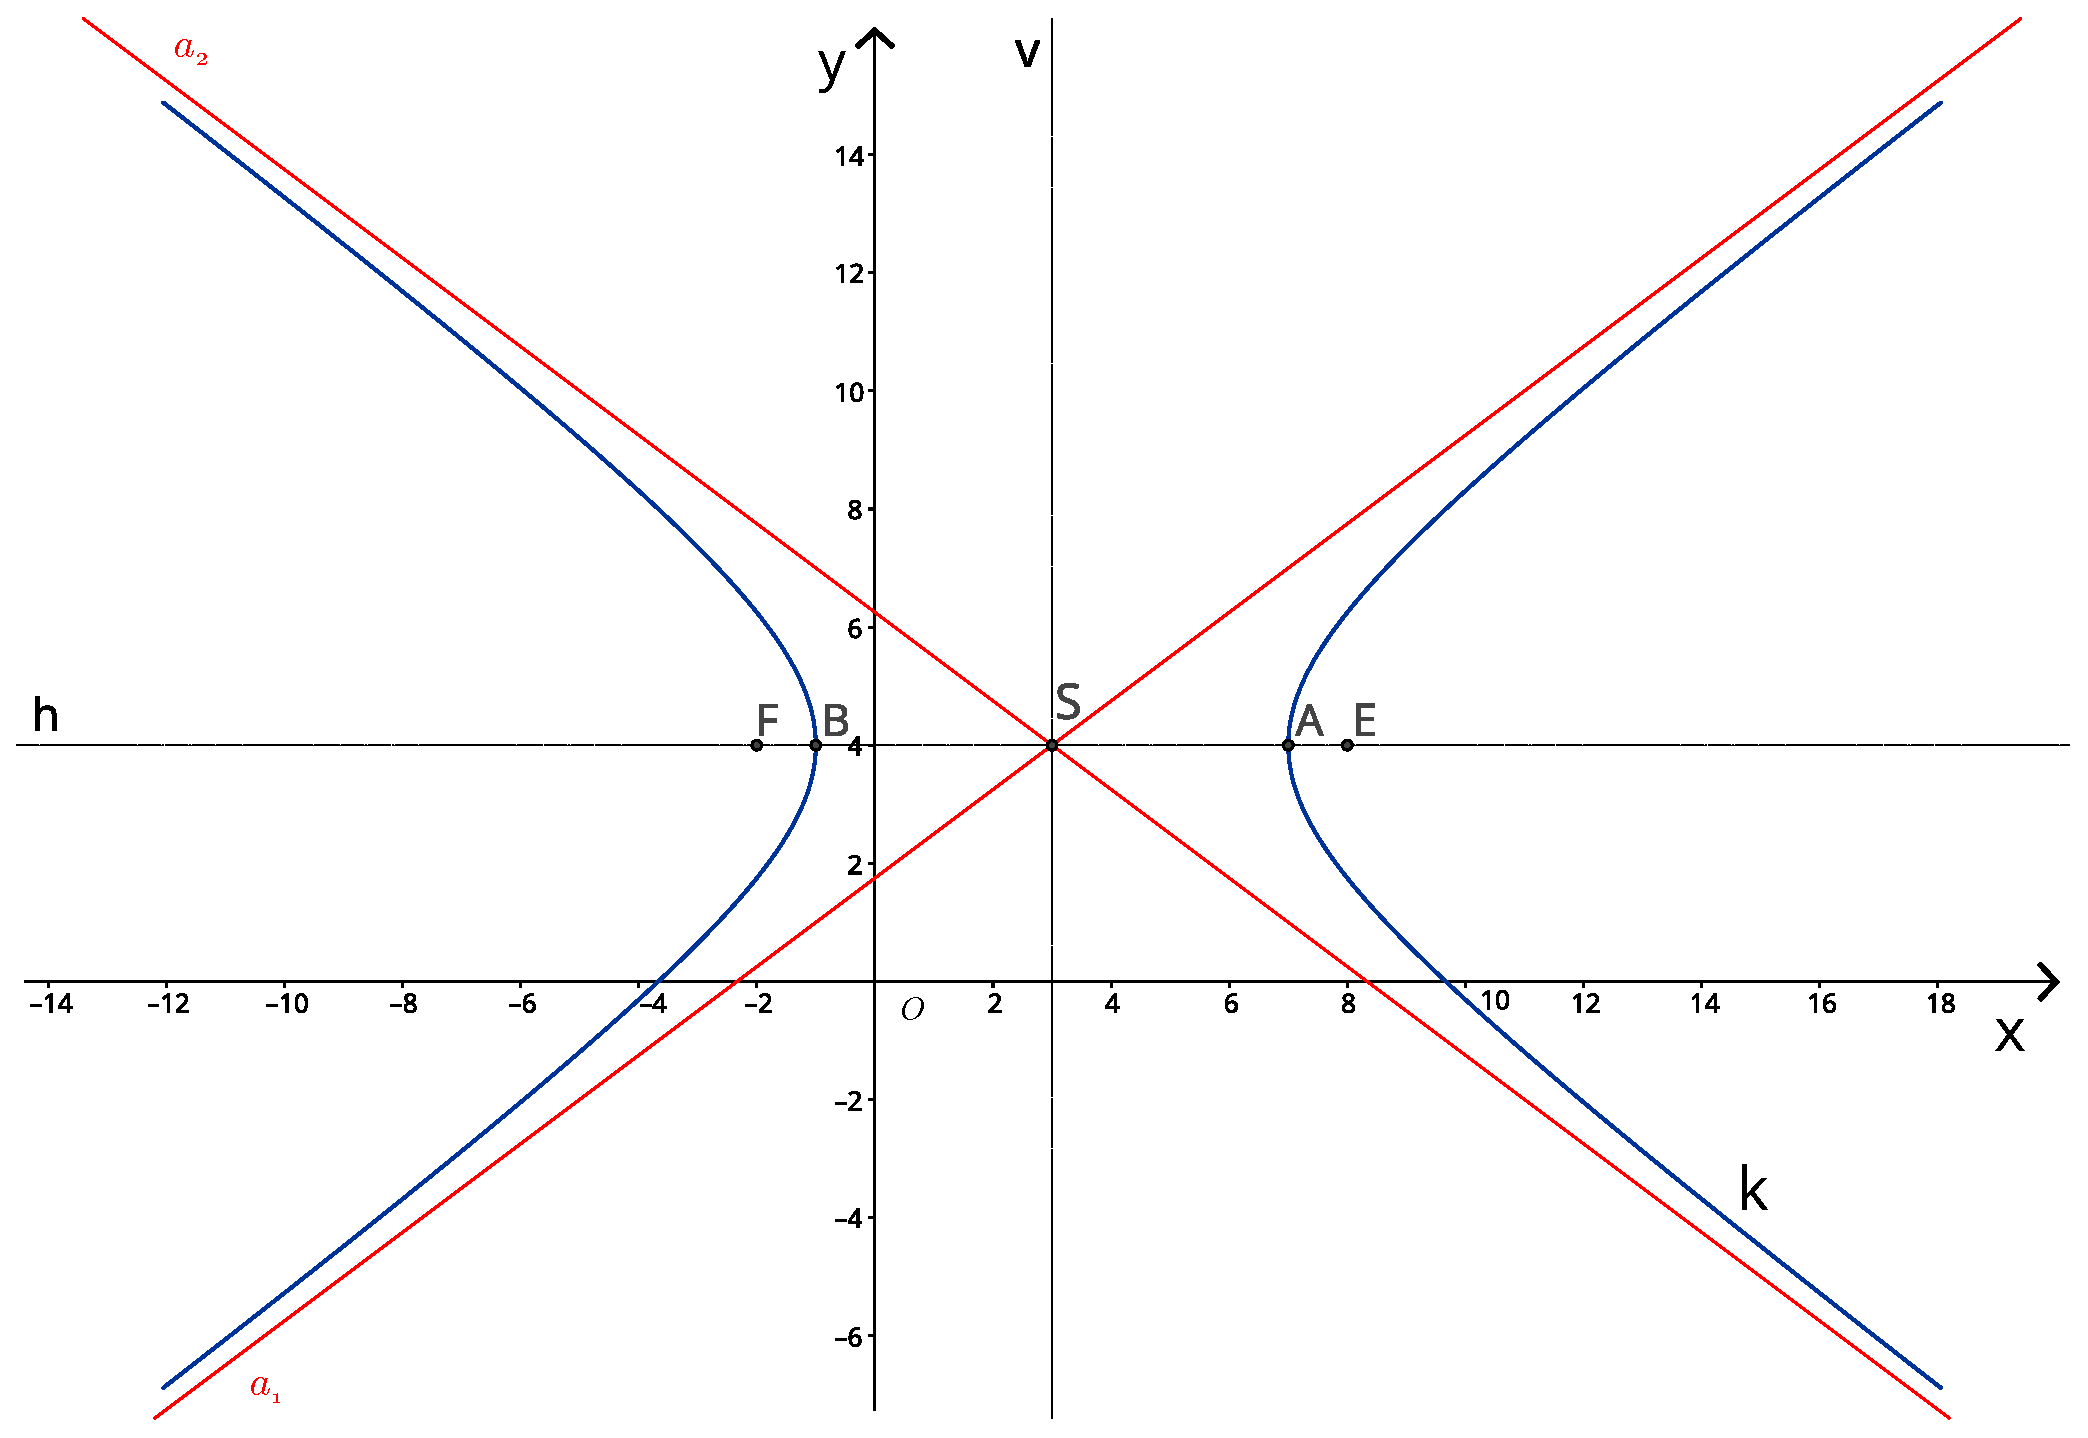
\includegraphics[width=\textwidth]{hyperbola1.eps}
				\caption{Hyperbola pro $t \in \langle-2, 2\rangle$}
									
			\end{figure}
			\clearpage
			\subsection*{Příklad 2}
			Napište parametrické vyjádření hyperboly zadané obecnou rovnicí
			$$9x^2-16y^2-54x+128y-31=0.$$
			Napište souřadnice vrcholů, ohnisek a průsečíků hyperboly se souřadnicovými osami. Dále napište obecné rovnice asymptot.\\[5pt]
			\textbf{Řešení:} Obdobně jako v minulém příkladu upravíme obecnou rovnici na středový tvar:
			$$\frac{(y-4)^2}{9}-\frac{(x-3)^2}{16}=1.$$
			Střed hyperboly je bod $S=[3,4]$, hlavní osa je rovnoběžná s osou \textit{y}. Velikosti poloos jsou $a=3$ a $b=4$. \\
			Pro parametrizaci dáme do rovnosti \\
			\begin{align*}
				\frac{y-4}{3} & =\cosh{t}, \\ \frac{x-3}{4}&=\sinh{t}
			\end{align*}
			a získáme parametrický popis horní větve
			$$k(t)=[3+4\sinh{t}, 4+3\cosh{t}], t \in \mathbb{R}\text{.}$$
			Parametrický popis obou větví je
			$$k(t)=[3+4\sinh{t}, 4\pm3\cosh{t}], t \in \mathbb{R}\text{.}$$
			Vrcholy můžeme vypočítat z parametrického vyjádření
			\begin{align*}
				k(0)=[3+4\cdot0, 4\pm3\cdot1] \text{,} \\
				\text{tedy }                           
				A=[3, 7], B=[3, 1].                    
			\end{align*}
			Pro velikost excentricity \textit{e} platí vztah $e^2=a^2+b^2$. V našem případě \\ $e^2=9+16$
			a tedy $e=5$.
			\begin{align*}
				E & =[3, 4+5]=[3, 9] \\
				F & =[3, 4-5]=[3,-1] 
			\end{align*}
			Rovnice asymptot získáme z rovnice
			\begin{align*}
				\frac{(y-4)^2}{9}-\frac{(x-3)^2}{16}=0 \\
				\text{tj.: } 16(y-4)^2-9(x-3)^2 & =0                        \\
				[4(y-4)]^2-[3(x-3)]^2           & =0                        \\
				[4(y-4)-3(x-3)]                 & \cdot[4(y-4)+3(x-3)] = 0. 
			\end{align*}
			Rovnice asymptot jsou
			\begin{align*}
				a_1 & : 3x-4y+7  =0  \\
				\text{a}\\
				a_2 & : 3x+4y-25 =0. 
			\end{align*}
			Souřadnice průsečíků hyperboly se souřadnicovými osami můžeme určit a) z obecné rovnice nebo b) z rovnice ve středovém tvaru
			nebo c) z parametrického vyjádření.
			\begin{enumerate}
				\item Průsečíky s osou \textit{x} ($y=0$) \\
				      \small
				      \begin{minipage}[t]{0.5\textwidth}
				      	a)
				      	\begin{align*}
				      		9x^2    & -54x-31=0                     \\
				      		x_{1,2} & = \frac{54\pm\sqrt{4032}}{18} \\
				      		x_{1,2} & = \frac{54\pm24\sqrt{7}}{18}  \\
				      		x_1     & = 3 + \frac{4\sqrt{7}}{3}     \\
				      		x_2     & = 3 - \frac{4\sqrt{7}}{3}     
				      	\end{align*}
				      \end{minipage}
				      \begin{minipage}[t]{0.5\textwidth}
				      	b)
				      	\begin{align*}
				      		\frac{16}{9}-\frac{(x-3)^2}{16} & = 1                       \\
				      		-\frac{(x-3)^2}{16}             & = -\frac{7}{9}            \\
				      		(x-3)^2                         & = \frac{7}{9}\cdot16      \\
				      		|x-3|                           & = \frac{4\sqrt{7}}{3}     \\
				      		x_1                             & = 3 + \frac{4\sqrt{7}}{3} \\
				      		x_2                             & = 3 - \frac{4\sqrt{7}}{3} 
				      	\end{align*}
				      \end{minipage}
				      c) průsečíky s osou \textit{x} má pouze dolní větev
				      				      
				      \begin{minipage}[t]{0.5\textwidth}
				      	\begin{align*}
				      		4-3\cosh{t}=0                       \\
				      		4-3\cdot\frac{1}{2}(e^t+e^{-t}) = 0 \\
				      		8-3\cdot(e^t+e^{-t}) = 0            \\
				      		8-3e^t-3\frac{1}{e^t} = 0           \\
				      		8e^t-3(e^t)^2-3 = 0                 \\
				      		3(e^t)^2-8e^t+3 = 0                 \\
				      		e^t = \frac{8\pm\sqrt{28}}{6}       \\
				      		e^t = \frac{4\pm\sqrt{7}}{3}        
				      	\end{align*}
				      \end{minipage}				    
				      \begin{minipage}[t]{0.5\textwidth}
				      	\vspace{10pt}
				      	pro $e^t=\frac{4+\sqrt{7}}{3}$ je $\sinh{t} = \frac{1}{2}(e^t-\frac{1}{e^t})=$
				      	\begin{align*}
				      		  & = \frac{1}{2}(\frac{4+\sqrt{7}}{3}-\frac{3}{4+\sqrt{7}}) =    \\
				      		  & = \frac{1}{2}(\frac{4+\sqrt{7}}{3}-\frac{3(4-\sqrt{7})}{9}) = \\
				      		  & = \frac{1}{2}\cdot\frac{2\sqrt{7}}{3} = \frac{\sqrt{7}}{3}    
				      	\end{align*}
				      	pro $e^t=\frac{4-\sqrt{7}}{3}$ je $\sinh{t} = \frac{1}{2}(\frac{4-\sqrt{7}}{3}-\frac{3}{4-\sqrt{7}}) = -\frac{\sqrt{7}}{3}$
				      	\begin{align*}
				      		x_1 & = 3 + \frac{4\sqrt{7}}{3} \\
				      		x_2 & = 3 - \frac{4\sqrt{7}}{3} 
				      	\end{align*}
				      \end{minipage}
				      \vspace{10pt}
				      Z výpočtu je vidět, že nejrychlejší výpočet vychází z rovnice ve středovém tvaru. Průsečíky s osou \textit{x} jsou body
				      $P_1=\left[3 + \frac{4\sqrt{7}}{3}, 0\right]$ a $P_2=\left[3-\frac{4\sqrt{7}}{3}, 0\right]$.
				      \normalsize
				\item Průsečíky s osou \textit{y} ($x=0$) vypočítáme z rovnice ve středovém tvaru:
				      \begin{align*}
				      	\frac{(y-4)^2}{9}-\frac{9}{16} & = 1                               \\
				      	\frac{(y-4)^2}{9}              & = 1+\frac{9}{16}                  \\
				      	(y-4)^2                        & = \frac{25}{16}\cdot 9            \\
				      	|y-4|                          & = \frac{5\cdot3}{4}               \\
				      	y_1                            & = 4 + \frac{15}{4} = \frac{31}{4} \\
				      	y_2                            & = 4 - \frac{15}{4} = \frac{1}{4}  
				      \end{align*}
				      Průsečíky s osou \textit{y} jsou body $P_4=\left[0, \frac{31}{4}\right]$ a $P_3=\left[0, \frac{1}{4}\right]$.
			\end{enumerate}
			\vfill
			\begin{figure}[H]
				\centering
				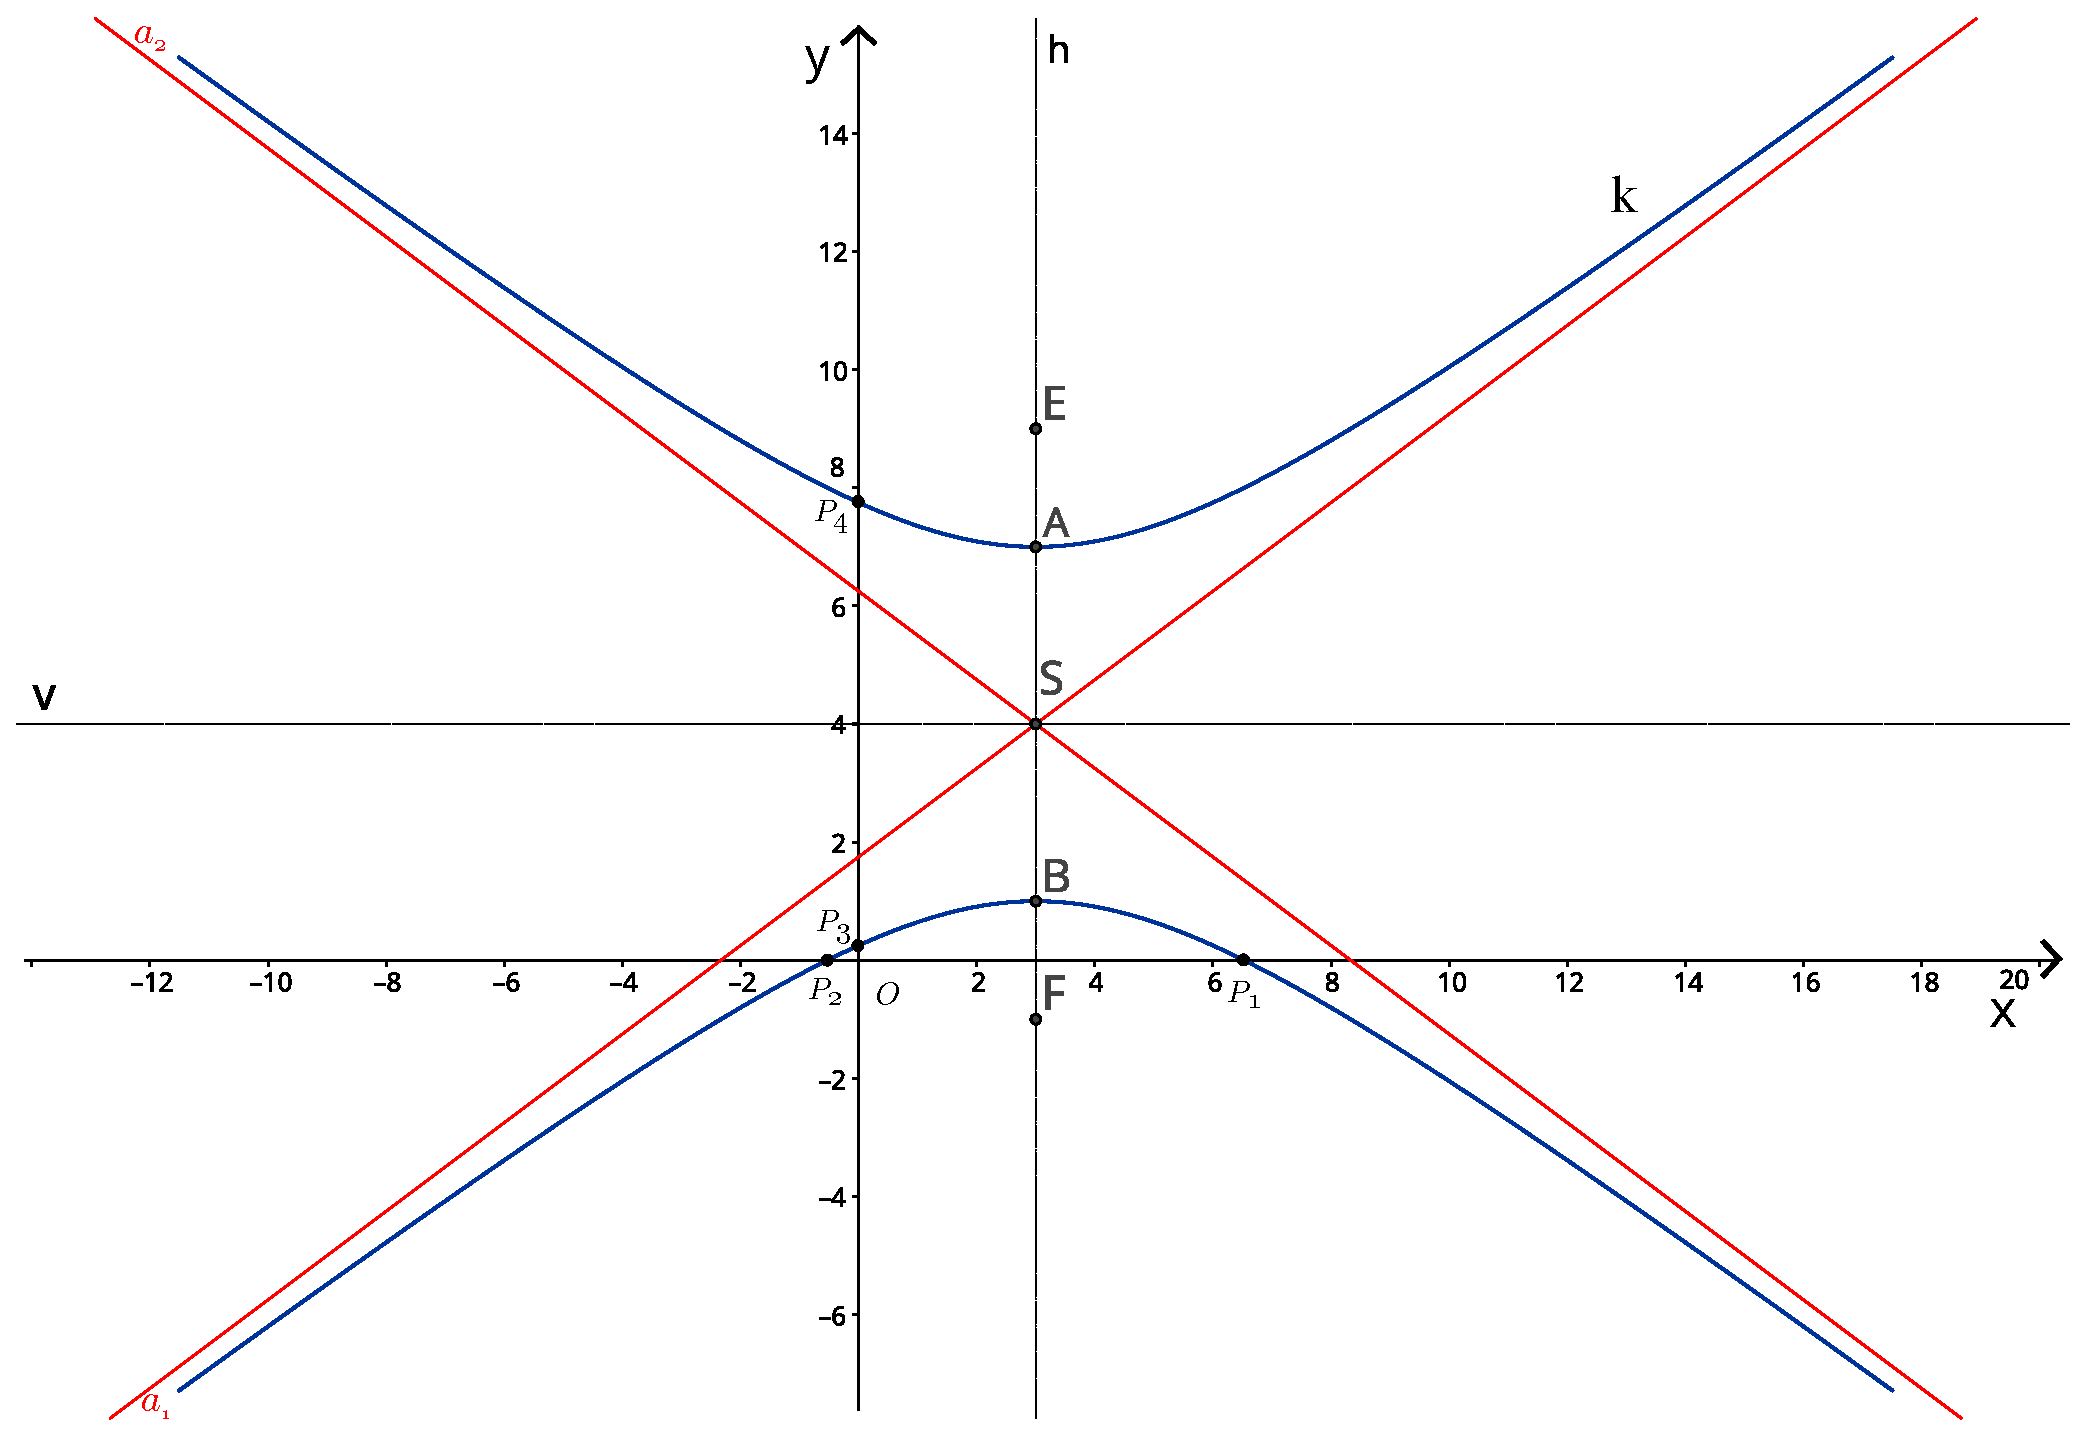
\includegraphics[width=\textwidth]{hyperbola2.eps}
				\caption{Hyperbola pro $t \in \langle-2, 2\rangle$}
									
			\end{figure}